%%%*******************************************************************************
%  Classe Latex tprax, Version 0.0.0 31/10/2017
%
%  Define as normas e estilo das dissertações, teses ou tcc do SENAI CIMATEC
%
%%%-------------------------------------------------------------------------------

%%%-------------------------------------------------------------------------------
% Changes log
%%%-------------------------------------------------------------------------------
% Version 0.0.0 - 00/00/2000
% - 
%%%-------------------------------------------------------------------------------

%%%-------------------------------------------------------------------------------
%  DOCUMENTATION WITH EXAMPLE
%%%*******************************************************************************

%%%-------------------------------------------------------------------------------
%%% Thesis default options
%%%-------------------------------------------------------------------------------
%\documentclass[subook]{Classes/tprax}
%\documentclass[sureport]{Classes/tprax}

%%%-------------------------------------------------------------------------------
%%% Thesis custom options
%%%-------------------------------------------------------------------------------

%%% Fancy page headings
%\documentclass[fancyheadings, subook]{Classes/tprax}
%\documentclass[fancyheadings, sureport]{Classes/tprax}

%%% Fancy chapters and sections headings
%\documentclass[fancychapter, subook]{Classes/tprax}
%\documentclass[fancychapter, sureport]{Classes/tprax}

%%% Fancy page , chapters and sections headings
%\documentclass[fancyheadings, fancychapter, subook]{Classes/tprax}
%\documentclass[fancyheadings, fancychapter, sureport]{Classes/tprax}
\documentclass[fancyheadings, fancychapter, sureport]{Classes/tprax}

%%%-------------------------------------------------------------------------------
%%% Thesis Commands (ONLY with fancy page headings)
%%%-------------------------------------------------------------------------------

%%%Page header line width
%\footlinewidth{value}

%%%Page footer line width
%\headlinewidth{value}

%%%Page header and footer line width
%\headingslinewidth{value}

%%%Page header and footer lines without text
%\headingslinesonly

%%%The default line width is 0.3pt.
%%%Set the value to 0pt to remove the page header and/or footer line

%%%-------------------------------------------------------------------------------
%%% SUThesis Supported Graphic Formats
%%%-------------------------------------------------------------------------------
% The figures formats supported depend upon the selected output file
% Include your figure without the extention, the SUThesis will automatically
% search the predefined `Figures' directory tree for the right file format.
%
% - The pdfLaTEX (PDF) supports graphics inclusions in PDF, JPG, PNG, and
%   MetaPost (with .mps extention) formats.
%
% - The Latex (DVI) supports graphics inclusions in EPS and PS formats.
%%%-------------------------------------------------------------------------------


%%%-------------------------------------------------------------------------------
%%% Árvore de diretório tprax
%%%-------------------------------------------------------------------------------
%  Diretório
%       \Classes        (requerido)
%       \Figures        (requerido) --------------------------------->
%       \Figures\PDF    (optional)
%       \Figures\JPG    (optional) Figures located within these
%       \Figures\PNG    (optional) folders are searched automatically
%       \Figures\MPS    (optional)  by the tprax class.
%       \Figures\EPS    (optional)
%       \Figures\PS     (optional) <--------------------------------
%       \Tables         (requerido)
%       \Others         (requerido)
%       \Chapters       (requerido)
%       \Appendices     (optional)
%       \References     (requerido)
%%%-------------------------------------------------------------------------------

%%%-------------------------------------------------------------------------------
%%% PDF File Summary
%%%-------------------------------------------------------------------------------
\ifpdf
    \hypersetup{backref,
                colorlinks  = true,
                pdftitle    = Modelo de visualização de informação de redes complexas utilizando sistemas de identificação de gestos e realidade virtual,
                pdfauthor   = {Marco Reis, marco.a.reis@gmail.com},
                pdfsubject  = Mestre em Engenharia,
                pdfcreator  = Subtitulo,
                pdfproducer = PDFLatex,
                pdfkeywords = {Palavra-chave1, Palavra-chave2, Palavra-chave3}
    }
 \fi

%%%-------------------------------------------------------------------------------
%%% Required packages
%%%-------------------------------------------------------------------------------
% - ifthen
% - setspace
% - amsmath
% - amsfonts
% - amssymb
% - amsthm
% - eucal
% - graphics
% - fancyhdr
%%%-------------------------------------------------------------------------------

%%%-------------------------------------------------------------------------------
%%% Optional packages
%%%-------------------------------------------------------------------------------
%\usepackage[latin1]{inputenc}
\usepackage[utf8]{inputenc}
\usepackage[brazil]{babel}
\usepackage{longtable}
\usepackage{dcolumn}
\usepackage{multirow}
\usepackage{lscape}
\usepackage{graphicx}
\usepackage{rotating}
\usepackage{float,subfigure}
\usepackage{cite}
\usepackage[left=3cm,top=3cm,right=2cm,bottom=2cm]{geometry}
%\usepackage[alf,abnt-etal-list=5]{abntcite}
\usepackage[alf]{abntex2cite}
\usepackage{ifpdf}
\usepackage{shadow}
\usepackage{wrapfig}
\usepackage[normalem]{ulem}
\usepackage{makeidx} % cria indice remissivo
\usepackage{yfonts}
\makeindex % cria o indice remissivo
%Tables and Figures Caption
\setlength{\LTcapwidth}{\textwidth}





%\usepackage{algorithm}
%\usepackage{algorithmic}




%\newtheorem{theorem}{Teorema}
%\newtheorem{definition}[theorem]{Defini\c{c}\~ao}


%%%-------------------------------------------------------------------------------
%%% Start thesis root document
%%%-------------------------------------------------------------------------------
\begin{document}
    %%----------------------------------------------------------------------------
    %% Define the title page
    %%----------------------------------------------------------------------------
    \university{Centro Universitário SENAI CIMATEC}
%    \faculty{Pro\-gra\-ma de P\'os-gra\-dua\-\c{c}\~ao em Mo\-de\-la\-gem Com\-pu\-ta\-cio\-nal e Tec\-no\-lo\-gia In\-dus\-trial}
    %\faculty{Centro Universitário Senai Cimatec}
%    \school{School of Mathematics}
% ********************************************** TCC ****************
    \course{Engenharia de Automação e Controle}
    \coursee{Engenharia Mecânica}
    \typework{Projeto Theoprax de Conclusão de Curso}
% ********************************************************************
% ********************************************* Mestrado ******************
%    \course{Mestrado em Modelagem Computacional e Tecnologia Industrial}
%    \typework{Disserta\c{c}\~ao de mestrado}
%    \typework{Exame de Qualificação de Mestrado}
% ********************************************** Doutorado ****************
%    \course{Engenharia Elétrica}
%    \typework{Tese de doutorado}
%    \typework{Exame de Qualificação de doutorado}
% ********************************************************************
 \thesistitle{Doogie: um projeto de robô micromouse}
    \hidevolume
    \thesisvolume{Volume 1 of 1}
    \thesisauthor{Caio Amaral}
    \thesisauthorr{Élisson Riller}
    \thesisauthorrr{Elton Marques}
    \thesisauthorrrr{Iure Pinheiro}
    \thesisauthorrrrr{Mateus Menezes}
    \thesisadvisor{Prof. Marco Reis, M.Eng.}
    \hidecoadvisor
    %\thesiscoadvisor{Marco Reis}
    \thesisdegreetitle{Bacharel em Engenharia}
    %\thesisdegreetitle{Doutor em }
%    \thesismonthyear{M\^es de Ano}
    \thesismonthyear{Setembro de 2019}


    \maketitlepage

    %%----------------------------------------------------------------------------
    %% Inserir Folha de rosto, Nota de estilo, folha de assinaturas, dedicatoria
    %%----------------------------------------------------------------------------
    \begin{folharosto}

\begin{center}
\theauthor \\
\theauthorr \\
\theauthorrr \\
\theauthorrrr \\
\theauthorrrrr \\

\end{center}
\ \\
\ \\
\ \\
\ \\
\ \\
\begin{spacing}{2}
   \begin{center}
   {\LARGE {\bf \thetitle}}
   \end{center}
\end{spacing}
\ \\
\ \\
\ \\
\begin{flushright}

   \begin{list}{}{
      \setlength{\leftmargin}{7.5cm}
      \setlength{\rightmargin}{0cm}
      \setlength{\labelwidth}{0pt}
      \setlength{\labelsep}{\leftmargin}}

      \item \thetypework apresentada ao \thefaculty, Curso de \thecourse e \thecoursee
      do \theuniversity, como requisito parcial para a obten\c{c}\~ao do
      t\'itulo de {\bf \thedegreetitle}.

      \begin{list}{}{
      \setlength{\leftmargin}{0cm}
      \setlength{\rightmargin}{0cm}
      \setlength{\labelwidth}{0pt}
      \setlength{\labelsep}{\leftmargin}}

      \item \'Area de conhecimento: Interdisciplinar

      \item Orientador: \theadvisor
      \newline \hspace*{2.1cm}  %{\it \theuniversity}

      \end{list}
   \end{list}

\end{flushright}
\ \\
\ \\
\ \\
\ \\
%\begin{spacing}{1.5}
   \begin{center}
   Salvador \par
   \theuniversity \par
   2019
   \end{center}
%\end{spacing}

\end{folharosto}

    %\begin{notaestilo}
Esta \thetypeworkthree foi elaborada considerando as normas de
estilo (i.e. est\'eticas e estruturais) propostas aprovadas pelo
colegiado do \thefacultytwo e est\~ao dispon\'iveis em formato
eletr\^onico ({\it download} na P\'agina Web
http:$//$ead.fieb.org.br$/$portal\_faculdades$/$dissertacoes-e-teses-mcti.html
ou solicita\c{c}\~ao via e-mail \`a secretaria do
programa) e em formato impresso somente para consulta. \\

Ressalta-se que o formato proposto considera diversos itens das
normas da Associa\c{c}\~ao Brasileira de Normas T\'ecnicas (ABNT),
entretanto opta-se, em alguns aspectos, seguir um estilo pr\'oprio
elaborado e amadurecido pelos professores do programa de
p\'os-gradua\c{c}\~ao supracitado.

\end{notaestilo}

    %\begin{folhaassinaturas}

%\thispagestyle{empty}

\def\signature#1#2{\parbox[b]{1in}{\smash{#1}\vskip12pt}
\hfill \parbox[t]{3in}{\shortstack{\vrule width 3in height
0.4pt\\\small#2}}}

\def\InstituicaoMembro#1#2{\parbox[b]{1in}{\smash{#1}\vskip12pt}
\hfill \parbox[t]{3in}{\shortstack{\vrule width 3in \\\small#2}}}

\def\signaturepage{%

    \begin{spacing}{1.5}
        \begin{center}
        {\LARGE \theuniversity} \\
        {\large \thefaculty} \\
        {\large \thecourse} \\
        \end{center}
    \end{spacing}

   \vskip 0.25in plus 0.4in minus 0.1in

    \begin{spacing}{1.5}
        \begin{sloppypar}
        A Banca Examinadora, constitu\'ida pelos professores abaixo
        listados, leram e recomendam a aprova\c{c}\~ao [com distin\c{c}\~ao] da
        \thetypeworktwo, intitulada ``\thetitle",
        apresentada no dia (dia) de (m\^es) de (ano), como requisito
        parcial para a obten\c{c}\~ao do t\'itulo de {\bf \thedegreetitle}.\\
        \end{sloppypar}
    \end{spacing}

    \def\sigskip{\vskip0.15in plus 0.2in minus 0.1in}
    \def\beginskip{\vskip0.3875in plus 0.2in minus 0.1in}

    \beginskip
    \signature{Orientador:}{Prof. Dr. \theadvisor} \\
    \InstituicaoMembro{}{\theuniversity} \\

    \sigskip
    \beginskip
    \signature{Membro externo da Banca:}{Prof. Dr. Nome completo} \\
    \InstituicaoMembro{}{Institui\c{c}\~ao do membro da banca} \\

    \sigskip
    \beginskip
    \signature{Membro externo da Banca:}{Prof. Dr. Nome completo} \\
    \InstituicaoMembro{}{Institui\c{c}\~ao do membro da banca} \\

    %\sigskip
    %\beginskip
   % \signature{Membro interno da Banca:}{Prof. Dr. Nome completo} \\
   % \InstituicaoMembro{}{Institui��o do membro da banca} \\

    \vfill
    \newpage
    \setcounter{page}{3}
}
%*********************************************************************


\signaturepage


\end{folhaassinaturas}

    \include{Others/dedicatoria}
    \begin{agradecimentos}
	content...
\end{agradecimentos}


    %%----------------------------------------------------------------------------
    %% Resumo/abstract, sumário e siglas
    %%----------------------------------------------------------------------------
    \begin{romanpagenumbers}
        \begin{thesisresumo}
Escreva aqui o resumo da disserta\c{c}\~ao, incluindo os contextos geral e espec\'ifico, dentro dos quais a pesquisa foi realizada, o objetivo da pesquisa, assun\c{c}\~ao filos\'ofica, os m\'etodos de pesquisa usados e as poss\'iveis contribui\c{c}\~oes que o que \'e proposto pode trazer \`a sociedade.

\ \\

% use de três a cinco palavras-chave

\textbf{Palavras-chave}: Palavra-chave 1, Palavra-chave 2, Palavra-chave 3, Palavra-chave 4, Palavra-chave 5

\end{thesisresumo}

        \begin{thesisabastract}
Studies in Artificial Intelligence have grown and diversified in different applications, and often associated with robotics, increasingly requiring trained professionals for its use and exploration in different environments. Because of this need, open robotics platforms can be a potential solution for introductory learning in these two areas. Therefore, the objective of this work is to develop an open source platform based on the models used in the Micromouse competition. This platform will consist of a prototype, a simulation environment and a test maze. A methodology divided into four parts was used: conceptual, design, development and conclusion. The phases of this methodology generated materials that culminated in the elaboration of two prototypes with assembly and configuration guides, a simulation environment using ROS and Gazebo, a modular maze proposal and a robot control software package. Finally, it is presented at the end of the work the conclusions obtained, possible approaches to use the platform and future work.

\ \\


\textbf{Keywords}: Artificial Intelligence, Mobile Robotics, Robotics Teaching

\end{thesisabastract}

        % Make list of contents, tables and figures
        \thesiscontents
        %Include other required section
        \newacronym{ros}{ROS}{\textit{Robot Operating System}}
\newacronym{ia}{IA}{Inteligência Artificial}
\newacronym{ibm}{IBM}{\textit{International Business Machines}}
\newacronym{ieee}{IEEE}{\textit{Institute of Electrical and Electronics Engineers}}
\newacronym{imu}{IMU}{\textit{Inertial Measurement Unit}}
\newacronym{abdi}{ABDI}{Agência Brasileira de Desenvolvimento Industrial}
\newacronym{iot}{IoT}{\textit{Internet of Things}}
\newacronym{so}{SOs}{Sistemas Operacionais}
\newacronym{apec}{APEC}{\textit{Applied Power Electronics Conference}}
\newacronym{bir}{BIR}{\textit{Brazilian Insitute of Robotics}}
\newacronym{sota}{SOTA}{\textit{State Of The Art}}
\newacronym{qfd}{QFD}{\textit{Quality Functional Deployment}}
\newacronym{pbs}{PBS}{\textit{Prototype Breakdown Structure}}
\newacronym[longplural={Placas de Circuito Impresso}]{pci}{PCI}{Placa de Circuito Impresso}
\newacronym{ssh}{SSH}{\textit{Secure Shell}}
\newacronym{gpio}{GPIO}{\textit{General Purpose Input/Output}}
\newacronym{api}{API}{\textit{Application Programming Interface}}
\newacronym{cpr}{CPR}{\textit{Counts Per Revolution}}
\newacronym{ad}{A/D}{Analógico/Digital}
\newacronym{cad}{CAD}{\textit{Computer-Aided Design}}
\newacronym{pwm}{PWM}{\textit{Pulse Width Modulation}}
\newacronym{urdf}{URDF}{\textit{Unified Robot Description Format}}
\newacronym{collada}{COLLADA}{\textit{COLLAborative Design Activity}}
\newacronym{stl}{STL}{\textit{Stereolithography}}
%\printglossary % Necessário habilitar essa linha na primeira vez que for utilizar o documento
\printglossary[title=Lista de abreviatura e siglas, type=\acronymtype]

        \begin{thesissymbols}

\end{thesissymbols}

        %Switch the page numbering back to the default format
    \end{romanpagenumbers}

    %%----------------------------------------------------------------------------
    %% Include thesis chapters
    %%----------------------------------------------------------------------------
    \parskip=\baselineskip
    \include{Chapters/ChapterOne}
    \chapter{Fundamentação Teórica}
\label{chap:fundteor}

\section{Inteligência artificial e algoritmos de busca}
\label{ia_algoritmos_de_busca}
Na medida em que o mundo se torna mais complexo, novas técnicas de resolução de problemas são necessárias. Nesse sentido, a \gls*{ia} vem sendo de grande ajuda: atividades que duram dias para um ser humano comum realizar podem ser finalizadas em apenas alguns segundos por um computador. Desde diagnósticos de doenças raras à concepção do carro autônomo, a IA está se tornando cada vez mais uma realidade.

O objetivo principal das técnicas de inteligência artificial é construir agentes inteligentes que agem de forma racional. Segundo \citeonline[p.~5]{Winston92}, “Inteligência artificial é o estudo de computações que permitem perceber, raciocinar e agir”. Sobre essa ótica, as máquinas devem ser capazes de tomar diferentes decisões, com base em suas próprias experiências.

Boa parte dos problemas que podem ser resolvidos com IA podem ser caracterizados como um “problema de busca”. Planejamento de rotas, ordenação, navegação de robôs e resolução de quebra-cabeças são alguns dos vários exemplos que podem ser citados. Todos esses problemas possuem a mesma estrutura e consistem de: um espaço de estados, um estado inicial e um objetivo final. O espaço de estados é o conjunto de todos os estados em que se pode estar. O estado inicial é onde a busca se inicia. E, por fim, o objetivo final é onde se quer chegar \cite{Akhtar2019}.

Durante a realização de uma busca, diversas possibilidades de ações a serem tomadas podem estar disponíveis ao mesmo tempo (virar à esquerda, direita, ou seguir em frente, por exemplo). O papel do algoritmo é analisar todas as possibilidades para conseguir definir a sequência de ações que fará o agente sair do estado inicial até o objetivo final. Em determinadas situações, cada ação pode estar associada também à um custo. Dessa forma, a maior parte dos agentes inteligentes irá procurar não só o objetivo final, mas também a melhor forma de se chegar até ele \cite{Endriss2015}.

Usualmente, o espaço de estados pode ser representado por nós, onde cada nó é um estado. A representação dos nós varia a depender do problema. No contexto de planejamento de rotas, os nós são as posições no mapa, por exemplo. Para a resolução de um labirinto, o espaço de estados pode ser representado por uma matriz, onde cada célula da matriz é uma posição do labirinto em que o agente pode estar.

Grande parte dos algoritmos de busca podem ser adaptados para a resolução de um labirinto. Porém, conforme demonstrado por \citeonline{Tjiharjadi2017}, destacam-se: Flood Fill e A*. O A*, por sua vez, pode ser considerado uma derivação do algoritmo de Dijkstra.

\subsection{Algoritmo de Dijkstra}
\label{ssec:algoritmo_dijkstra}
O método de Dijkstra foi concebido em 1956 por Edsger W. Dijkstra. Foi um dos primeiros a serem publicados. Nele, inicialmente, considera-se todos os nós como não visitados. Atribui-se valor zero para a estimativa de custo do nó inicial e infinito para todos os outros nós. Em seguida, é calculada a estimativa de custo de deslocamento para todos os nós vizinhos, passando pelo nó atual. O nó atual é marcado como “visitado” e o mesmo processo é repetido para o próximo nó vizinho, que possui o menor custo. O próximo nó terá a sua estimativa de custo somada com a do nó anterior (caso a soma seja menor do que a estimativa de custo já associada a ele), uma vez que para chegar até ele houve um custo associado. Nós que já foram visitados nunca serão checados novamente. O processo é repetido até que o nó final seja alcançado.

\subsection{Algoritmo A*}
\label{ssec:aestrela}
A* (pronunciado A-estrela) foi publicado inicialmente por Peter Hart, Nils Nilsson e Bertram Raphael em 1968. Seus criadores provaram que tal método garante que um caminho será encontrado, se o mesmo existir \cite{Hart1968}. Pode ser considerado como uma extensão do algoritmo de Dijkstra, utilizando heurística para melhorar sua performance.

Nele, são utilizadas duas listas: aberta e fechada. A lista aberta é composta pelos nós que foram visitados, mas não expandidos. Ou seja: os vizinhos ainda não foram explorados. Pode ser considerada como uma lista de pendências. A lista fechada consiste nos nós que que foram visitados e já expandidos.

O algoritmo procura minimizar $f(n) = g(n) + h(n)$, onde $g(n)$ é o custo do inicio do caminho até o nó atual e h(n) é a função heurística que estima o menor custo do nó atual até o objetivo. 
Inicialmente, o nó atual é adicionado à lista aberta e os seguintes passos são repetidos \cite{Cui2010}:

\begin{itemize}
	\item Olha para o nó com o menor custo de f(n) na lista aberta e se refere a ele como o nó atual;
	\item Transfere o nó atual para a lista fechada;
	
	\item Para cada nó vizinho do nó atual:
	\begin{itemize}
		\item Se está na lista fechada, ignora o mesmo;
		\item Se não está na lista aberta, adiciona-o a mesma. Faz com que o nó atual seja o “nó pai” do mesmo e grava f, g e h para ele;
		\item Se já está na lista aberta, verifica se há um melhor caminho. Se sim, muda o pai para o nó atual e recalcula os valores de f e g.
	\end{itemize}
	
	\item O algoritmo termina quando:
	\begin{itemize}
		\item O nó alvo é adicionado à lista fechada;
		\item A lista aberta está vazia e não foi possível encontrar o nó alvo.
	\end{itemize}
\end{itemize}

Fazendo o caminho contrário do nó alvo até o nó inicial, é possível achar o caminho.

\subsection{Flood Fill}
\label{ssec:flood_fill}
O Flood Fill é um dos melhores e mais utilizados algoritmos de resolução de labirinto. Ele é capaz de descobrir paredes e analisar a melhor rota, ao mesmo tempo.

Cada célula do labirinto é preenchida com um valor que indica a distância (em quantidade de células percorridas) para chegar ao alvo. Esse processo é feito, inicialmente, considerando que o labirinto não possui nenhuma parede. O menor peso é atribuído a célula de destino e, a partir dela, os pesos das outras células adjacentes vão sendo definidos. Em seguida, uma sequência de 4 passos é repetida até que o robô alcance o objetivo final \cite{Jabbar2016}. Para cada nova célula que o robô passar, o mesmo deverá:

\begin{enumerate}
	\item Definir os pesos das células: o processo de enchente começa do destino final até o início. Os pesos são atribuídos de forma crescente.
	\item Verificar as paredes da célula: antes de decidir para onde vai, o robô deve identificar possíveis obstáculos em seu caminho.
	\item Definir qual a próxima célula, baseando-se nas paredes ao seu redor, nos pesos das células vizinhas e na quantidade de giros que o mesmo precisa realizar.
	\item Deslocar-se para a próxima célula.
\end{enumerate}

Toda vez que o robô identifica uma parede, o processo de enchente irá atribuir pesos diferentes para cada célula, uma vez que a presença da parede irá impedir a “água” de inundar o labirinto.

Uma vez que o agente encontra o destino final, o mesmo processo é repetido com posição inicial e objetivo invertidos. Ao fim, serão comparados os caminhos de ida e volta: o menor será considerado a melhor opção.

\section{Micromouse}
\label{sec:Micromouse}
\hspace{0.5cm} A competição Micromouse é um concurso anual na qual estudantes do mundo todo desenvolvem pequenos robôs autônomos, chamados \textit{micromouse}, postos a correr dentro de um labirinto. Dessa forma, o \textit{micromouse} que mais rápido chegar ao seu centro é o vencedor da competição\cite{ROSbot}.

\begin{figure}[H]
	\centering
	\caption{Moonlight Special - Primeiro modelo \textit{micromouse} a ganhar uma competição.}
	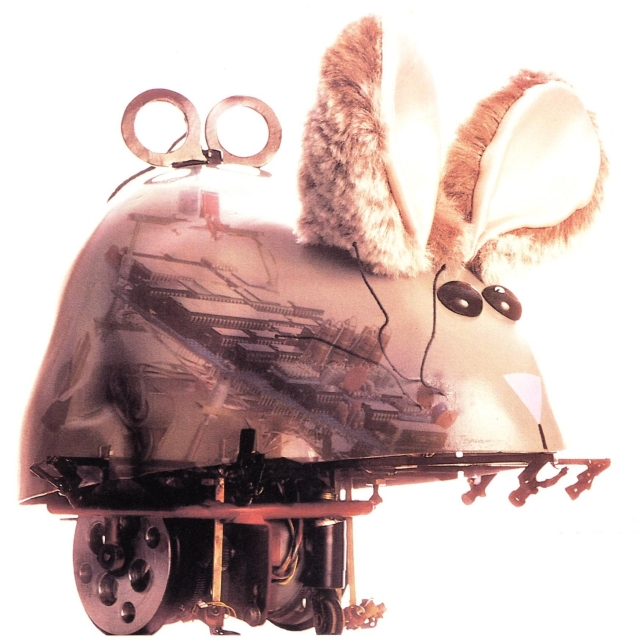
\includegraphics[width=0.6\textwidth]
	{Figures/MoonlightSpecial.jpg}
	\label{fig:MoonlightSpecial}
	\source{\citeonline{Moonlight2010}}
\end{figure}

\hspace{0.5cm} Sua ideia surge em 1977, quando a \textit{IEEE Spectrum Magazine} trouxe pela primeira vez o conceito de robôs autônomos para resolução de labirintos. Pouco tempo depois, sua primeira competição foi realizada, em junho de 1979, na primeira \textit{IEEE Amazing Micromouse Maze Contest} organizada na cidade de Nova York. Rapidamente, o conceito da competição se espalhou e, já no começo da década de 90, vários clubes voltados para Micromouse surgiam em escolas e universidades do mundo todo \cite{Tondr2004}.

\hspace{0.5cm} Atualmente, a \textit{IEEE Micromouse Competition} adota uma configuração que consiste em um labirinto de 16 x 16 blocos. Cada bloco possui 18 x 18 cm. As paredes, que possuem 5 cm de altura, são pintadas de branco de modo a ser reflexiva à luz infravermelha. O chão, por outro lado, é pintado de preto, para que não seja reflexivo. Além disso, os competidores sabem previamente que o \textit{micromouse} tem seu ponto de partida localizado em um dos cantos do labirintos, devendo alcançar o seu centro para terminar o desafio. Com base nisso, os participantes devem usar de algorítimos de busca para explorar o labirinto e encontrar a rota mais otimizada para o ponto de chegada estabelecido pela competição. O robô por sua vez, não pode ter suas dimensões maiores que uma seção de 25 x 25 cm. 
%As regras completas estão dispostas como anexo no final do documento.

%--------- NEW SECTION ----------------------
\section{Robótica e \textit{Frameworks}}
\label{sec:robotic_frameworks}
A palavra robô foi utilizada pela primeira vez em 1921 em uma peça teatral pelo dramaturgo checoslovaco Karel Capek. A origem vem da palavra checa robota que significa “trabalho forçado” e tornou-se popular através de filmes como Metrópolis (1926). O dia em que a terra parou (1951) e Planeta proibido (1956). Apesar da inserção do termo robô ser datada de 1921, registros históricos da antiga civilização grega já propunha o desenvolvimento dos primeiros modelos de robôs. Esses tinham aspecto visual semelhante ao de um humano e ou animal, e utilizavam sistemas de pesos e bombas pneumáticas, porém não tinham nenhuma funcionalidade prática, social, e como a época ainda não existia sistemas de produção complexos, esse robôs também não tinham função voltada à produtividade. Era um mecanismo de simples movimentação e sem nenhuma finalidade real. Algum tempo depois, cientistas árabes se dedicaram em fomentar a idéia e pesquisar sobre atribuir possíveis funções a esses robôs, com objetivo de facilitar as necessidades humanas. Esse pensamento revolucionário foi um grande marco na história da robótica. Segundo (PAPERT, 2008) citado por \citeonline {Mahmud2017}, documentos históricos datados de 1495 revelam que Leonardo Da Vinci ao desenvolver uma grande investigação sobre a anatomia humana, permitiu o desenvolvimento de exemplares de bonecos que obtinham articulações mecânicas, sendo capazes de mover as mãos, cabeça, olhos e pernas, conseguiam até realizar algumas ações mais simples, tal como, escrever ou tocar alguns instrumentos. 

O desenvolvimento produtivo em larga escala dos robôs aconteceu no início do século XVIII com a ascensão da revolução industrial. Segundo (SANTOS; MENEZES, 2005) citado por \citeonline{Mahmud2017}, a indústria têxtil utilizava teares mecânicos e com o contínuo avanço da revolução industrial, as fábricas começaram a substituir algumas tarefas mecanizadas por máquinas capazes de reproduzir automaticamente estas ações.Os anos 30 foram marcados no campo da robótica pela produção de um robô humanoide, denominado de Elektro, produzido pela empresa Westinghouse Electric Corporation. Elektro foi apresentado em 1939 e 1940 na World’s Fair,  uma feira de exposição internacional de produtos manufaturados. Segundo (SILVA, 2009) citado por \citeonline{Mahmud2017}, o termo “robótica” foi enunciado pela primeira vez em 1942 pelo cientista Isaac Asimov, em uma pequena história chamada “Runaround”. Asimov também publicou uma compilação de histórias em 1950 chamada “I Robot”, na qual ele propunha a existência de 3 leis fundamentais aplicadas à robótica, e, posteriormente ele adicionou mais uma, a lei zero. Essas leis são:

\begin{enumerate}
	\item Um robô não pode ferir um ser humano ou, por omissão, permitir que um ser humano sofra algum mal;
	\item Um robô deve obedecer as ordem que lhe sejam dadas por seres humanos, exceto nos casos em que tais ordens contrariem a primeira lei;
	\item Um robô deve proteger sua própria existência desde que tal proteção não entre em conflito com a primeira e segunda lei.
\end{enumerate}

zero.     Um robô não pode fazer mal à humanidade e nem por inação, permitir que ela sofra algum mal.

Porém, atualmente estas leis são interpretadas de uma perspectiva puramente ficcional, afinal, no tempo em que foram formuladas, não se tinha dimensão do desenvolvimento vertiginoso que iria ocorrer na área da robótica.

Apesar de que robôs industriais não se assemelham ao físico humano, ainda assim eles os substituem ao desempenhar tarefas nocivas para as pessoas. O conceito de robô industrial foi patenteado por George Devol, em 1954. O avanço tecnológico permitiu que os robôs passassem a desempenhar funções muito mais complexas e em várias esferas profissionais, por exemplo, indústria automotiva, nuclear, aplicação espacial, aplicação na medicina, em  ambientes adversos, onde a presença humana se torna difícil e até mesmo impossível.

Se tratando de avanço tecnológico, o campo de engenharia de software está ligado diretamente com o desenvolvimento dos robôs atualmente e umas das principais ferramentas de auxílio na programação dos mais diversos tipos de robôs, é o \textit{framework}. Um \textit{framework} pode ser conceituado de algumas formas.	 

Segundo Fayad et al. (1999) e Johnson \& Foote (1988), citado por \citeonline{Junior2006}, “um \textit{framework }é um conjunto de classes que constitui um projeto abstrato para a solução de uma família de problemas.”

Para Mattsson (1992, 2000), citado por \citeonline{Junior2006} “um \textit{framework} é uma arquitetura desenvolvida como objetivo de atingir máxima reutilização, representada como um conjunto de classes abstratas e concretas, com grande potencial de especialização.”
Já para Buschmann et al. (1996), Pree (1995) e Pinto (2000), citado por \citeonline{Junior2006} “um \textit{framework }é definido como um software parcialmente completo projetado para ser instanciado.”

Apesar de diferentes as definições encontradas nas literaturas elas não são contraditórias. A ideia de reutilização de softwares é fundamental para a definição de \textit{framework}, afinal uma ferramenta propõe a execução de uma tarefa de maneira mais prática e rápida. Uma comparação deixando claro as diferenças entre um \textit{framework }e uma biblioteca de classe, pode permitir um melhor entendimento sobre o tema. Numa biblioteca de classes, cada classe é única e independente das outras. Já em um \textit{framework}, as dependências/colaborações estão embutidas, conforme ilustrado na Figura \ref{fig:biblioteca_vs_framework}.

\begin{figure}[H]
	\centering
	\caption{Biblioteca x \textit{Framework}.}
	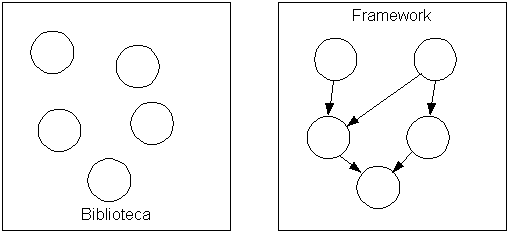
\includegraphics[width=0.7\textwidth]
	{Figures/biblioteca_vs_framework}
	\label{fig:biblioteca_vs_framework}
	\source{\citeonline{Sauve2001}}
\end{figure}

O \gls*{ros} é um exemplo de \textit{framework}. Ele é uma plataforma de software de código aberto, desenvolvido em 2007, projetado para suportar uma nova geração de robôs. A comunidade \gls*{ros} desenvolveu o \textit{framework} para várias plataformas, disponibilizando-os assim para diferentes \gls*{so}, como Windows, Linux e Mac OS. O \gls*{ros} é um conjunto de ferramentas que gerencia de forma eficiente  a mediação entre o SO e demais aplicações, possui uma estrutura flexível permitindo a criação de software de robôs. Detém uma coleção de bibliotecas e convenções com objetivo de simplificar tarefas complexas e criar estruturas mais robustas em uma ampla gama de plataformas robóticas. Pode-se afirmar que o \gls*{ros} representa uma coleção muito útil de softwares voltados exatamente para ajudar na percepção, controle e modelagem dos dispositivos de hardware que serão lidos, fornecendo serviços que são esperados de um SO, incluindo a abstração de hardware em baixo nível, o que permite a leitura e o controle do mesmo, passagem de mensagens entre processos e gerenciamento de pacotes (Quigley et al. 2009, apud \citeonline{Tavares2013}). O \gls*{ros} também disponibiliza ferramentas de aplicação de robótica nas áreas de navegação, simulação, visão, percepção e controle, sendo exemplo as bibliotecas de processamento de imagem (opencv, pcl) e simuladores (stage, gazebo).

Por ser uma plataforma com código aberto, o \gls*{ros} possui uma ampla documentação, bem detalhada, em sua maioria na língua inglesa. Na página da comunidade \gls*{ros}, existe um extenso material de apoio, oferecendo suporte a compartilhamento de códigos fonte e experiências realizadas com o \textit{framework}. A comunidade do \gls*{ros} permite que o usuário faça parte dela, mediante a um cadastro pessoal no site. Dessa forma, o usuário pode deixar eventuais perguntas e/ou dúvidas que poderão ajudá-lo a solucionar algum problema.

O framework \gls*{ros} foi projetado para atender a um conjunto específico de desafios encontrados durante o desenvolvimento de robôs. O \gls*{ros} é muito mais do que apenas um serviço oferecido a robôs móveis e de manipulação (Alexander et al. 2012, apud \citeonline{Tavares2013}).

O \gls*{ros} possui uma estrutura distribuída de processos, a qual apoia a reutilização de código em robótica. Suas bibliotecas possuem funcionalidade para diversas linguagens de programação, foi projetado com um idioma neutro, suportando C, C++, Python, LISP e Octave, apesar de que C++ e Python são as duas linguagens principais e com maior número de pacotes disponíveis. Além disso, O \gls*{ros} organiza seu conjunto de software em \textit{packages} ou pacotes em tradução livre. De acordo com o guia de utilização do \gls*{ros},

\begin{quoting}[rightmargin=0cm,leftmargin=4cm]
	\begin{singlespace}
		{\footnotesize
			[...]um pacote pode conter nós \gls*{ros}, uma biblioteca independente de \gls*{ros}, um conjunto de dados, arquivos de configuração, um software de terceiros ou qualquer outra coisa que constitua logicamente um módulo útil. O objetivo desses pacotes é fornecer essa funcionalidade útil de maneira fácil de consumir, para que o software possa ser facilmente reutilizado. Em geral, os pacotes \gls*{ros} seguem o princípio "Goldilocks": funcionalidade suficiente para ser útil, mas não muito que o pacote seja pesado e difícil de usar em outro software. \cite[tradução nossa]{rospackages}
		}
	\end{singlespace}
\end{quoting}


A comunicação do \gls*{ros} é baseada em eventos, utiliza processos para publicar/subscrever nós a tópicos. Conceitualiza-se que os nós publicam e subscrevem os tópicos, permitindo assim uma comunicação entre nós, onde recebem mensagens, apenas os que estiverem subscritos ao tópico.

A Figura \ref{fig:estrutura_comunicacao_ros} demonstra uma simples publicação e subscrição de dois nós a um tópico. Desta forma sempre que o nó publicar novas mensagens os nós que estejam subscritos ao tópico irão receber a informação.

\begin{figure}[H]
	\centering
	\caption{Estrutura de comunicação.}
	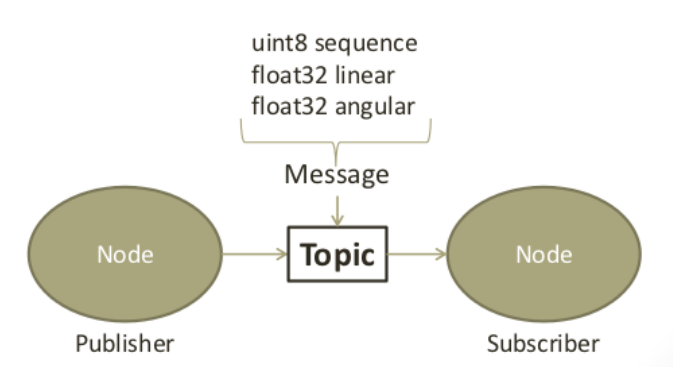
\includegraphics[width=0.7\textwidth]
	{Figures/estrutura_comunicacao_ros}
	\label{fig:estrutura_comunicacao_ros}
	\source{\citeonline{Santos2013}}
\end{figure}

Os nós correspondem à execução de um programa e são criados no sistema, geralmente, via console e sempre com o servidor mestre \gls*{ros} (roscore) iniciado. O servidor roscore é responsável por inicializar várias dependências, bibliotecas do \gls*{ros} e o sistema de comunicação entre nós. Devida as vantagens descritas neste tópico, será utilizado o \textit{framework} ROS para o desenvolvimento do Doogie Mouse.
%--------- NEW SECTION ----------------------
\section{Estudo do Estado da Arte}
\label{sec:sota}
Nessa seção, será realizado um estudo comparativo de alguns modelos de \textit{micromouse}, buscando avaliá-los sobre diferentes critérios a partir de uma matriz de comparação. O estudo auxiliou na realização do design da paltaforma proposta por esse trabalho uma vez que, através dele, verifica-se quais recursos são mais importantes para o comprimento dos requisitos do projeto, além de permitir um entendimento generalizado de como são feitos os robôs \textit{micromouse}. 

\subsection{GreenGiant}
A Green Giant é uma desenvolvedora de múltiplas plataformas de robótica, especializada em eletrônica embarcada, tendo como seu carro-chefe o \textit{micromouse}. Seu modelo mais recente, 2016 - 2017, é voltado para alto desempenho em competições, alcançando a posição de quarto lugar durante a \gls*{apec} de 2016.

\begin{figure}[H]
	\centering
	\caption{Robô Green Giant.}
	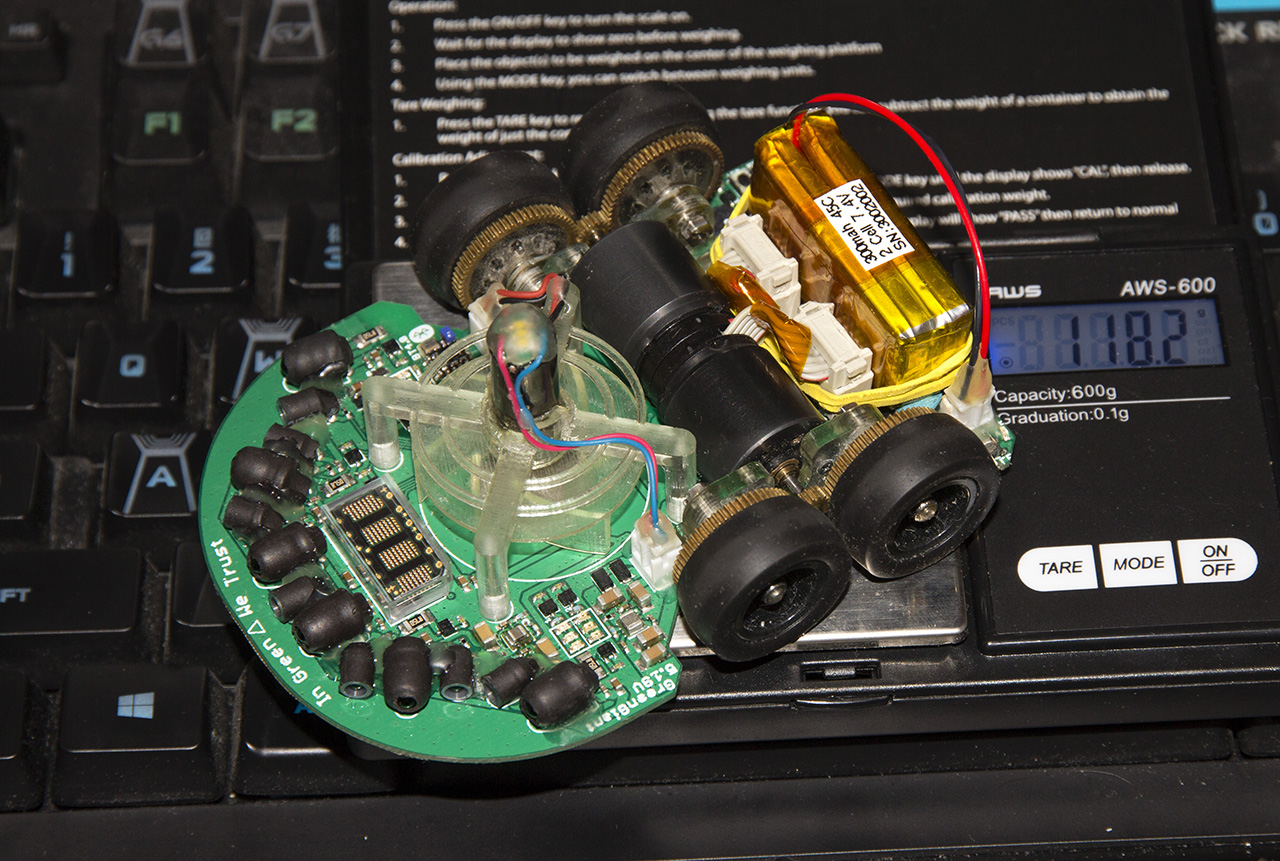
\includegraphics[width=0.7\textwidth]
	{Figures/GreenGiant_model.jpg}
	\label{fig:Green_Giant_model}
	\source{\citeonline{GreenGiant2016}}
	\end{figure}

Sua interface de usuário possui \textit{Dot Matrix Display}, sinalizadores LED, botões, buzzer, além de possuir um sistema de comunicação Bluetooth 4.0. Ademais, o modelo usa um sistema de ventoinhas de sucção para aumentar o nível de aderência das rodas, permitindo alcançar maiores velocidades sem derrapar.


\begin{table}[H]
	\centering
	\caption{Atributos do robô Green Giant}
	\label{tab:Green_Giant}
	\begin{tabular}{|l|l|}
		\hline
		\multicolumn{2}{|l|}{\textbf{Green Giant 5.19V}} \\ \hline
		Fabricante & Green Ye \\ \hline
		Ano & 2017 \\ \hline
		Linguagem de Programação & C/C++ \\ \hline
		Sensores & IR, MPU, IE \\ \hline
		Controlador & STM32 \\ \hline
		Simulador & - \\ \hline
		Bateria & LiPo 300mAh (7,4V) \\ \hline
		Rodas & 3D printed mount\&wheel + mini-z tyres \\ \hline
		Motor & DC-Motor 6.540RPM 0,21N.m (6V) \\ \hline
		User Interface & DMD 5x7, LEDs, Botão, Bluetooth \\ \hline
		Outros & sistema de ventoinhas de sucção \\ \hline
	\end{tabular}
	\source{Adaptado de \citeonline{GreenGiant2016}}
\end{table}


\textbf{Pontos Positivos:}
\begin{itemize}
	\item Produto de alto desempenho em competições;
	\item Sistema de ventoinhas de sucção.
\end{itemize}


\textbf{Pontos Negativos:}
\begin{itemize}
	\item Não possui suporte à simulação;
	\item Projeto pouco documentado;
	\item Não possui guia do usuário;
	\item Não possui suporte nativo para ambiente \gls*{ros}.
\end{itemize}


\subsection{WPISmartMouse}
A organização estudantil, WPI CollabLab, compartilham um espaço de laboratório entre seus membros para projetos com viez colaborativo a sociedade. Nesse espaço desenvolveu-se o Smartmouse, projeto \textit{micromouse} voltado para a competição Micromouse \textit{Brown IEEE Robotic  Olympiad}. O projeto também se extendeu para o desenvolvimento de um ambiente de simulação apartir dos projetos Gazebo e Ignition, não possuindo entretanto suporte para \gls*{ros}.

\begin{figure}[H]
	\centering
	\caption{Robô WPISmartMouse}
	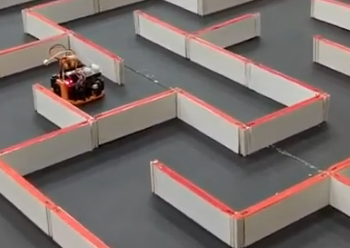
\includegraphics[width=0.5\textwidth]
	{Figures/WPISmartMouse_model.png}
	\label{fig:WPISmartMouse_model}
	\source{\citeonline{WpiSmartMouse2017}}
\end{figure}

\begin{table}[H]
	\centering
	\caption{Atributos do robô WPISmartmouse}
	\begin{tabular}{|l|l|}
		\hline
		\multicolumn{2}{|l|}{\textbf{Smartmouse}} \\ \hline
		Fabricante & WPI CollabLab \\ \hline
		Ano & 2018 \\ \hline
		Linguagem de Programação & Arduino/C, Python, BASCOM \\ \hline
		Sensores & IR, Magnetic Encoder \\ \hline
		Controlador & Teensy 3.6 \\ \hline
		Simulador & Gazebo \\ \hline
		Bateria & LiPo 1500mAh (7,4V) \\ \hline
		Rodas & Solarbotics RW2i Wheel \\ \hline
		Motor & DC-Motor 650RPM 2,35Nm(6V) \\ \hline
		User Interface & LEDs \\ \hline
		Outros & documentação no git \\ \hline
	\end{tabular}
	\label{tab:Smartmouse}
	\source{Adaptado de \citeonline{WpiSmartMouse2017}}
\end{table}

\textbf{Pontos Positivos:}
\begin{itemize}
	\item Provê ambiente de simulação;
	\item Documentação disponível no GitHub;
	\item Possui portabilidade para mais de uma linguagem de programação.
\end{itemize}

\textbf{Pontos Negativos:}
\begin{itemize}
	\item Não possui suporte nativo para ambiente \gls*{ros};
	\item Pouca variedade de sensores;
	\item Não possui guia do usuário;
	\item Poucos recursos na interface com o usuário.
\end{itemize}


\subsection{Kumamoto National College}
O Instituto Nacional de Tecnologia de Kumamoto, \textit{Kumamoto National College}, apresentou no ano de 2008 um projeto de desenvolvimento de ferramentas educacionais voltada para integração de sistemas e suas implementações. O projeto é direcionado aos seus estudantes do 5º ano de engenharia, através da produção de um \textit{micromouse} para a competição do ramo de \textit{Kyushu}.

\begin{figure}[H]
	\centering
	\caption{Robô Kumamoto.}
	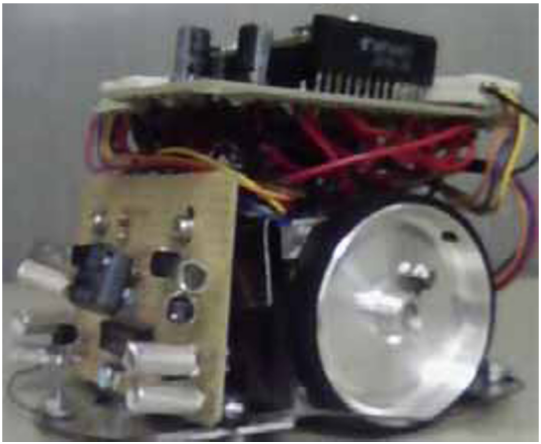
\includegraphics[width=0.5\textwidth]
	{Figures/Kumamoto_model.png}
	\label{fig:Kumamoto_model}
	\source{\citeonline{Kumamoto2010}}
\end{figure}

O hardware do robô foi bastante simplificado, visando facilitar o desenvolvimento pelos estudantes ainda não familiarizados com a robótica e eletrônica, além de buscar reduzir os custos de produção do robô. Como ferramenta educativa, o projeto conseguiu que seus estudantes produzissem o \textit{micromouse} em um semestre de atividades. Contudo, conceitos da robótica (ex: robótica móvel, fusão de sensores, visão, navegação) não foram trabalhados ou não foram citados no artigo gerado a partir do projeto.


\begin{table}[H]
	\centering
	\caption{Atributos do robô Kumamoto}
	\begin{tabular}{|l|l|}
		\hline
		\multicolumn{2}{|l|}{\textbf{Kumamoto National College}} \\ \hline
		Fabricante & Kiyoteru Hayama and Tsutomu Matsumoto \\ \hline
		Ano & 2008 \\ \hline
		Linguagem & C \\ \hline
		Sensores & IR \\ \hline
		Controlador & H8Tiny-3664 \\ \hline
		Simulador & - \\ \hline
		Bateria & LiPo 900mAh (7,4V) \\ \hline
		Rodas & wheels, tires \\ \hline
		Motor & Step Motor 0,78Nm (5,6V) \\ \hline
		User Interface & LEDs \\ \hline
		Outros & Documentação em artigo \\ \hline
	\end{tabular}
	\label{tab:Kumamoto}
	\source{Adaptado de \citeonline{Kumamoto2010}}
\end{table}



\textbf{Pontos Positivos:}
\begin{itemize}
	\item Projeto com fins educacionais;
	\item Fácil desenvolvimento.
\end{itemize}

\textbf{Pontos Negativos:}
\begin{itemize}
	\item Não possui suporte nativo para ambiente \gls*{ros};
	\item Pouca variedade de sensores;
	\item Não possui guia para usuário;
	\item Poucos recursos na interface com o usuário;
	\item Não possui nenhum ambiente de simulação.
\end{itemize}


\subsection{WolfieMouse}
\hspace{0.5cm} O WolfieMouse é um projeto de robótica que desenvolveu um \textit{micromouse} para competir na \textit{2018 Region 1 Robotics Competition}.

\begin{figure}[H]
	\centering
	\caption{Robô WolfieMouse.}
	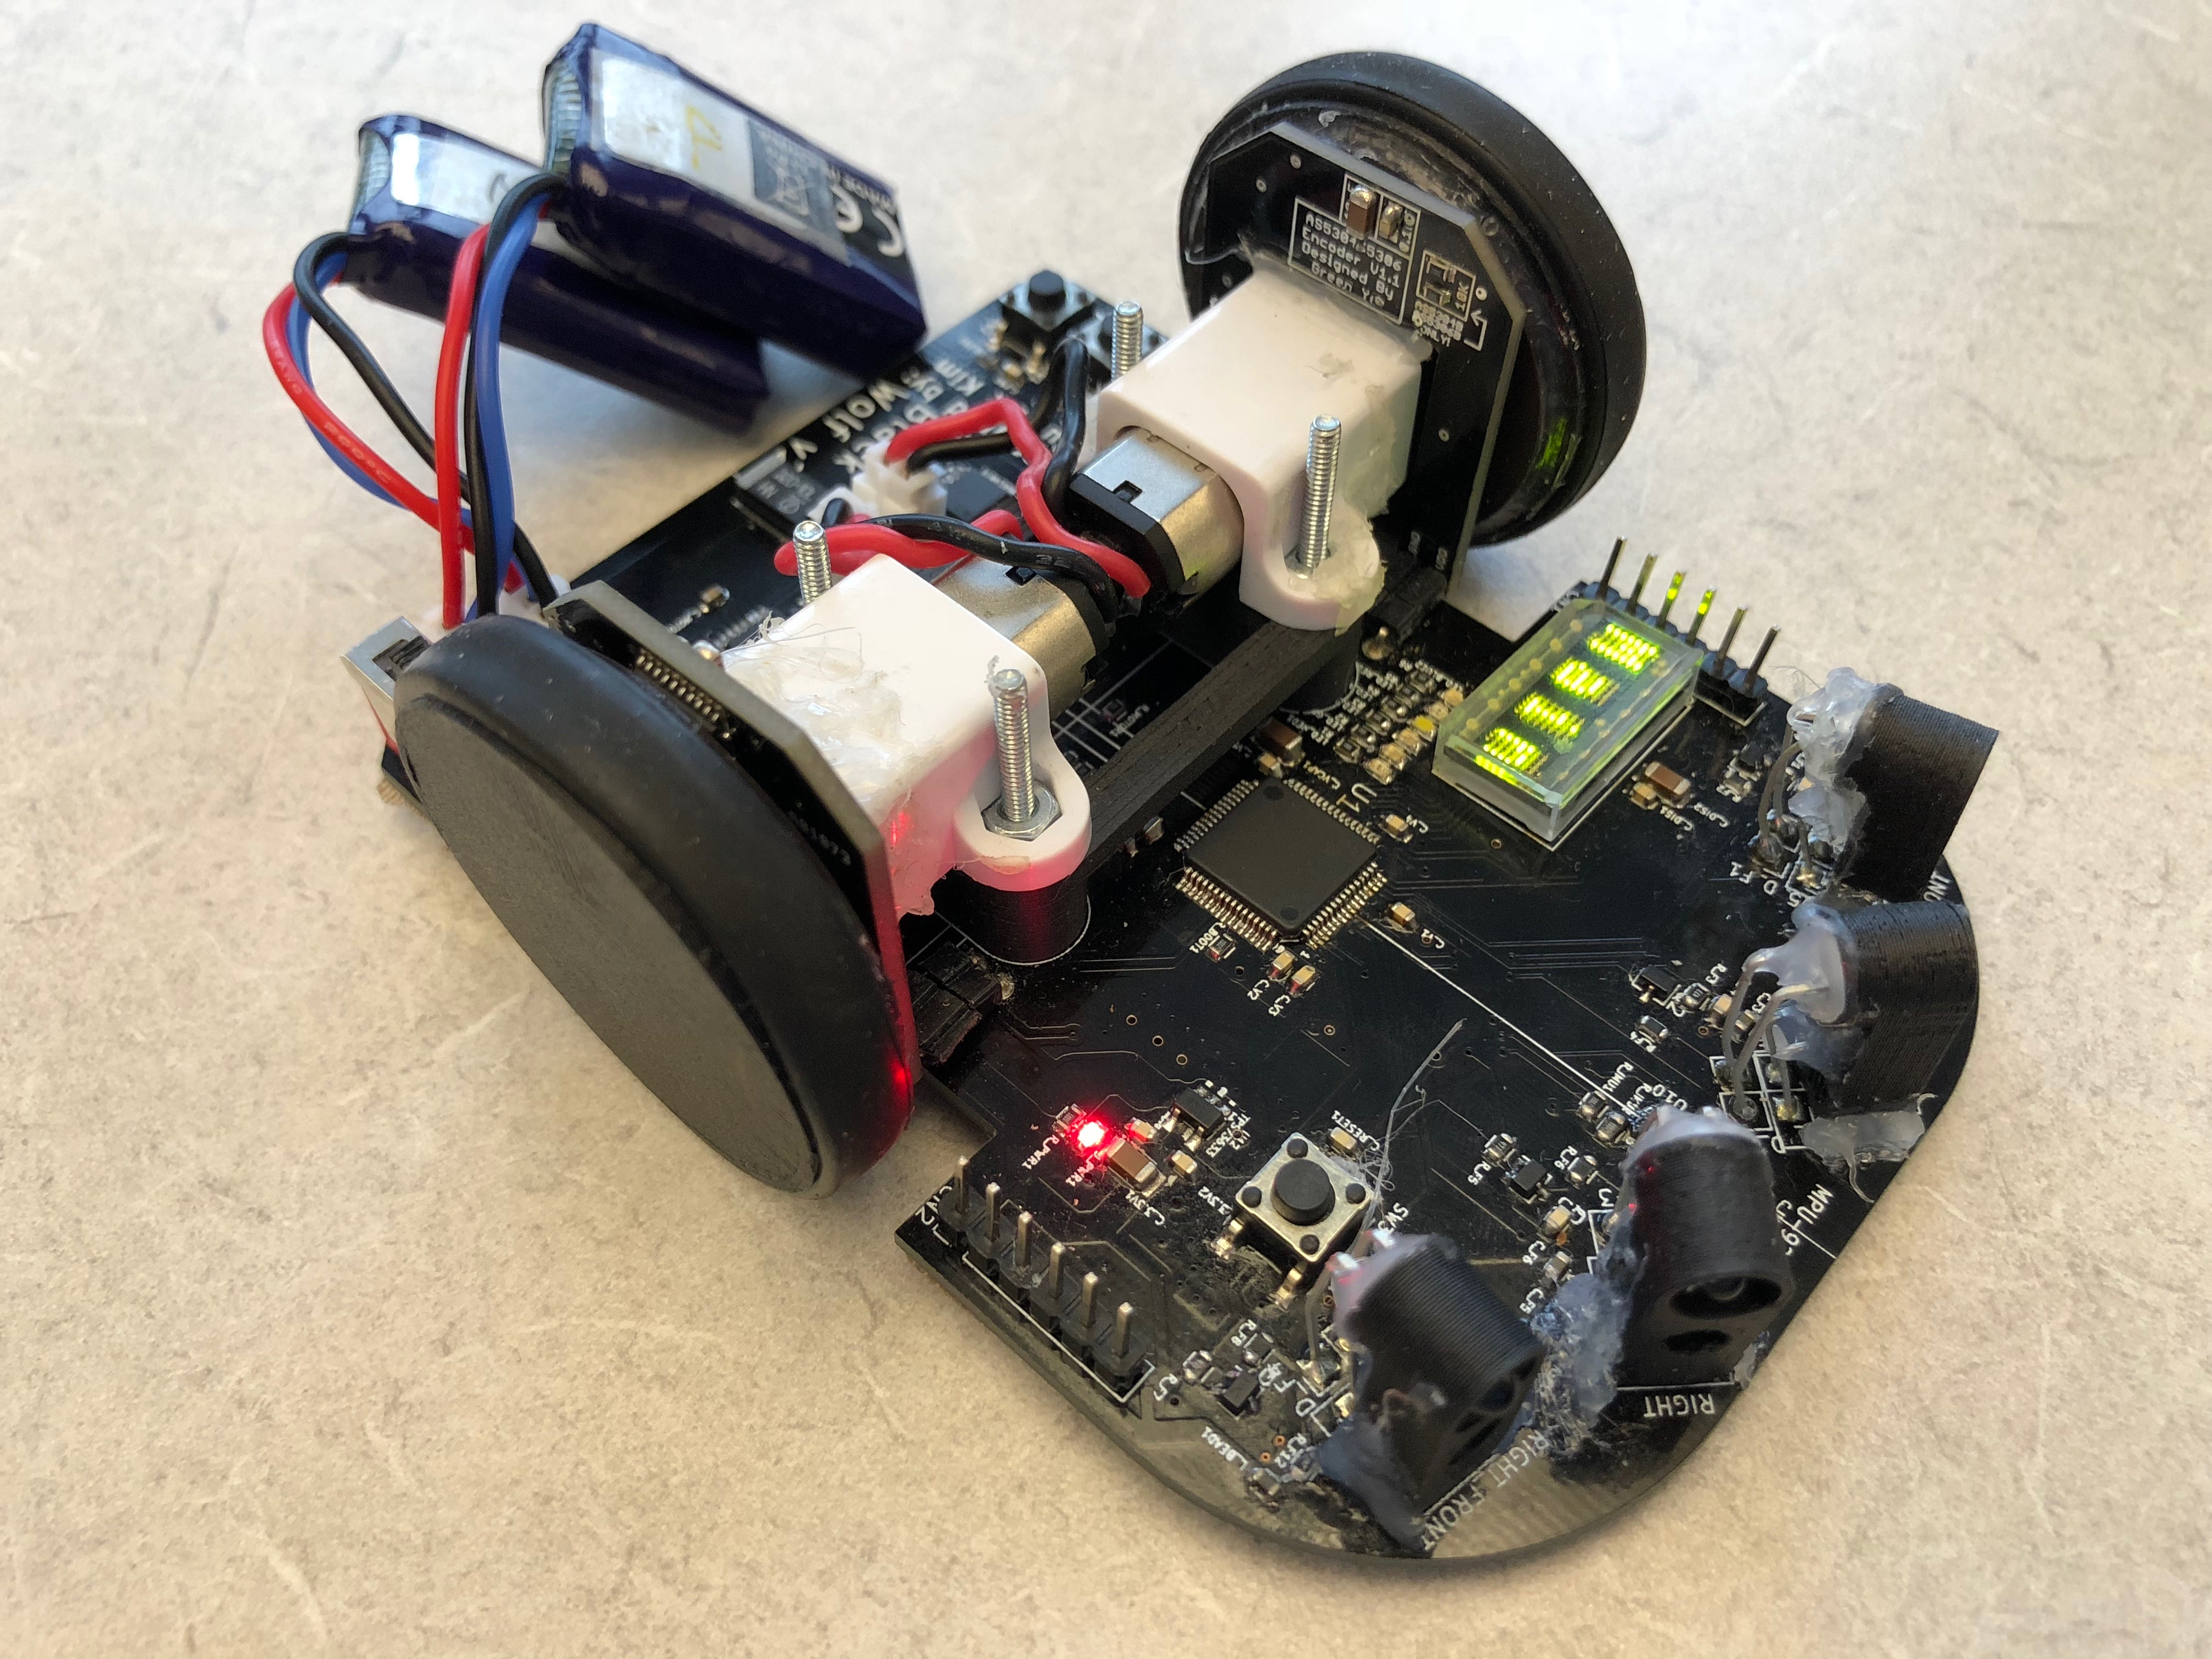
\includegraphics[width=0.7\textwidth]
	{Figures/WolfieMouse_model.jpg}
	\label{fig:WolfieMouse_model}
	\source{\citeonline{WolfieMouse2018}}
\end{figure}

Além da plataforma robótica, que conta com hardwares programados em baixo nível, para melhor otimização de seus controles, a equipe também realizou um ambiente de simulação baseado em C++ emulado no terminal do computador. Toda documentação foi disponibilizada em um repositório git, que também possui tutoriais para o desenvolvimento do robô.

\begin{table}[H]
	\centering
	\caption{Atributos do robô WolfieMouse}
	\begin{tabular}{|l|l|}
		\hline
		\multicolumn{2}{|l|}{\textbf{WolfieMouse}} \\ \hline
		Fabricante & Bryant Gonzaga, Bum Kim, Hyun Choi \\ \hline
		Ano & 2018 \\ \hline
		Linguagem & C++, C, ARM Assembly, Python \\ \hline
		Sensores & MPU, ToF, Magnetic Encoder \\ \hline
		Controlador & STM32 \\ \hline
		Simulador & Terminal-based \\ \hline
		Bateria & * \\ \hline
		Rodas & * \\ \hline
		Motor & DC-Motor \\ \hline
		User Interface & DMD 5x7, botões \\ \hline
		Outros & documentação e tutoriais no git \\ \hline
	\end{tabular}
	\label{tab:WolfieMouse}
	\source{Adaptado de \citeonline{WolfieMouse2018}}
\end{table}

\textbf{Pontos Positivos:}
\begin{itemize}
	\item Projeto bem documentado;
	\item Possui tutoriais;
	\item Possui ambiente de simulação.
\end{itemize}

\textbf{Pontos Negativos:}
\begin{itemize}
	\item Não possui suporte nativo para ambiente \gls*{ros};
	\item Pouco foco em finalidades educativas com o produto;
	\item Não possui guia para usuário;
	\item Poucos recursos na interface com o usuário.
\end{itemize}

\subsection{Raspberry Pi Mouse V2}
A RT Corporation Micromouse é uma desenvolvedora japonesa de plataformas robóticas voltada para aplicações  voltadas de pesquisas à hobistas. Um de seus segmentos é voltado para \textit{micromouse}, fortemente representado pelo seu produto Raspberry Pi Mouse V2, citado em "Learning ROS robot programming with Raspberry Pi" (Nikkei BP, June 2018).

\begin{figure}[H]
	\centering
	\caption{Robô RaspiMouse.}
	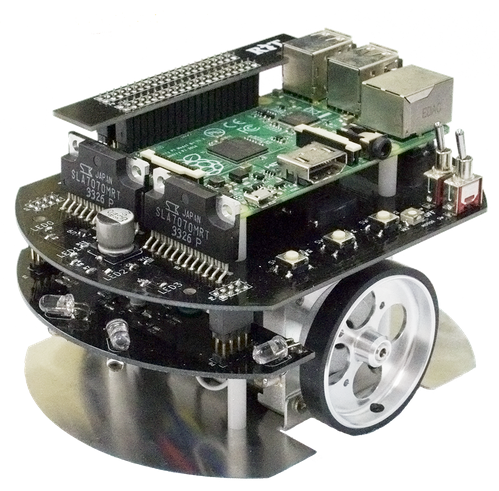
\includegraphics[width=0.5\textwidth]
	{Figures/RaspiMouse_model.png}
	\label{fig:RaspiMouse_model}
	\source{\citeonline{RaspiMouse2016}}
\end{figure}

O modelo citado, é um robô de plataforma baseado em \textit{micromouse} que utiliza uma Raspberry Pi como sua placa principal. Dessa forma o robô pode ser controlado pelos principais \textit{middleware} de robótica (ROS/RTM), possuindo inclusive pacotes publicados na wiki do \gls*{ros} voltados para navegação e simulação do \textit{micromouse};

\begin{table}[]
	\centering
	\caption{Atributos do robô RaspiMouse}
	\begin{tabular}{|l|l|}
		\hline
		\multicolumn{2}{|l|}{\textbf{Raspberry Pi Mouse V2}} \\ \hline
		Fabricante & RT Corporation \\ \hline
		Ano & 2016 \\ \hline
		Linguagem & Python, Shell \\ \hline
		Sensores & IR \\ \hline
		Controlador & RaspberryPi3 \\ \hline
		Simulador & Gazebo \\ \hline
		Bateria & LiPo 1000mAh (7,4V) \\ \hline
		Rodas & wheels, tires \\ \hline
		Motor & Step-Motor 400step/rev (4 fases) \\ \hline
		User Interface & Terminal, LEDs, Botão, Buzzer \\ \hline
		Outros & documentação no Git, mas em japonês \\ \hline
	\end{tabular}
	\label{tab:RaspiMouse}
	\source{Adaptado de \citeonline{RaspiMouse2016}}
\end{table}

\textbf{Pontos Positivos:}
\begin{itemize}
	\item Projeto bem documentado;
	\item Disponível no GitHub;
	\item Possui tutoriais;
	\item Possui ambiente de simulação;
	\item Suporte aos principais middleware de robótica (ROS/RTM);
	\item Possui pacotes do \gls*{ros} para seu controle;
	\item Plataforma é expansível.
\end{itemize}

\textbf{Pontos Negativos:}
\begin{itemize}
	\item Toda documentação do produto está em japonês;
	\item O robô é pouco compacto.
\end{itemize}

\subsection{Matriz de Comparação}

Através do estudo conforme tópico anteriores, montou-se uma matriz de comparação de forma a
quantificar atributos considerados mais significativos para o robô. Levou- se em conta, portanto, a existência da documentação disponível e seu nível de clareza; o uso de algum \textit{framework} de robótica; se faz uso ou suporta algum ambiente de simulação; diversidade de linguagens que a
plataforma pode ser programada; como é realizada a interface do usuário; quantidade de diferentes sensores e se a plataforma é expansível, podendo acrescentar a ela outros recursos (seja em hardware ou em software). Essa matriz pode ser visualizada no Apêndice \ref{apend:matriz_de_comparacao} deste documento.
    \chapter{Materiais e Métodos}
\label{chap:materiais_metodos}
O metodologia empregada nos trabalhos de conclusão de curso do Centro Universitário SENAI CIMATEC é executado com base na metodologia TheoPrax que foi desenvolvida pelo instituto Fraunhofer de Tecnologia Química, situado na Alemanha. A sistemática TheoPrax tem como principal objetivo incrementar a motivação da aprendizagem através do desenvolvimento de projetos reais voltados para empresas, proporcionando a integração entre o conhecimento técnico e sua aplicação prática. Para isto, esta estrutura envolve a identificação de uma situação problema ou de uma melhoria no processo ou no produto da empresa, seu estudo e, por fim, a definição de uma proposta técnica-financeira para implementação da solução.

\section{Metodologia}
\label{sec:metodologia}
A utilização da metodologia Theoprax se restringe apenas ao gerenciamento macro do projeto e não define como a solução proposta deve ser desenvolvida. Sendo assim, o desenvolvimento do projeto, proposto no tópico \ref{sec:objetivo_geral}, será realizado utilizando o procedimento ilustrado na figura \ref{fig:metodologia_diagrama} que foi adaptado da metodologia empregada no BIR (\textit{Brazilian Insitute of Robotics}) para desenvolvimento de projetos de robótica.

\begin{figure}[H]
	\centering
	\caption{Metodologia empregada no desenlvolvimento do projeto solução.}
	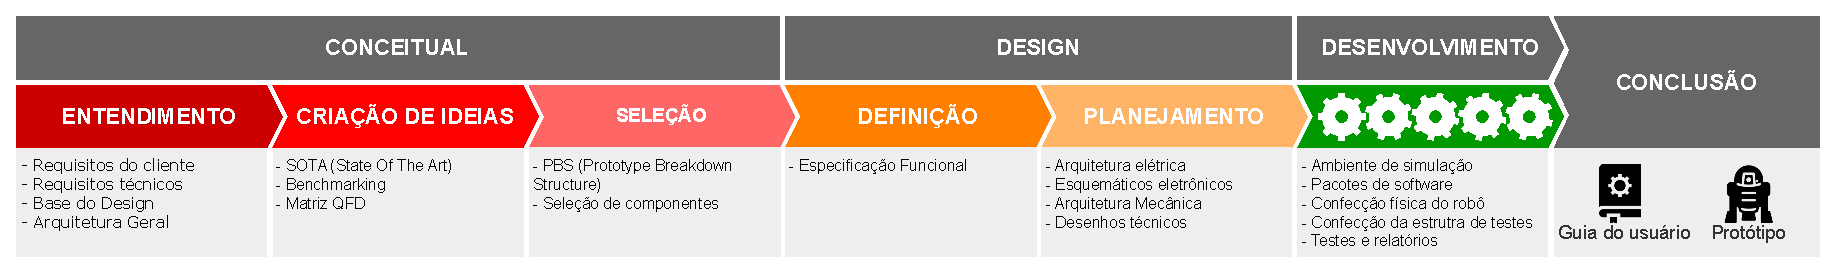
\includegraphics[width=1\textwidth]
	{Figures/metodologia_diagrama}
	\label{fig:metodologia_diagrama}
	\source{Própria Autoria}
\end{figure}	

Conforme Figura \ref{fig:metodologia_diagrama}, a metodologia utilizada neste projeto possui 4 etapas: Conceitual, Design, Desenvolvimento e Conclusão. Por conseguinte, cada etapa possui entradas e saídas, que vão se complementando ao longo do desenvolvimento do projeto, as quais serão explicadas nos tópicos seguintes.

\subsection{Conceitual}
\label{subsec:metodologia_conceitual}

A primeira etapa, designada como \textbf{Conceitual}, embora não explicitada no diagrama, possui como entradas as informações provenientes do cliente. Essas informações, tais como o problema proposto e os seus requisitos são utilizadas para o entendimento do projeto, servindo como ponto de partida para formulação da proposta de solução. Diante dessas informações, é possível definir os requisitos técnicos com base nos desejos do cliente (requisitos do cliente); a base do design, que consiste na definição do escopo e o que será necessário para desenvolver o projeto: meios, padrões e os principais componentes (hardware e software); e a arquiterura geral, que fornece uma visão macro de como será a interação entre o hardware e o software do robô. 

Após o entendimento do projeto, passa-se para a criação de ideias. Nesta subetapa, algumas pesquisas são realizadas para ajudar no processo de criatividade e evitar a reimplementação do que já existe no mercado. Assim, utiliza-se o SOTA (\textit{State Of The Art}), documento que aponta as principais pesquisas  e estudos sobre o tema do projeto, referenciando pesquisas acadêmicas já realizadas; e o Benchmarking, que é uma relação oriunda do mercado na qual aponta os competidores para o sistema projetado, incluindo para cada competidor critérios de avaliações importantes para o projeto. Finalizando a subetapa de criação de ideias, tem-se a Matriz QFD (\textit{Quality Functional Deployment}), em que os requisitos do cliente são confrontados com os requisitos técnicos, fornecendo à equipe de desenvolvimento do projeto os principais pontos que deverão receber maior atenção durante a elaboração do projeto. 

Por fim, após o entendimento do projeto e a formulação da ideia, parte-se para a etapa de seleção dos principais componentes do  sistema, em que primeiro elabora-se o PBS (\textit{Prototype Breakdown Structure}), uma representação do projeto com uma visão de subsistemas, apresentado através de um fluxo estruturado.

\subsection{Design}
\label{subsec:metodologia_design}
Com o conceito pré-estabelecido do sistema que será desenvolvido, parte-se para a etapa de \textbf{Design}. Nesta fase, define-se o sistema de maneira mais clara, tendo a especificação funcional como principal elemento. Este documento compreende a explicação  detalhada de cada funcionalidade do robô, contendo a definição, o objetivo, as premissas e as suas entradas e saídas. Devido ao nível de detalhes da especificação funcional, revisões em documentos anteriores, principalmente a arquitetura geral, são realizadas durante esta fase. 

No final da etapa de Design, começa-se o planejamento para o desenvolvimento técnico do projeto. Durante o planejamento é elaborado a arquitetura elétrica do robô (uma visão mais detalhada da arquitetura geral), descrevendo as formas de conexão e os protocolos de comunicação entre os elementos que compõem o sistema; os equemáticos eletrônicos, os quais são utilizados para confecção das PCIs (Placa de Circuito Impresso) que comporão o sistema; a arquitetura mecânica, apresentando os elementos mecânicos do robô; e por fim, os desenhos técnicos mecânicos, utilizados posteriormente para fabricação das peças do protótipo. 

Em conclusão, esta fase é de extrema importância, pois possibilita a geração de documentos que podem ser utilizados para a replicação do projeto. Além do mais, permite mais fluidez no desenvolvimento técnico do robô.

\subsection{Desenvolvimento}
\label{subsec:metodologia_desenvolvimento}

Após a finalização do planejamento, começa-se a etapa de \textbf{Desenvolvimento} do projeto, em que o conceito e as ideias provenientes das etapas anteriores tornam-se concretas. Nesta fase são desenvolvidos e documentados os pacotes de software, os quais englobam tanto a unidade de controle do robô quanto os \textit{drivers} dos sensores, atuadores e elementos de interação com usuário. Muito dos pacotes aqui desenvolvidos, usam a especificação funcional como guia. 

Para auxiliar no processso de desenvolvimento, um ambiente de simulação torna-se elemento vital. O ambiente de simulação permite que ideias sejam propostas e testadas sem a necessidade do uso da plataforma física, acelerando o processo de desenvolvimento num âmbito em que se possui diversas pessoas trabalhando no mesmo sistema. Não menos importante, os simuladores evitam que danos sejam causados ao robô em caso de má implementação de algum algoritmo. 

Entretanto, os ambientes de simulação não refletem completamente os aspectos físicos do mundo real. Diante disso, na fase de desenvolvimento torna-se necessário também a confecção de um ambiente real para testes. Com essa estrutura, também chamada de \textit{Mockup}, pode-se realizar testes para validar o que foi desenvolvido e produzir relatórios que podem ser entregues ao cliente  como forma de acompanhamento do desenvolvimento técnico do projeto.

\subsection{Conclusão}
\label{metodologia_conclusao}
O projeto é finalizado na etapa de \textbf{Conclusão}, em que a solução proposta é entregue ao cliente. Nesta entrega é realizado a demonstração do funcionamento do robô, utilizando um ambiente real. Também é cedido além da documentação elaborada ao longo do desenvolvimento do projeto, um documento em formato de Guia do Usuário contendo as instruções para manipulação e replicação do protótipo desenvolvido.

%--------- NEW SECTION ----------------------

\section{Requisitos do projeto}
\label{sec:requisitos_do_projeto}
Como mencionado no início deste capítulo, uma das etapas da metodologia TheoPrax envolve a identificação de uma situação problema. No projeto em questão, foi solicitado ao cliente os requisitos que o Doogie Mouse deveria cumprir. Entretanto, tais requisitos refletem a vontade do cliente de forma não técnica. Assim, a partir dos requisitos do cliente, foram levantados por parte da equipe de desenvolvimento os requisitos técnicos, os quais fornecem objetivos específicos que o projeto deve atingir. Por consequência, o cumprimento dos requisitos técnicos decorre na aprovação dos requisitos do cliente. Abaixo estão listados os requisitos do cliente e técnicos do Doogie Mouse de forma hierárquica, isto é, para cada requisito do cliente estão listados seus respectivos requisitos técnicos associado.

\begin{enumerate}
	\item Documentação de fácil acesso e entendimento:
	\begin{enumerate}
		\item Disponibilização de todo código desenvolvido no GitHub;
		
		\item Disponibilização guia do usuário como Wiki no GitHub;
		
		\item Disponibilização em um repositório no GitHub esquemáticos eletrônicos, desenhos técnicos mecânicos e seus respectivos arquivos para possível edição.
	\end{enumerate}
	
	\item Uso de um sistema microprocessado comercial:
	\begin{enumerate}
		\item Utilização de uma Raspberry Pi como sistema microprocessado;
	\end{enumerate}
	
	\item Interface intuitiva:
	\begin{enumerate}
		\item Permissão ao usuário acesso remoto do terminal do sistema operacional do robô;
		
		\item Visualização do mapa do Labirinto no RViz;
		
		\item Disponibilização de botões e display para interação com usuário na ausência de acesso remoto.
		
	\end{enumerate}
	
	\item Tutoriais na internet para entendimento do funcionamento do robô:
	\begin{enumerate}
		\item Desenvolvimento de tutorial na ROS Wiki com os primeiros passos com robô, explicando ao usuário comandos básicos de locomoção;
		
		\item Desenvolvimento de tutorial na ROS Wiki explicando ao usuário como implementar no robô seu próprio algoritmo de resolução de labirinto.
	\end{enumerate}
	
	\item Autonomia suficiente para utilização em ao menos duas aulas consecutivas:
	\begin{enumerate}
		\item Bateria recarregável;
		
		\item Autonomia superior a 1h40min.
	\end{enumerate}
	
	\item Uso de componentes de fácil manipulação e com facilidade de aquisição:
	\begin{enumerate}
		\item Uso de conectores polarizados;
		
		\item Utilização de padrão de cores para cabos de conexão;
		
		\item Especificação de componentes disponíveis no mercado nacional;
		
		\item Desenvolvimento de shield de interface entre a plataforma de processamento e os sensores e atuadores.
	\end{enumerate}
	
	\item Estrutura física compatível com as regras estabelecidas em competições do IEEE:
	\begin{enumerate}
		\item Dimensões do robô devem ser menores que 15 x 15 x 10 cm.
	\end{enumerate}
\end{enumerate}

Por fim, para a proporcionar a equipe de desenvolvimento um guia em relação a aplicação dos esforços para que os requisitos do cliente e técnico fossem atingidos, foi realizado uma confrontação de tais requisitos. Esta análise foi derivada de uma ferramenta comumente utilizada em desenvolvimento de produto, denominada matriz QFD (\textit{Quality Function Deployment}). A confrontação dos requisitos do projeto proposto pode ser visualizada no Apêndice \ref{apend:matriz_QFD}. Observa-se na linha 5 da matriz que o requisito técnico "Permissão ao usuário de acesso remoto do terminal do sistema operacional do robô" possui apenas uma relação forte com o requisito do cliente "Interface intuitiva". Por outro lado, "Dimensões do robô devem ser menores que 15 x 15 x 10 cm", na linha 16, possui 2 relações fracas, uma média e uma forte com diferentes requisitos do cliente. Portanto, essas associações funcionam como direcionadores de esforços e prioridades das tarefas desenvolvidas ao longo do projeto.

%--------- NEW SECTION ----------------------
\section{Descrição do sistema}
\label{sec:descricao_do_sistema}
O Doogie é um robô autônomo capaz de mapear um labirinto e descobrir qual o menor caminho do seu ponto de partida até um ponto de chegada. Sua arquitetura, ilustrada na Figura \ref{fig:arquitetura_geral}, pode ser dividida em três partes: interação com o usuário, controle do sistema e interface de hardware.
Para a interação com o usuário, o robô possuirá um Buzzer e dois \textit{Push Buttons}. Além disso, há a possibilidade de acessar o sistema do robô via SSH (\textit{Secure Shell}), por intermédio da conexão WiFi. A interface de hardware é composta por motores de corrente contínua, responsáveis pela movimentação, trabalhando em conjunto com uma ponte H e Encoders; sensores infravermelhos, dispostos na frente e dos lados, a fim de identificar paredes; e uma IMU (\textit{Inertial Measurement Unit}), responsável por fornecer a aceleração linear e a velocidade angular da plataforma móvel para complementar os dados de Odometria. O controle do sistema é embarcado dentro de uma Raspberry Pi Zero que utiliza o framework ROS para gerenciar os diversos subsistemas do micromouse.

\begin{figure}[H]
	\centering
	\caption{Arquitetura Geral do robô Doogie.}
	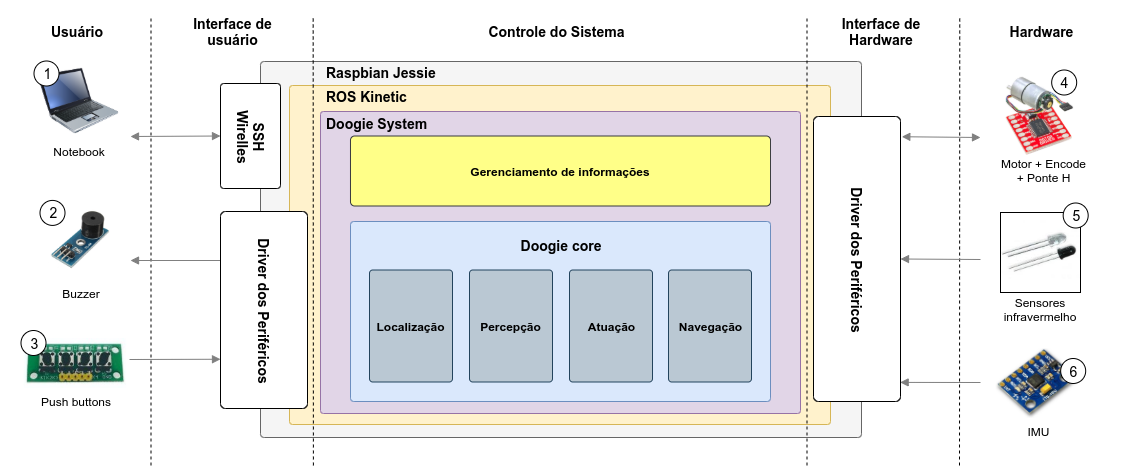
\includegraphics[width=1\textwidth]
	{Figures/arquitetura_geral}
	\label{fig:arquitetura_geral}
	\source{Própria Autoria}
\end{figure}

\subsection{Interface de usuário}
\label{ssec:interface_de_usuario}
O acesso à Raspberry Pi Zero é feito via SSH permitindo maior acessibilidade e segurança nos dados. O mesmo é feito remotamente através de conexão \textit{wireless}, possibilitando o acesso a linha de comandos da Raspberry bem como seu sistema de arquivos, de um outro computador.
 
O robô tem uma interface de interação com o usuário através de dois \textit{Push Buttons} e um \textit{Buzzer}. Os botões são utilizados para execução de tarefas tais como iniciar  e parar a execução da rotina principal do robô. O acesso a tais dispositivos é feito através do driver do periférico GPIO (\textit{General Purpose Input/Output}) que oferece APIs (\textit{Application Programming Interface}) nas linguagens de programação Pyhton e C++.

\subsection{Interface de Hardware}
\label{ssec:interface_de_hardware}
O deslocamento do robô utiliza 2 motores de corrente contínua, acoplados à Encoders, possibilitando a obtenção de informações de posição e velocidade, com objetivo de otimizar o controle e acionamento dos motores. Além disso, para permitir que os motores girem em ambas as direções, são utilizados circuitos de ponte H.
 
Os sensores infravermelho são responsáveis por identificar obstáculos no trajeto do robô. Eles são dispostos de modo que o micromouse possa indentificar as paredes do labirinto à sua direita, esquerda e frente. Também é necessário auxílio da IMU para obtenção de dados através dos sensores acelerômetro e giroscópio para estimar a posição com maior precisão. De forma similar a interface de usuário, serão utilizados drivers para estabelecer a comunicação entre o ambiente ROS e o hardware acima descrito.

\subsection{Controle do sistema}
\label{ssec:controle_do_sistema}
A Raspberry Pi Zero é um mini computador de baixo custo e fácil acesso, capaz de reunir diversas funcionalidades em uma única placa de tamanho reduzido.  No mesmo, está instalado o sistema operacional Raspbian Jessie, possibilitando a utilização do framework ROS, responsável por gerenciar os subsistemas do robô.

Os principais subsistemas desenvolvidos para o Doogie foram:
\begin{itemize}
	\item \textbf{Localização:} o labirinto pode ser modelado em uma matriz, geralmente de tamanho 16x16. Esse subsistema tem o objetivo de prover informações sobre em qual posição dessa matriz o robô se encontra (linha e coluna);
	
	\item \textbf{Percepção:} com a utilização dos sensores infravermelho, o robô pode identificar se há obstáculos ao seu redor. Esse subsistema é responsável por informar se há obstáculos na frente, direita e/ou esquerda do mesmo;
	
	\item \textbf{Planejamento:} há diversas formas de mapear e completar o labirinto. Utilizando as informações obtidas dos outros subsistemas (localização e percepção), é possível realizar o algoritmo especificado e tomar as decisões necessárias para a realização da atividade;
	
	\item \textbf{Navegação:} subsistema responsável por gerenciar as ações de navegação do robô, tais como: ir para frente, virar para direita ou esquerda, parar, dentre outros.
	
	\item \textbf{Gerenciamento de Informações:} é o subsistema responsável por receber comandos através dos botões situados no chassi do robô e fornecer o mapa do labirinto a medida em que ele é percorrido. 
\end{itemize}

%--------- NEW SECTION ----------------------
\section{Especificação dos componentes}
\label{sec:especificacao_dos_componentes}
O robô Doogie é capaz de realizar de forma autônoma a procura do melhor caminho do labirinto que leva-o ao ponto de chegada. Uma vez descoberto, o robô percorre esse percurso no menor tempo possível. Para isso, o robô é composto de um sistema microprocessado compatível com distribuições Linux; sensores de percepção que permitem a detecção de obstáculos ao redor do robô; sensores de posição para o controle dos movimentos e localização dentro do labirinto; atuadores para permitir a locomoção de forma autônoma. Além disso, ele é equipado com bateria recarregável, conversor analógico/digital, multiplexador analógico, botões, LEDs e Buzzer. Os tópicos seguintes irão detalhar os principais componentes da plataforma móvel.

\subsection{Raspiberry Pi Zero W v1.1}
\label{ssec:raspiberry_pi_zero}
Para que o robô realize a resolução do labirinto, é necessário que ele contenha uma unidade de processamento central. Este dispositivo tem como objetivo, a partir dos dados dos sensores e de um algoritmo de resolução de labirintos, inferir qual o melhor conjunto de movimentos que permita o robô alcançar o ponto de chegada do labirinto no menor tempo possível. Como o modelo de robô Micromouse possui um baixo nível de abstração de \textit{hardware}, é necessário também que a unidade de processamento disponibilize periféricos necessários para a comunicação com os componentes do sistema. Não menos importante, a unidade deve possuir compatibilidade com o \textit{framework} ROS, \textit{middleware }escolhido para o gerenciamento dos subsistemas que compõem o robô.

Portanto, foi escolhido o mini computador Raspberry PI Zero W v1.1: uma placa de baixo custo e com tamanho reduzido (apenas 6,5 x 3 cm), ótimo para projetos compactos como o robô Doogie. Esta placa é equipada com um processador \textit{single-core} Broadcom BCM2835 que opera na velocidade de 1 GHz aliado a uma memória RAM de 512 MB, além de um \textit{slot} para cartão microSD. A Raspberry PI Zero W v1.1 conta com \textit{WiFi} e \textit{Bluetooth} integrados, conector de vídeo mini HDMI e 2 portas USB para conectividade. Além disso, a placa permite que distribuições Linux como o Raspbian e Ubuntu sejam instaladas, as quais são compatíveis com \textit{framework} ROS. A Raspberry Pi oferece também APIs (\textit{Application Programming Interface}) nas linguagens de programação Pyhton e C++ para controle do seu periférico GPIO de 40 pinos. Essas interfaces permitem a utilização de protocolos de comunicação como UART, SPI e I2C; controle de motores através de saídas PWM; e pinos de entrada e saída para conexão com elementos digitais.

\subsection{Motor, Encoder e ponte H}
\label{ssec:motor_encoder_ponte-h}
Os robôs utilizados, em sua maioria, nas competições de Micromouse, têm como princípio de construção os robôs diferenciais. Este tipo de robô, muito comum no campo da robótica móvel, possui duas rodas conectadas a dois motores lateralmente opostos, os quais podem ser controlados independentemente. O sentido de giro e as velocidades das rodas determinam  o movimento do robô. Na especificação dos motores a serem utilizados em um robô diferencial, os parâmetros mais relevantes são sua velocidade e seu torque. Em casos de robôs providos por baterias, o consumo do motor e a tensão de alimentação são também fatores primordiais na sua escolha.

O controle utilizado em robôs diferenciais se baseia no modelo cinemático do mesmo, o qual inclui parâmetros construtivos dos robôs e, principalmente, as velocidades das rodas. Por isso, é necessário que além do motor, dois componentes estejam presentes na construção de um robô diferencial: um sensor de velocidade acoplado a cada roda, comumente utilizado um Encoder para tal função e um \textit{driver} de potência que permita controlar os motores de forma independente, isto é, controlar a velocidade e o sentido de giro de cada atuador.

Deste modo, o motor escolhido foi o \textit{Micro Metal Gearmotor HP 6V with Extended Motor Shaft} do fabricante Pololu. Para compatibilização, este fabricante fornece alguns componentes que podem ser comprados em conjunto com o motor. Assim, optou-se por utilizar o Encoder magnético desenvolvido para ser acoplado ao motor especificado, o qual possui uma resolução de 12 CPR (\textit{Count Per Revolution}) e faixa de operação de tensão entre 2,7 V até 18 V. Além do Encoder, foi utilizado o par de rodas de 32 x 7 mm e os elementos de fixação também disponibilizados pelo mesmo fabricante. As especificações técnicas do motor podem ser visualizadas na Tabela \ref{tab:especificacao_do_motor}

\begin{table}[H]
	\centering
	\captionsetup{justification=centering}
	\caption{Especificações técnicas do motor \textit{Micro Metal Gearmotor HP 6V with Extended Motor Shaft}}
	\label{tab:especificacao_do_motor}
	\begin{tabular}{c|c}
		\hline
		\textbf{Descrição} & \textbf{Valor} \\ \hline
		Tensão & 6 V \\ \hline
		Tamanho & 10 x 12 x 26 mm \\ \hline
		Peso & 9,5 g \\ \hline
		Diâmetro do eixo & 3 mm \\ \hline
		Relação de redução & 29,86:1 \\ \hline
		Velocidade sem carga & 1000 RPM \\ \hline
		Corrente sem carga & 0,07 A \\ \hline
		Corrente com eixo parado & 1,6 A \\ \hline
		Torque com eixo parado & 0,57 kg.cm \\ \hline
		Máxima potência de saída1 & 1,5 W \\ \hline
		Máxima eficiência & 41 \% \\ \hline
		Velocidade na máxima eficiência & 830 rpm \\ \hline
		Torque na máxima eficiência & 0,10 kg.cm \\ \hline
		Corrente na máxima eficiência & 0,36 A \\ \hline
		Potência de saída na máxima eficiência & 0,89 W \\ \hline
	\end{tabular}
\end{table}

Para a ponte H, foi escolhido o módulo TB6612FNG, o qual permite o controle independente de dois motores de corrente contínua operando com tensão entre 4,5 à 13,5 V e com valores de corrente de até 1 A por canal. Não menos importante, este driver possui tensão lógica de operação entre 2,7 à 5,5 V e 100 kHz como máxima frequência de PWM permitida.

\subsection{Emissor e fotorreceptor Infravermelho}
\label{ssec:emissor_e_fotoreceptor_ir}
Os robôs da modalidade micromouse têm como funcionalidade essencial a percepção. Para que o sistema que controla  o robô decida qual a melhor opção de movimento, é necessário primeiro que se conheça quais as possibilidades existentes. Quem fornece informações para que essas possibilidades sejam criadas é exatamente a funcionalidade de percepção. O princípio básico dessa funcionalidade  é informar, para cada célula do labirinto, quantas paredes circundam-a e onde estes obstáculos se encontram (Norte, Sul, Leste e Oeste).

De acordo com as regras estabelecidas nas competições reguladas pelo IEEE Região 9, os labirintos devem possuir cores específicas para os elementos que o compõe. Para as paredes do labirinto, a cor utilizada é a branca. A cor branca, quando comparada a cores mais frias, possui um alto valor de reflectância de luz cujo o comprimento de onda esteja dentro da faixa do infravermelho. (PROCURAR EMBASAMENTO). Os sensores mais indicados que se beneficiam dessa característica são aqueles em que há alteração de propriedades física quando exposto a luz infravermelha. Sendo assim, a utilização de LEDs que operam com espectros não visíveis, como o infravermelho, em conjunto com fototransistores, é uma ótima opção para equipar robôs da modalidade micromouse.

Portanto, para instrumentar o projeto em questão, optou-se pela utilização do LED IR333C do fabricante Everlight, o qual opera na região do infravermelho, permitindo a emissão de luz com comprimento de onda de $940 \pm 45$ nm e com potência de dissipação e corrente máxima iguais a 150 mW e 100 mA respectivamente, ambas à temperatura ambiente. Para o receptor infravermelho, especificou-se o fototransistor PT333-3B do mesmo fabricante Everlight. Este sensor opera na faixa de espectro entre 840 a 1100 nm, possuindo maior sensibilidade quando exposto a ondas com comprimento de onda igual a 940 nm. À temperatura ambiente, o PT333-3B pode dissipar até 75 mW e drenar no seu coletor valores de correntes até 20 mA. Ambos componentes possui tensão de operação compatível a utilizada no robô Doogie. Vale ressaltar que estes componentes podem ser substituídos por similares desde que as características física e elétrica mencionadas sejam compatíveis.

\subsection{IMU}
\label{ssec:imu}
Os labirintos utilizados nas competições oficiais de Micromouse são formados por células de 18 x 18 cm. A estrutura física do labirinto é igual a uma matriz cuja a dimensão é 16 x 16. Sendo assim, os robôs devem saber em qual célula do labirinto ele se encontra no momento para coletar algumas informações, utilizadas posteriormente para a sua movimentação e para a otimização da solução do labirinto. Uma técnica utilizada para obter a posição do robô dentro do labirinto é a de Odometria. Nesta estratégia, a partir das informações do Encoder e das dimensões das rodas utilizadas, estima-se a distância percorrida em um intervalo de tempo, entretanto, é uma técnica vulnerável a erros acumulativos. Uma forma utilizada para melhorar a precisão deste método é a incorporação de uma IMU (\textit{Inertial Measurement Unit}), as quais têm seus dados fundidos com os dados da Odometria, resultando em uma medição mais confiável.

Isto posto, o robô Doogie foi equipado com a MPU-6050. Este sensor permite medição de aceleração e velocidade angular nos 3 eixos cartesianos, totalizando 6 graus de liberdade (6DOF), com a medição de cada canal disponibilizada por conversores A/D (Analógico Digital) com resolução de 16 bits. Além disso, a MPU-6050 realiza medição de temperaturas entre -40 à 85 \textdegree C possui interface de comunicação I2C e pode operar com tensões entre 3 à 5 V. Por im, algumas bibliotecas são disponibilizadas pela comunidade \textit{open source} para comunicação com este dispositivo nas linguagens de programação Python e C++.

\subsection{Conversor Analógico/Digital e Multiplexador Analógico}
\label{conversor_multiplexador_analogico}
Como descrito no tópico \ref{ssec:raspiberry_pi_zero}, a Raspberry Pi Zero W v1.1 possui 40 pinos digitais. Entretanto, nenhum deles é habilitado para fazer conversão A/D (Analógica/Digital). Como os sensores infravermelho especificados (ver tópico \ref{ssec:emissor_e_fotoreceptor_ir}) fornecem valores analógicos de tensão em sua saída, é necessário o uso de um conversor externo. Além disso, robôs autônomos necessitam de verificação periódica da autonomia de sua bateria. Essa informação é também obtida de forma analógica. Logo, torna-se necessário que o Doogie Mouse seja equipado com um conversor A/D externo.

Mediante o exposto, foi selecionado o conversor ADS1115. Esse conversor funciona com tensões entre 2 à 5,5 V, e a tensão máxima nos pinos analógicos é igual à tensão de alimentação. Os pinos analógicos podem ser programados como 4 pinos independentes, ou dois canais diferenciais. Ademais, a interface de comunicação utilizada pelo ADS1115 é I2C.

O ADS1115 possui apenas 4 canais, entretanto, são necessários 5 canais: 4 para os sensores infravermelho e um para bateria. Para solucionar a carência de canais, foi especificado o multiplexador analógico 74HC4051. Esse módulo pode multiplexar até 8 canais, permitindo tensões de 2 à 10 V e frequência de até 170 MHz.

\subsection{Estrutura analítica do protótipo}
\label{ssec:pbs}
Para fornecer uma visão macro dos componentes que compõe o robô, foi elaborado um diagrama hierárquico, denominado PBS (\textit{Prototype Breakdown Structure}). Conforme Figura \ref{fig:pbs}, é possível visualizar a dependência entre os subsistemas e os componentes do robô. Além disso, diferente da Figura \ref{fig:arquitetura_geral}, esse diagrama oferece maior detalhamento dos elementos que estão relacionados a cada subsistema do robô.

\begin{figure}[H]
	\centering
	\caption{\textit{Prototype Breakdown Structure} do Doogie Mouse}
	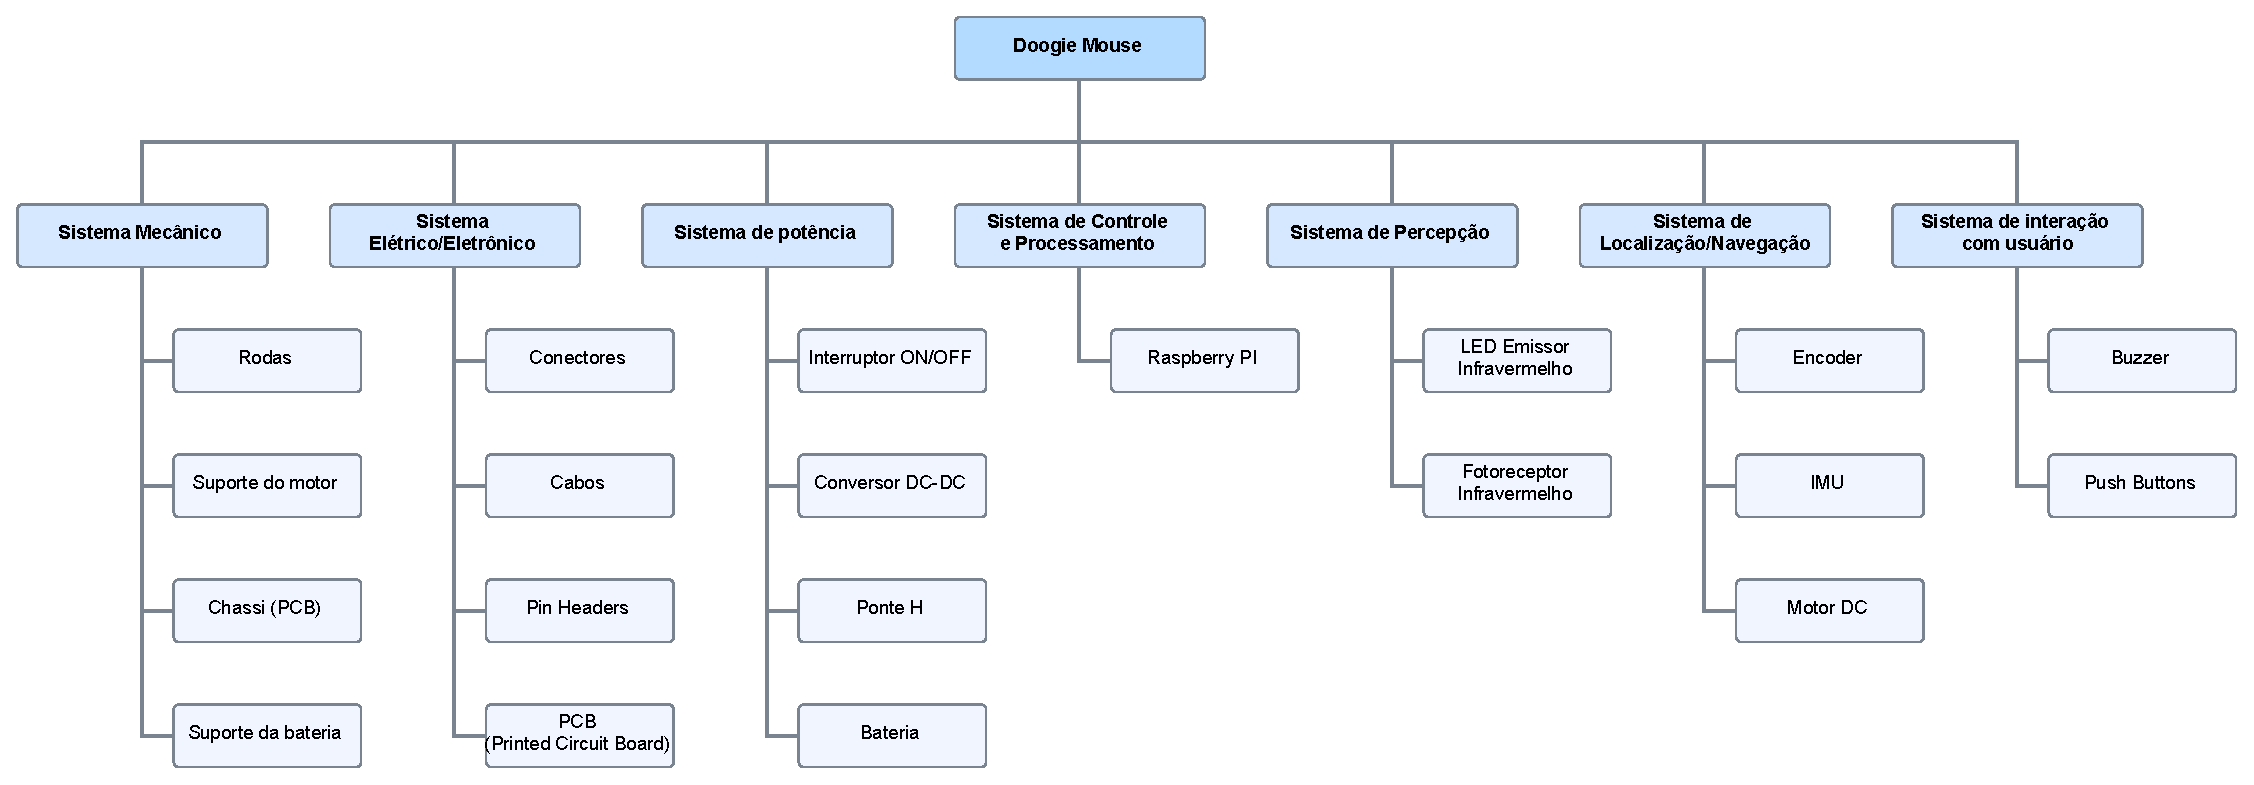
\includegraphics[width=1\textwidth]
	{Figures/prototype_breakdown_structure}
	\label{fig:pbs}
	\source{Própria Autoria}
\end{figure}

\subsection{Lista de componentes}
\label{ssec:bom}
A lista contendo todos os componentes bem como suas respectivas quantidades e descrição pode ser visualizada no Apêndice \ref{apend:bom} deste documento.

%--------- NEW SECTION ----------------------
\section{Modelo mecânico}
\label{sec:modelo_mecanico}
Para o design do robô, foi utilizado como um ponto de partida o TON-BOT v1.1, plataforma desenvolvida pela Ioton Technology \cite{ioton}. Além disso, conforme ítem 7 da subseção \ref{sec:requisitos_do_projeto}, ele deve ter suas dimensões não superiores à uma seção retangular de 15 x 15 x 10 cm.

A partir dessas premissas e da análise feita na subseção \ref{sec:requisitos_do_projeto}, buscou-se um design mecânico simples e de maior leveza. Dessa forma, foi utilizado como \textit{frame} do robô as próprias PCIs (Placa de Circuito Impresso), buscando posicionar suas rodas de forma a mantê-las alinhadas ao centro de massa de todo o conjunto mecânico. Para tanto, uma modelagem em CAD (\textit{Computer-Aided Design}) inicialmente foi realizada através da ferramenta Solidworks, buscando iterativamente a melhor disposição de seus elementos físicos (rodas, sensores e demais componentes eletrônicos das placas).  O modelo mecânico final pode ser visualizado na Figura \ref{fig:doogie_boards_3d}.

\begin{figure}[H]
	\centering
	\caption{Modelo 3D do Doogie Mouse}
	\subfigure[Representação 3D da placa inferior]{\label{fig:doogie_bottom__board_3d}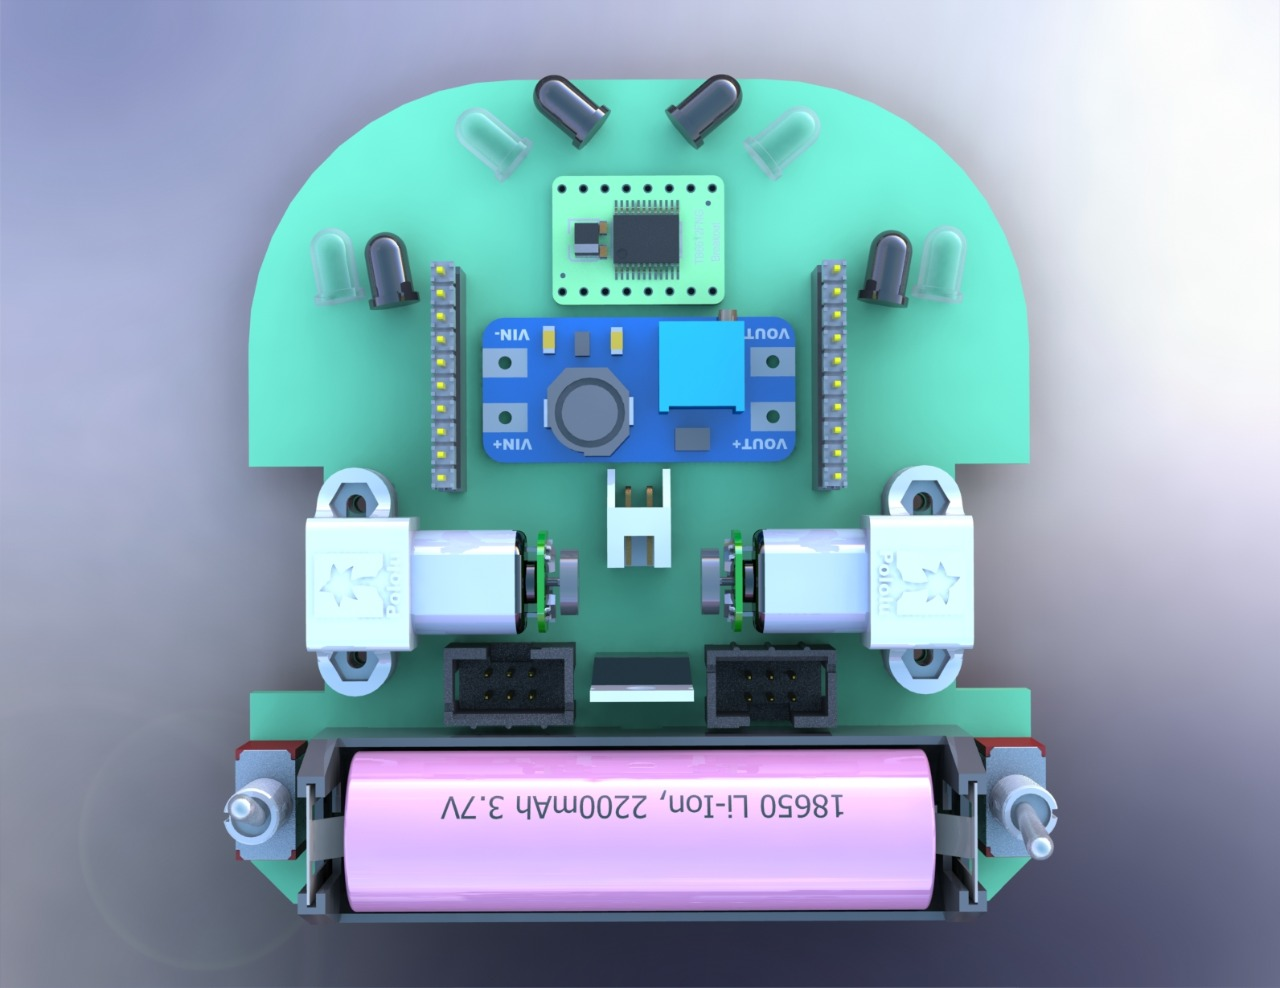
\includegraphics[scale=0.15]{doogie_bottom_board_3d.jpeg}}
	\subfigure[Representação 3D da placa superior]{\label{fig:doogie_top_board_3d}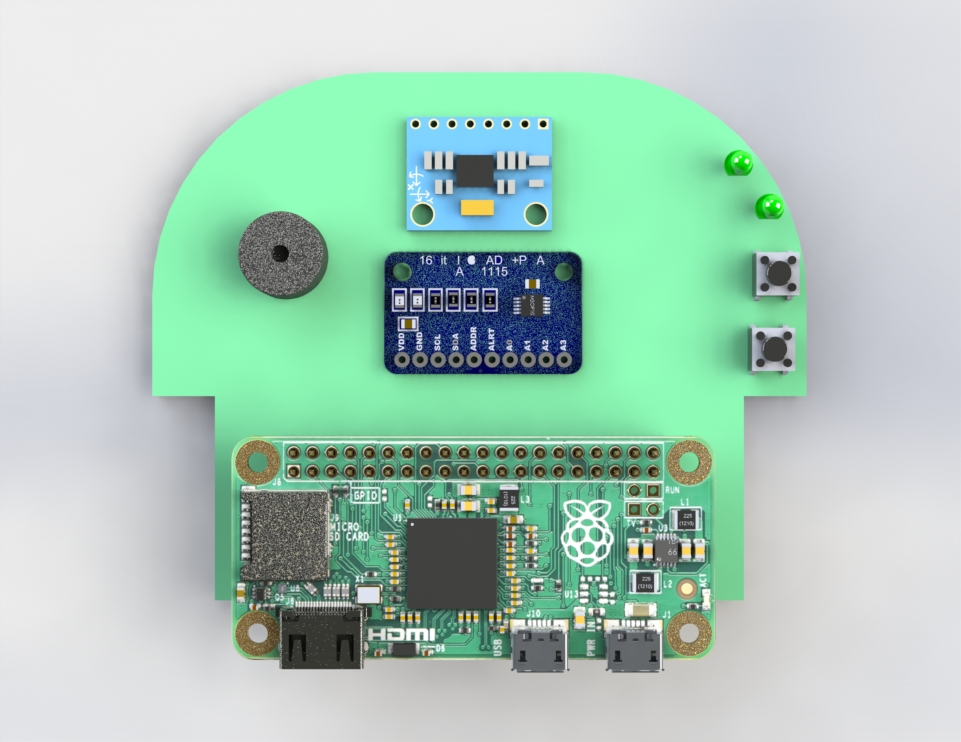
\includegraphics[scale=0.2]{doogie_top_board_3d.jpeg}}
	\subfigure[Modelo 3D do Doogie Mouse]{\label{fig:doogie_3d}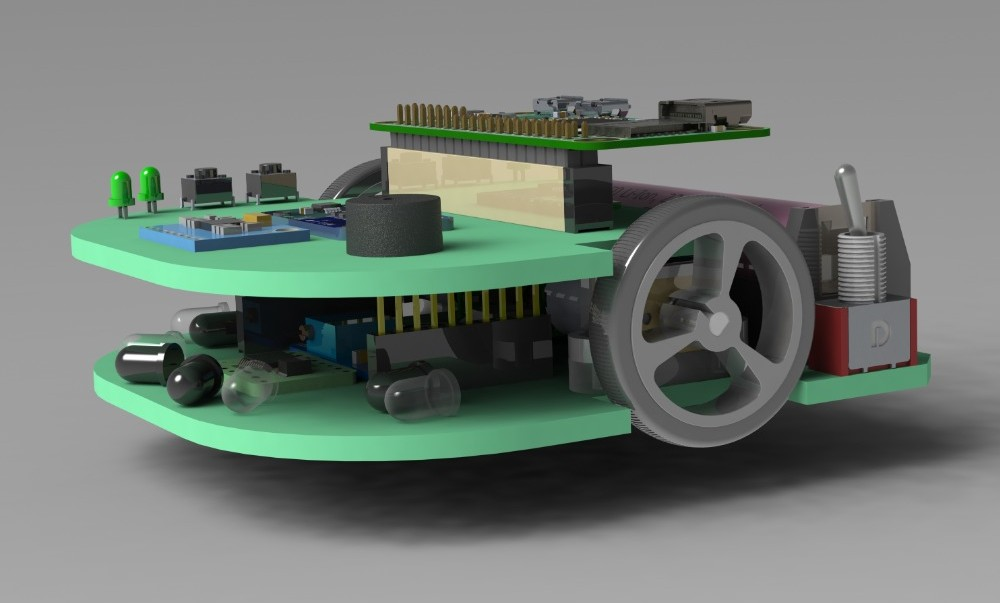
\includegraphics[scale=0.38]{doogie_3d.jpeg}}
	\label{fig:doogie_boards_3d}
\end{figure}

Da esquerda para direita visualiza-se as placas inferior, superior e o modelo completo do robô visto em perspectiva. A placa inferior possui 98 mm de comprimento e 92,90 mm de largura, enquanto a placa superior possui 75 mm de comprimento e 92,90 mm de largura. Foi necessário o uso de duas placas para melhor adequação dos componentes eletrônicos sem atrapalhar eventuais manutenções no dispositivo nem dificultar sua montagem.

\colorbox{yellow}{Referenciar desenhos técnicos em anexo}

%--------- NEW SECTION ----------------------
\section{Modelo esquemático de alimentação e comunicação}
\label{sec:arquitetura_eletrica_geral}
O Doogie é equipado com uma bateria do tipo Li-Ion com 3,6 V de tensão nominal. Para compatibilizar o nível de tensão da bateria com os demais componentes, são utilizados dois conversores DC-DC. O primeiro irá fornecer 6 V exclusivamente para os motores e os LEDs emissores. Já o segundo, é responsável por fornecer 5 V à Raspberry Pi. Entretanto, os componentes que estão conectados a Raspberry Pi são energizados com 3,3 V através de um conversor DC-DC interno a placa do sistema microprocessado.

Com intuito de facilitar a replicação do robô por usuários que queiram utilizá-lo, optou-se pelo uso de \textit{breakout boards}, que são placas eletrônicas pré-montadas. O Doogie possui seis delas: dois conversores de tensão DC-DC, um conversor Analógico/Digital (A/D), uma IMU, um multiplexador analógico e uma ponte H. Os demais componentes como resistores, transistores, LEDs infravermelho, fototransistores e conectores, são soldados diretamente na Placa de Circuito Impresso (PCI).

Os componentes do Doogie se comunicam e são controlados de diversas formas. O conversor A/D e a IMU se comunicam com a Raspberry Pi através de um barramento I2C. Como o conversor A/D especificado possui apenas 4 canais (um para cada sensor infravermelho), optou-se por utilizar um multiplexador analógico para permitir que o valor de tensão da bateria também seja obtido. Este multiplexador é controlado por pinos digitais da unidade de processamento. Por fim, o controle dos motores é realizado por uma ponte H com dois canais independentes. Esse \textit{driver} de potência permite que os sentidos de giros dos motores sejam controlados por pinos digitais da Raspberry Pi enquanto o controle de velocidade seja realizado por PWM (\textit{Pulse Width Modulation}).

A arquitetura elétrica na Figura \ref{fig:arquitetura_eletrica} demonstra como esses componentes descritos estão interligados eletricamente. A propósito de melhor visualização, o referencial de tensão (Ground - GND) foi omitido.

\begin{figure}[H]
	\centering
	\caption{Representação elétrica do Doogie Mouse.}
	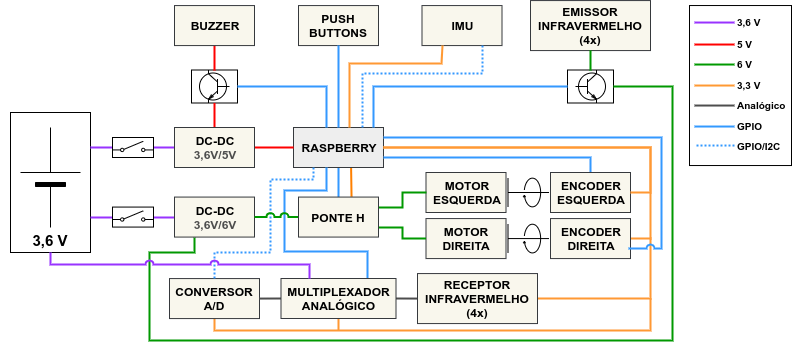
\includegraphics[width=1\textwidth]
	{Figures/arquitetura_eletrica}
	\label{fig:arquitetura_eletrica}
	\source{Própria Autoria}
\end{figure}

\subsection{Esquemáticos eletrônicos}
\label{ssec:esquematicos_eletronicos}
Como explicado no tópico \ref{sec:modelo_mecanico} o Doogie Mouse possui duas PCIs que são utilizadas como chassi do robô. Além disso, como também citado na subseção \ref{sec:arquitetura_eletrica_geral}, os componentes eletrônicos e as \textit{breakout boards} são soldados diretamente na PCI. Para elaboração do \textit{layout} de tais placas, foi utilizado o software Autodesk Eagle 9.4.2. O resutado obtido pode ser visualizado na Figura \ref{fig:doogie_boards}. Já os esquemáticos eletrônicos, que descrevem em maior detalhe as ligações elétricas entre todos os componentes do robô bem como o valor das grandezas físicas dos elementos eletrônicos, podem ser visualizados no Apêndice \ref{apend:diagramas_eletronicos} deste documento.

\begin{figure}[H]
	\centering
	\caption{\textit{Layout} das PCIs do Doogie Mouse}
	\subfigure[Placa inferior]{\label{fig:doogie_bottom_board}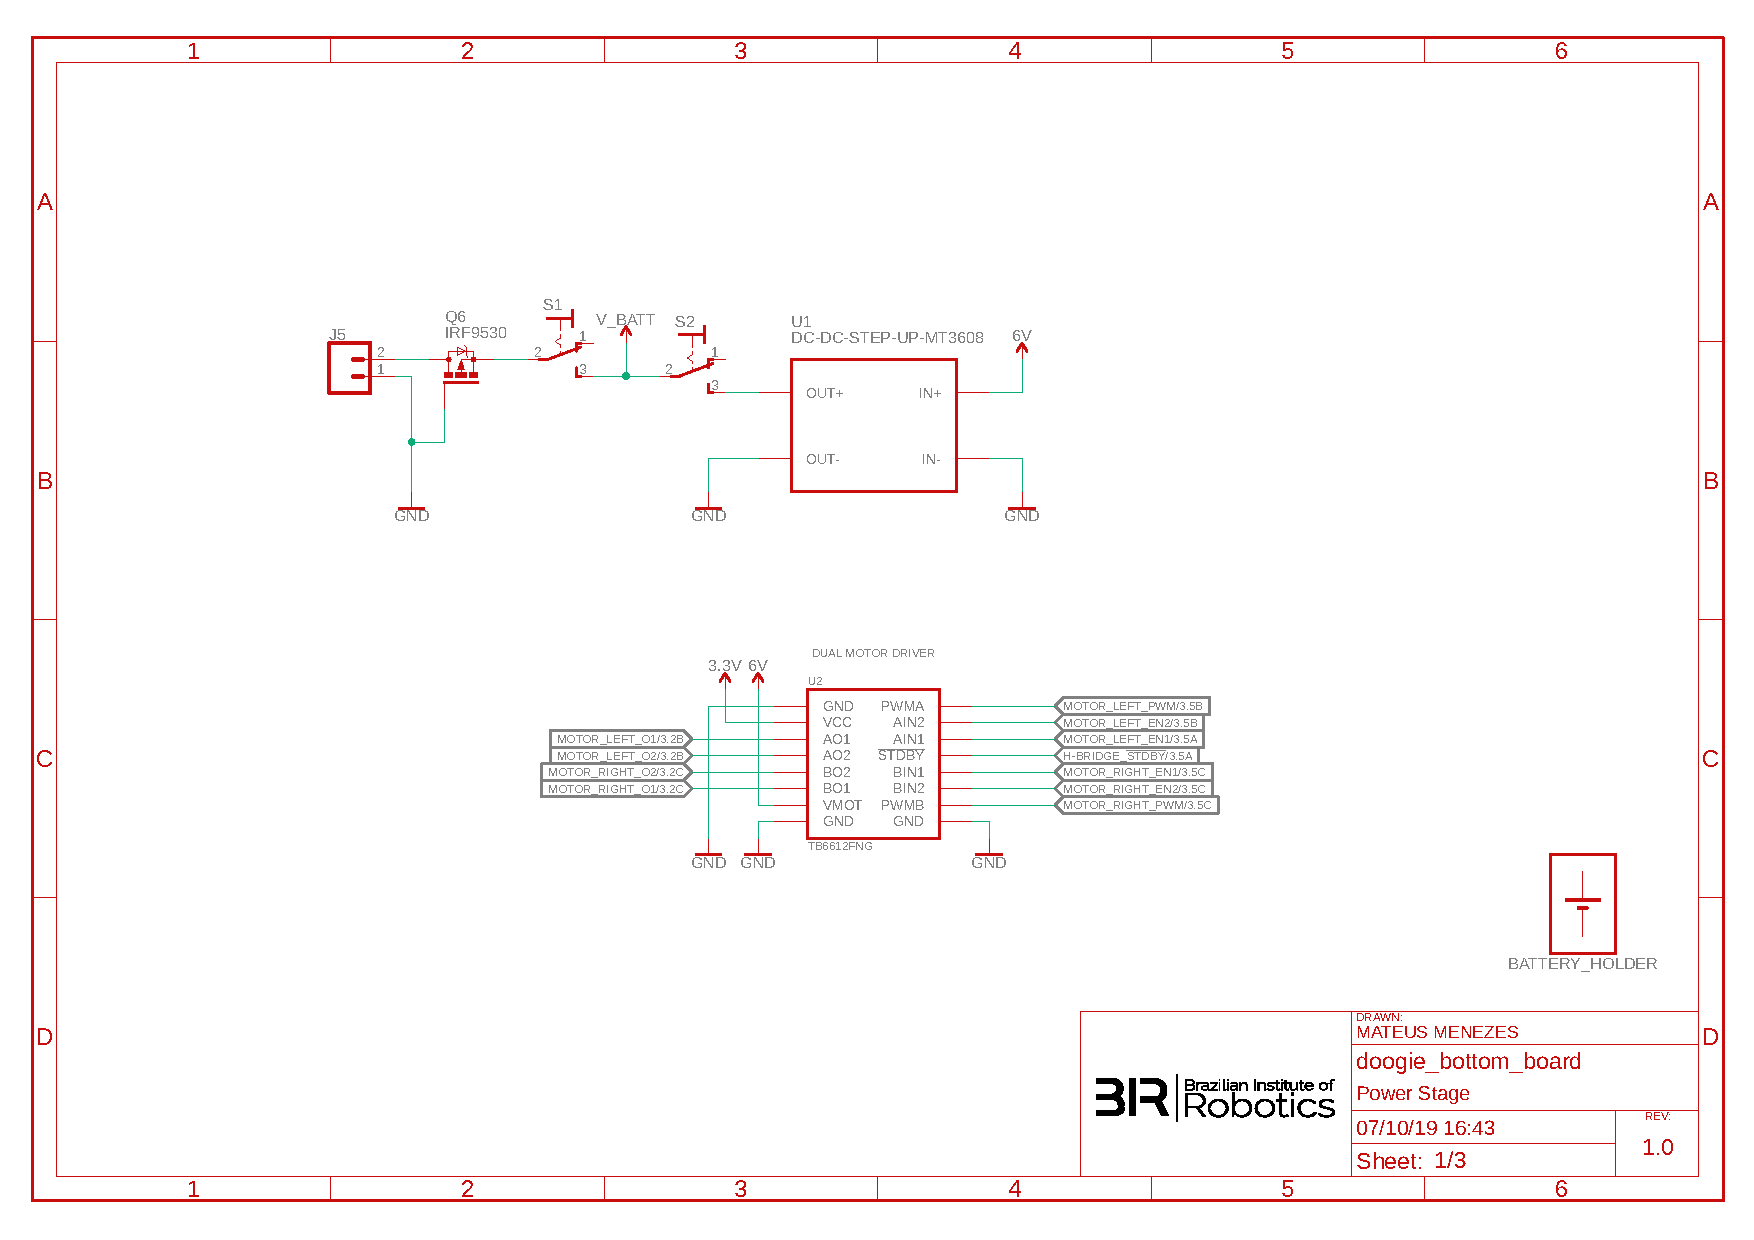
\includegraphics[scale=0.2]{doogie_bottom_board}}
	\subfigure[Placa superior]{\label{fig:doogie_top_board}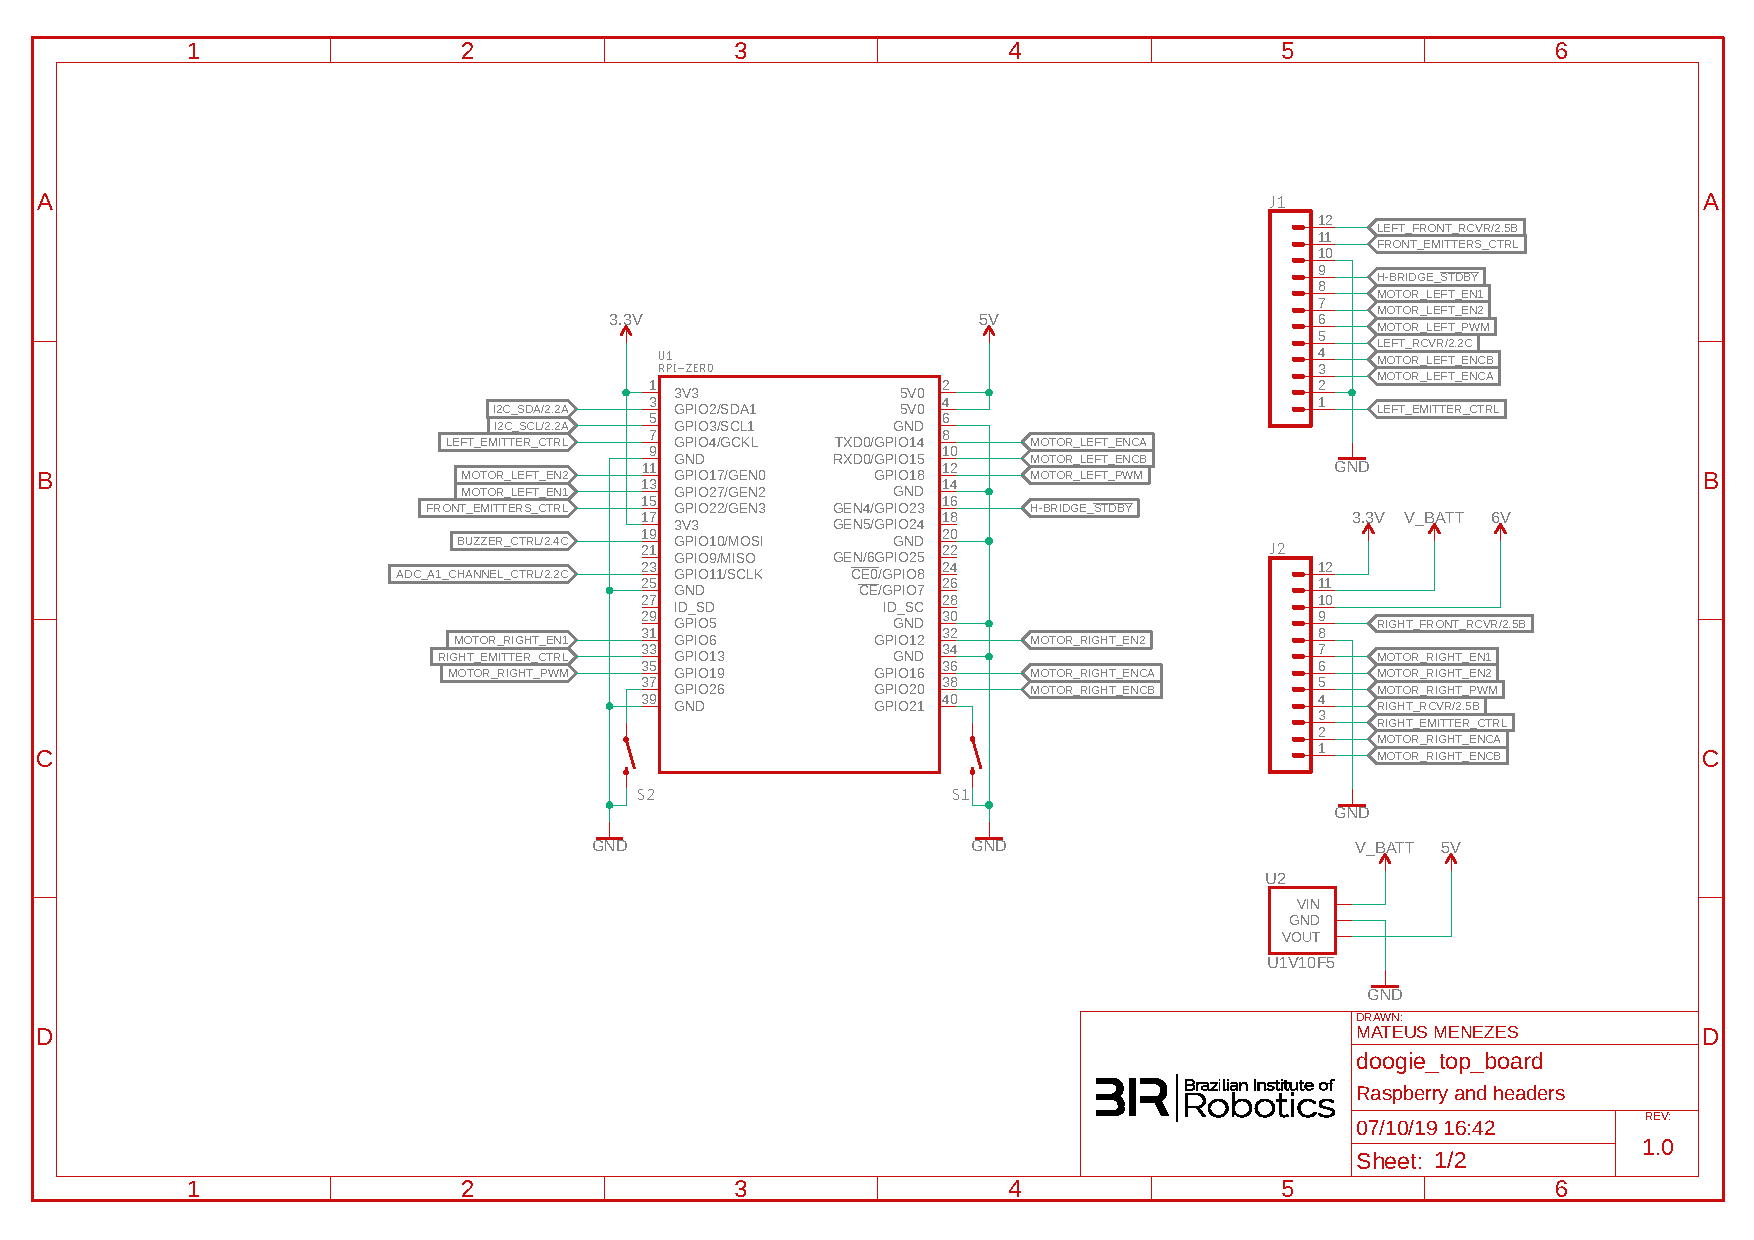
\includegraphics[scale=0.15]{doogie_top_board}}
	\label{fig:doogie_boards}
	\source{Própria Autoria}
\end{figure}

%--------- NEW SECTION ----------------------
\section{Especificação das funcionalidades}
\label{sec:especificacao_das_funcionalidades}
As funcionalidades de um robô descrevem os subsistemas e a lógica de operação dos mesmos. No Doogie, existem quatro funcionalidades principais: Localização, Percepção, Navegação e Usabilidade. O fluxo de informações de tais funcionalidades pode ser visualizado na Figura \ref{fig:especificacao_funcional_geral}. Observa-se nesse fluxograma como cada funcionalidade está interligada com as demais e quais informações são trafegadas entre elas. Para melhor entendimento, é descrito nos tópicos sequentes cada funcionalidade individualmente.

\begin{figure}[H]
	\centering
	\captionsetup{justification=centering}
	\caption{Fluxo de informações das funcionalidades Localização, Percepção, Navegação e Usabilidade.}
	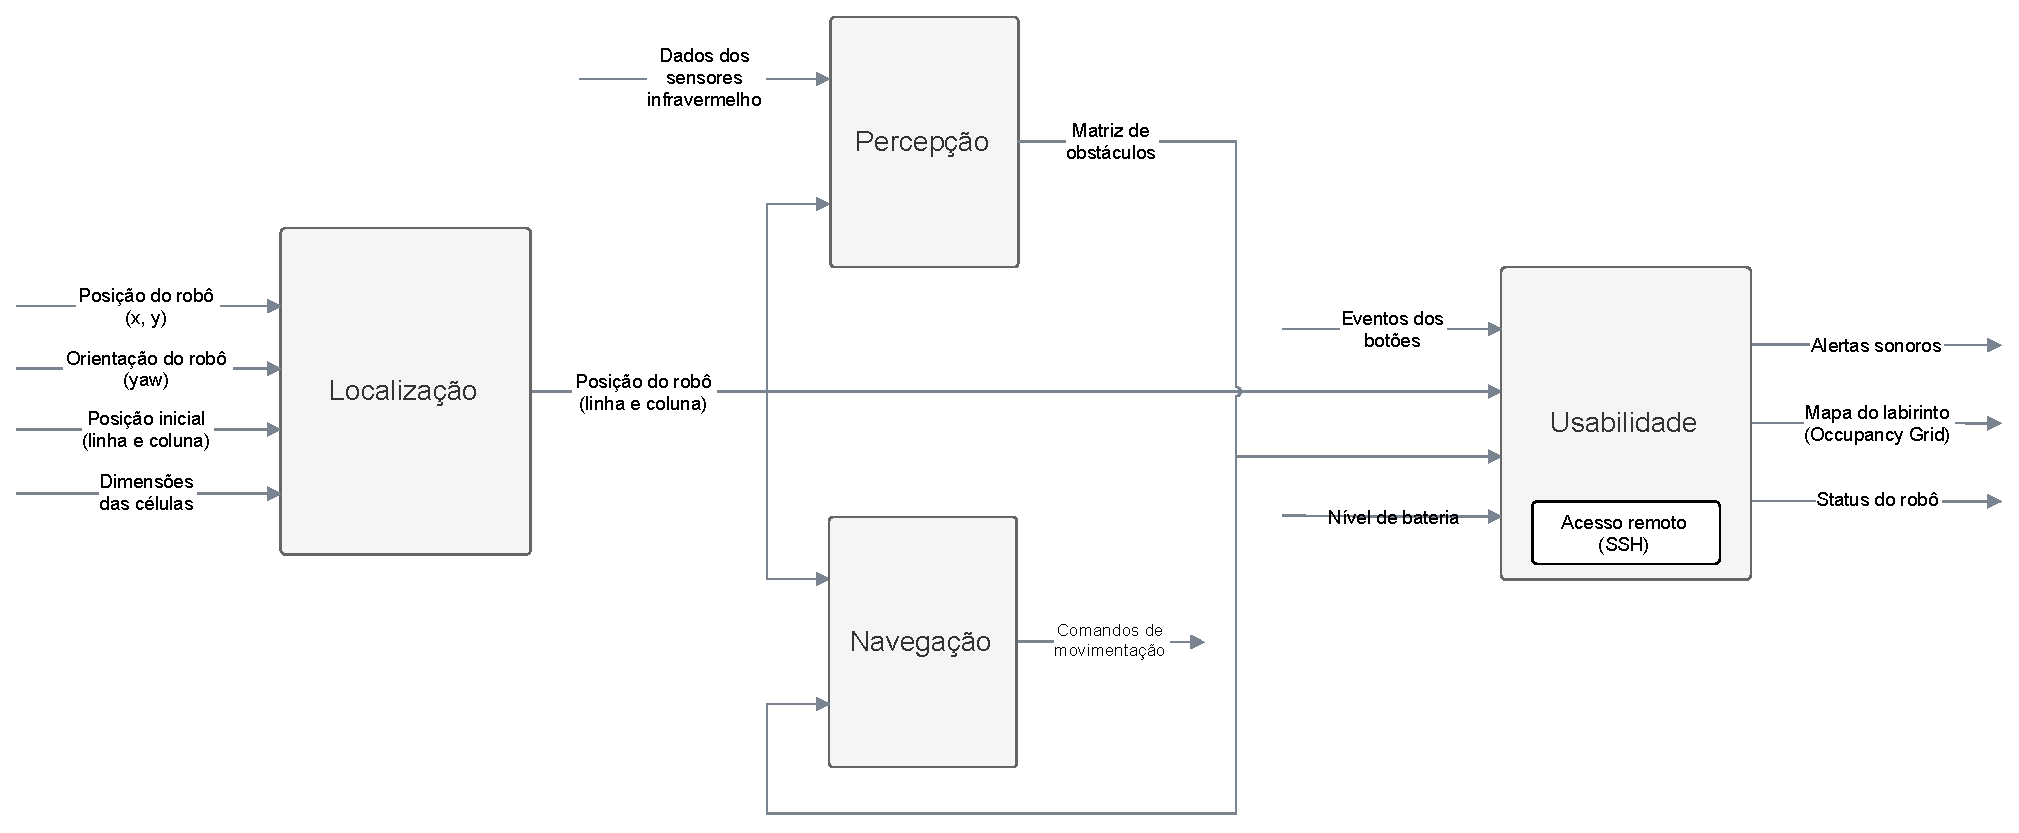
\includegraphics[width=1\textwidth]
	{Figures/especificacao_funcional_geral}
	\label{fig:especificacao_funcional_geral}
	\source{Própria Autoria}
\end{figure}

\subsection{Localização}
\label{ssec:funcionalidade_localizacao}
O labirinto a ser percorrido pelo micromouse será modelado como uma matriz 16 x 16, sendo dividido em células de largura e comprimento fixos. Para que o robô consiga decidir para onde ele deve ir, primeiro é necessário saber onde ele está.

A estratégia utilizada para a obtenção da posição do Doogie utilizará a técnica de Odometria, onde, a partir das informações do Encoder e das dimensões das rodas utilizadas, estima-se a distância percorrida em um intervalo de tempo. Além disso, para melhorar a precisão da medição, será utilizada uma IMU, capaz de fornecer os dados de aceleração e velocidade angular nos três eixos cartesianos.

Uma vez que o robô consiga calcular a distância percorrida, em qualquer intervalo de tempo, sabendo as dimensões de cada célula e assumindo que seu ponto de partida foi informado, é possível determinar as coordenadas do mesmo dentro do labirinto: linha e coluna. 

\subsubsection{Objetivo}
Interpretar as informações fornecidas pela Odometria e identificar a posição do robô dentro do labirinto.

\subsubsection{Dependências}
Esse pacote depende da aquisição de dados publicados por:
\begin{itemize}
	\item Pacote de driver da IMU;
	\item Pacote de driver do motor.
\end{itemize}
	
\subsubsection{Premissas}
Para que essa funcionalidade alcance o seu propósito, assume-se que:
\begin{itemize}
	\item O ponto de partida do robô será informado pelo usuário: [linha, coluna];
	\item O valor de comprimento e largura das células são conhecidos pelo sistema e é diferente de zero;
	\item O valor de comprimento e largura (em metros) das células será previamente informado;
	\item O pacote de \textit{driver} da IMU, aliado ao pacote de \textit{driver} do motor, oferecerão a informação de orientação do robô.
\end{itemize}

\subsubsection{Saídas}
Essa funcionalidade tem como saídas:
\begin{itemize}
	\item Doogie position: localização do robô na matriz, no formato: [linha, coluna].
\end{itemize}

A Figura \ref{fig:especificacao_funcional_localizacao} demonstra as entradas e saídas da funcionalidade em questão.

\begin{figure}[H]
	\centering
	\caption{Fluxograma ilustrativo da funcionalidade de Localização.}
	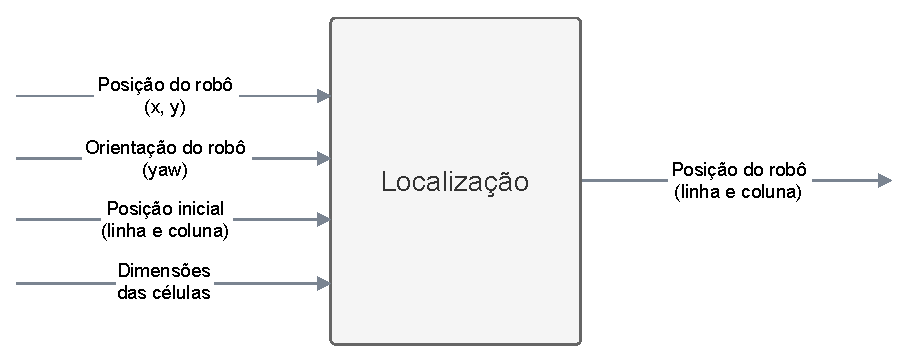
\includegraphics[width=1\textwidth]
	{Figures/especificacao_funcional_localizacao}
	\label{fig:especificacao_funcional_localizacao}
	\source{Própria Autoria}
\end{figure}

\subsection{Percepção}
\label{ssec:funcionalidade_percepcao} 
Para que o \textit{micromouse} consiga se locomover pelo labirinto, é necessário reconhecer os possíveis caminhos, identificando os obstáculos ao seu redor. Utilizando informações obtidas dos sensores infravermelho, essa funcionalidade conseguirá definir a presença de paredes nas proximidades do robô.
 
Como mencionado anteriormente, o labirinto será modelado como uma matriz $mxn$. Será utilizado um sistema de referência absoluto para o mesmo, definindo onde fica o norte, sul, leste e oeste. Com esse sistema de referência, a medida que o robô vai percorrendo o labirinto, em cada célula serão identificadas a presença de paredes. Dessa forma, essa funcionalidade irá publicar uma matriz, contendo a informação da presença de paredes ao norte, sul, leste e oeste de cada célula.

\subsubsection{Objetivo}
Identificar a presença de obstáculos ao norte, sul, leste e oeste de cada célula da matriz que representa o labirinto.

\subsubsection{Dependências}
Esse pacote depende da aquisição de dados publicados por:
\begin{itemize}
	\item Pacote de driver dos sensores infravermelho;
	\item Posição do robô, obtida do pacote de localização. 
\end{itemize}

\subsubsection{Premissas}
Para que essa funcionalidade alcance o seu propósito, assume-se que:
\begin{itemize}
	\item Os sensores infravermelho estarão conectados à Raspberry Pi e a informação dos mesmos está sendo disponibilizada corretamente;
	\item O pacote de localização estará funcionando corretamente, publicando as informações de posicionamento do robô.
\end{itemize}

\subsubsection{Saídas}
Essa funcionalidade tem como saída:
\begin{itemize}
	\item Matriz de dimensão $mxn$ com cada célula contendo valores booleanos para as seguintes variáveis:
	\begin{itemize}
		\item \textit{north}: presença de parede ao norte da célula;
		\item \textit{south}: presença de parede ao sul da célula;
		\item \textit{east}: presença de parede ao leste da célula;
		\item \textit{west}: presença de parede ao oeste da célula.
	\end{itemize}
\end{itemize}

Na Figura \ref{fig:especificacao_funcional_percepcao} pode ser visualizado quais serão as entrada e a saída da funcionalidade Percepção.

\begin{figure}[H]
	\centering
	\caption{Fluxograma ilustrativo da funcionalidade de Percepção.}
	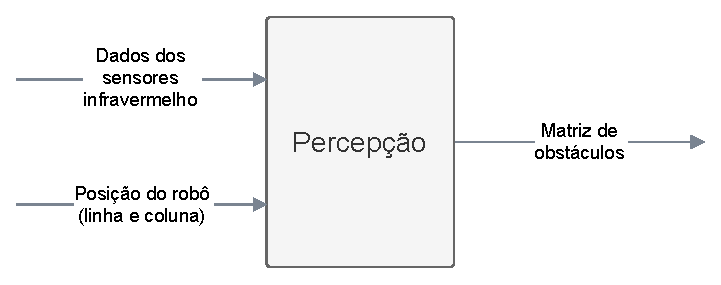
\includegraphics[width=1\textwidth]
	{Figures/especificacao_funcional_percepcao}
	\label{fig:especificacao_funcional_percepcao}
	\source{Própria Autoria}
\end{figure}

\subsection{Navegação}
\label{ssec:funcionalidade_navegacao} 
Para o robô seguir pelo melhor caminho dentro do labirinto é necessário antes que este seja conhecido por ele. Para isso, em um primeiro momento, será necessário que o micromouse percorra o labirinto somente para o seu conhecimento parcial. Então, será necessário a utilização das informações publicadas pelas funcionalidades de Percepção e Localização. Com base nelas, o sistema de navegação poderá definir os comandos necessários para que o robô execute o próximo movimento dentro do labirinto.

O micromouse será programado com 3 estratégias de solução do labirinto diferentes. Essas podem ser selecionadas pelo usuário através da interface de usuário. Primeiramente, o robô irá executar a funcionalidade de mapeamento com base no algoritmo de força bruta, que consiste em sempre que não houver obstáculos a direita, tomar este caminho, movimentando-se de modo diferente somente se for identificado impossibilidade de seguir pela direita. Após isso, o algoritmo de resolução fará com que o robô chegue ao destino final pelo percurso mais otimizado dentro das possibilidades conhecidas previamente pelo mapeamento do labirinto.

\subsubsection{Objetivo}
Planejar trajetórias a fim de garantir a correta locomoção do robô, possibilitando primeiramente o mapeamento do labirinto e após isso a chegada ao destino final pelo caminho mais rápido.

\subsubsection{Dependências}
Esse pacote depende da aquisição de dados publicados por:
\begin{itemize}
	\item Matriz de obstáculos;
	\item Posição do robô: localização do robô na matriz, no formato: [linha, coluna].
\end{itemize}

\subsubsection{Premissas}
Para que essa funcionalidade alcance o seu propósito, assume-se que:
\begin{itemize}
	\item Correto funcionamento dos pacotes de localização e percepção;
	\item Os drivers de potências dos motores estarão conectados à Raspberry Pi e o driver ROS e o sistema de controle dos movimentos do robô estejam funcionando corretamente.
\end{itemize}

\subsubsection{Saída}
Essa funcionalidade tem como saídas:
\begin{itemize}
	\item Comandos de movimentação.
\end{itemize}

As entradas e saída da funcionalidade Navegação podem ser visualizadas na Figura \ref{fig:especificacao_funcional_navegacao}.

\begin{figure}[H]
	\centering
	\caption{Fluxograma ilustrativo da funcionalidade de Navegação.}
	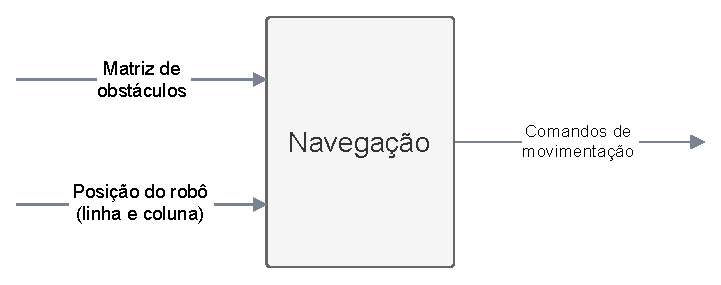
\includegraphics[width=1\textwidth]
	{Figures/especificacao_funcional_navegacao}
	\label{fig:especificacao_funcional_navegacao}
	\source{Própria Autoria}
\end{figure}

\subsection{Usabilidade}
\label{ssec:funcionalidade_usabilidade} 
Para permitir que o usuário interaja com o robô, algumas interfaces são disponibilizadas. A primeira delas consiste do acesso via SSH que perimite o acesso remoto do robô. Usando essa interface é possível acessar a linha de comando do robô para realizar configurações do dispositivo de processamento, compilação de códigos fonte, configuração de parâmetros do robô e execução tanto das rotinas de demonstração do robô quanto das rotinas de resolução de labirintos. Já para que o usuário exerça interação com a plataforma sem a necessidade do acesso remoto, é disponibilizado botões e um buzzer. Esses dois elementos, são utilizados principalmente em competições para facilitar o manuseio do robô.
 
Por fim, quando não utilizado em competições, o mapa do labirinto pode ser visualizado no RViz (visualizador 3D do \textit{framework} ROS) a medida em que ele é percorrido pela plataforma móvel.

\subsubsection{Objetivo}
Permitir que o usuário acesse e edite configurações, execute comandos e monitore o estado do robô.

\subsubsection{Dependências}
Esse pacote depende da aquisição de dados publicados por:
\begin{itemize}
	\item Driver do Buzzer;
	\item Driver dos botões;
	\item Módulo de Localização;
	\item Módulo de Percepção.
\end{itemize}

\subsubsection{Premissas}
Para que essa funcionalidade alcance o seu propósito, assume-se que:
\begin{itemize}
	\item Uma rede comunicação Wireless com a plataforma esteja disponível;
	\item O acesso via SSH seja configurado previamente;
	\item O Buzzer esteja conectado a Raspberry PI e o ROS driver esteja funcionando corretamente;
	\item  Os módulos de Percepção e Localização estejam funcionando corretamente.
\end{itemize}

\subsubsection{Saídas}
Essa funcionalidade tem como saídas:
\begin{itemize}
	\item Alertas sonoros;
	\item Mapa do labirinto (\textit{Occupancy Grid});
	\item Status do robô.
\end{itemize}

As entradas e saída da funcionalidade Navegação podem ser visualizadas na Figura \ref{fig:especificacao_funcional_usabilidade}.

\begin{figure}[H]
	\centering
	\caption{Fluxograma ilustrativo da funcionalidade de Usabilidade.}
	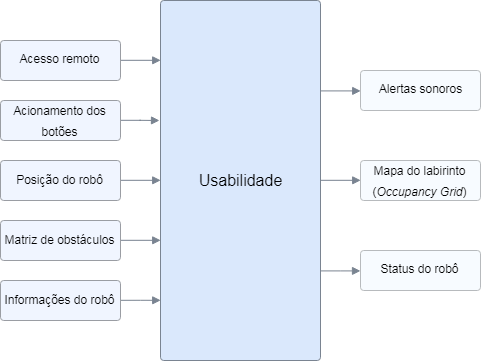
\includegraphics[width=1\textwidth]
	{Figures/especificacao_funcional_usabilidade}
	\label{fig:especificacao_funcional_usabilidade}
	\source{Própria Autoria}
\end{figure}
    \chapter{Resultados}
\label{chap:resultados}
A fase de desenvolvimento do robô Doogie culminou em 3 resultados principais: Protótipo, ambiente de simulação e a estrutura de software da plataforma móvel. Os tópicos posteriores irão detalhar cada um desses resultados. 

%--------- NEW SECTION ----------------------
\section{Protótipo}
\label{sec:resultado_prototipo}
O protótipo é composto por duas placas (placa inferior e placa superior) resultantes da integração de componentes eletrônicos. Na Figura \ref{fig:top_board_elementos}, é possível visualizar alguns dos componentes eletrônicos que compõem a placa superior, quais sejam: a IMU que é responsável por fornecer dados que auxiliam no processo de localização do Doogie dentro do labirinto, os LEDs, Buzzer, Push Buttons que têm por finalidade garantir a interface do usuário com o robô, promovendo indicações luminosas e sonoras. O \textit{Pin Header} da Raspberry que é a conexão física da placa com a própria Raspberry, o Multiplexador Analógico e o Conversor A/D que interagem entre si permitindo a aquisição dos dados dos sensores e da bateria em formato analógico, transformando-os em digital e, por fim, o conversor DC-DC 5V que garante que a tensão de alimentação da Raspberry mantenha-se conforme especificação (5V). Vale ressaltar que o \textit{Pin Header} macho é responsável por permitir a conexão entre as placas inferior e superior.

\begin{figure}[H]
	\centering
	\caption{Componentes da placa superior do Doogie Mouse}
	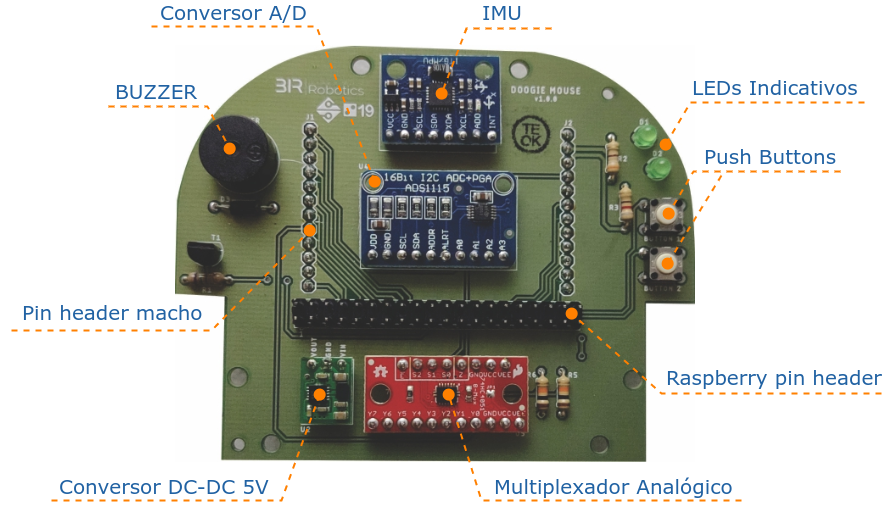
\includegraphics[width=1\textwidth]
	{Figures/top_board_elementos.png}
	\label{fig:top_board_elementos}
	\source{Própria Autoria}
\end{figure}

Sabendo sobre a funcionalidades dos componentes da placa superior, podemos observar agora a figura \ref{fig:bottom_board_elementos}. Os componentes que compõem a placa inferior, cuja parte circulada em cor vermelha refere-se ao conjunto do motor que é formado pelas rodas, \textit{bracket}, micro motor, encoder magnético, \textit{flat cable} e conector IDC fêmea. Esse conjunto é responsável por garantir o correto acionamento e funcionamento do motor, promovendo suas interligações elétricas e mecânicas, fornecendo dados para aprimorar o sistema de controle do motor. É possível identificar 4 pares de sensores infra-vermelho (Emissor IR e Fototransistor) na placa inferior, que são responsáveis por identificar os obstáculos próximos ao robô. Observa-se também o conversor DC-DC 6V que tem função de fornecer para os sensores e motores a tensão necessária para o funcionamento dos mesmos, o componente Ponte H que permite o controle de sentido de giro do eixo dos motores bem com a potência elétrica, as chaves Liga/Desliga que ligam e desligam os circuitos da bateria e dos motores, o conector da bateria que é responsável pela fixação da bateria e o próprio componente bateria que é responsável por fornecer a tensão de alimentação para o funcionamento de ambas as placas. A integração das placas inferior e superior juntamente com a Raspberry é o que compõem o protótipo físico do robô Doogie Mouse (vide Figura \ref{fig:prototipos}).

\begin{figure}[H]
	\centering
	\caption{Componentes da placa inferior do Doogie Mouse}
	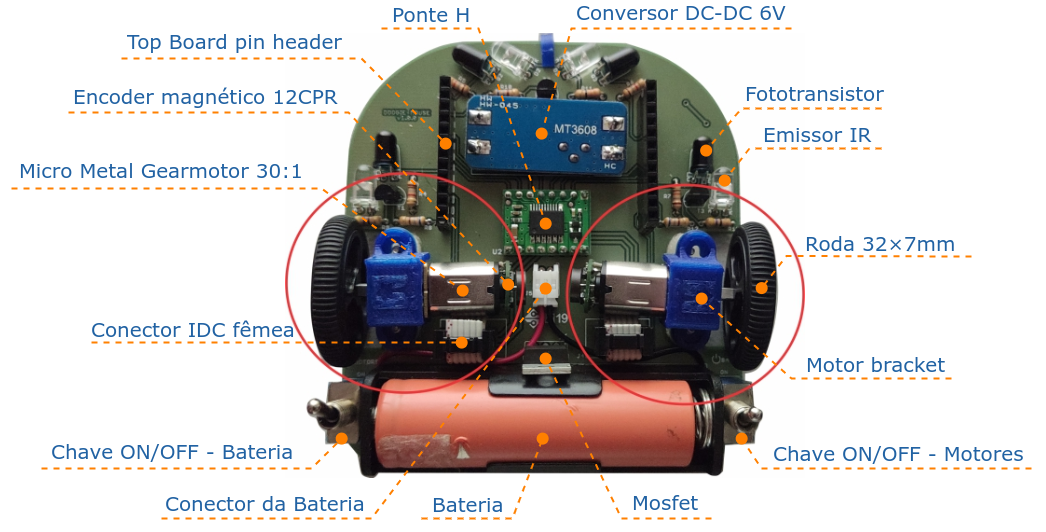
\includegraphics[width=1\textwidth]
	{Figures/bottom_board_elementos.png}
	\label{fig:bottom_board_elementos}
	\source{Própria Autoria}
\end{figure}

\begin{figure}[H]
	\centering
	\caption{Protótipos do Doogie Mouse confeccionados}
	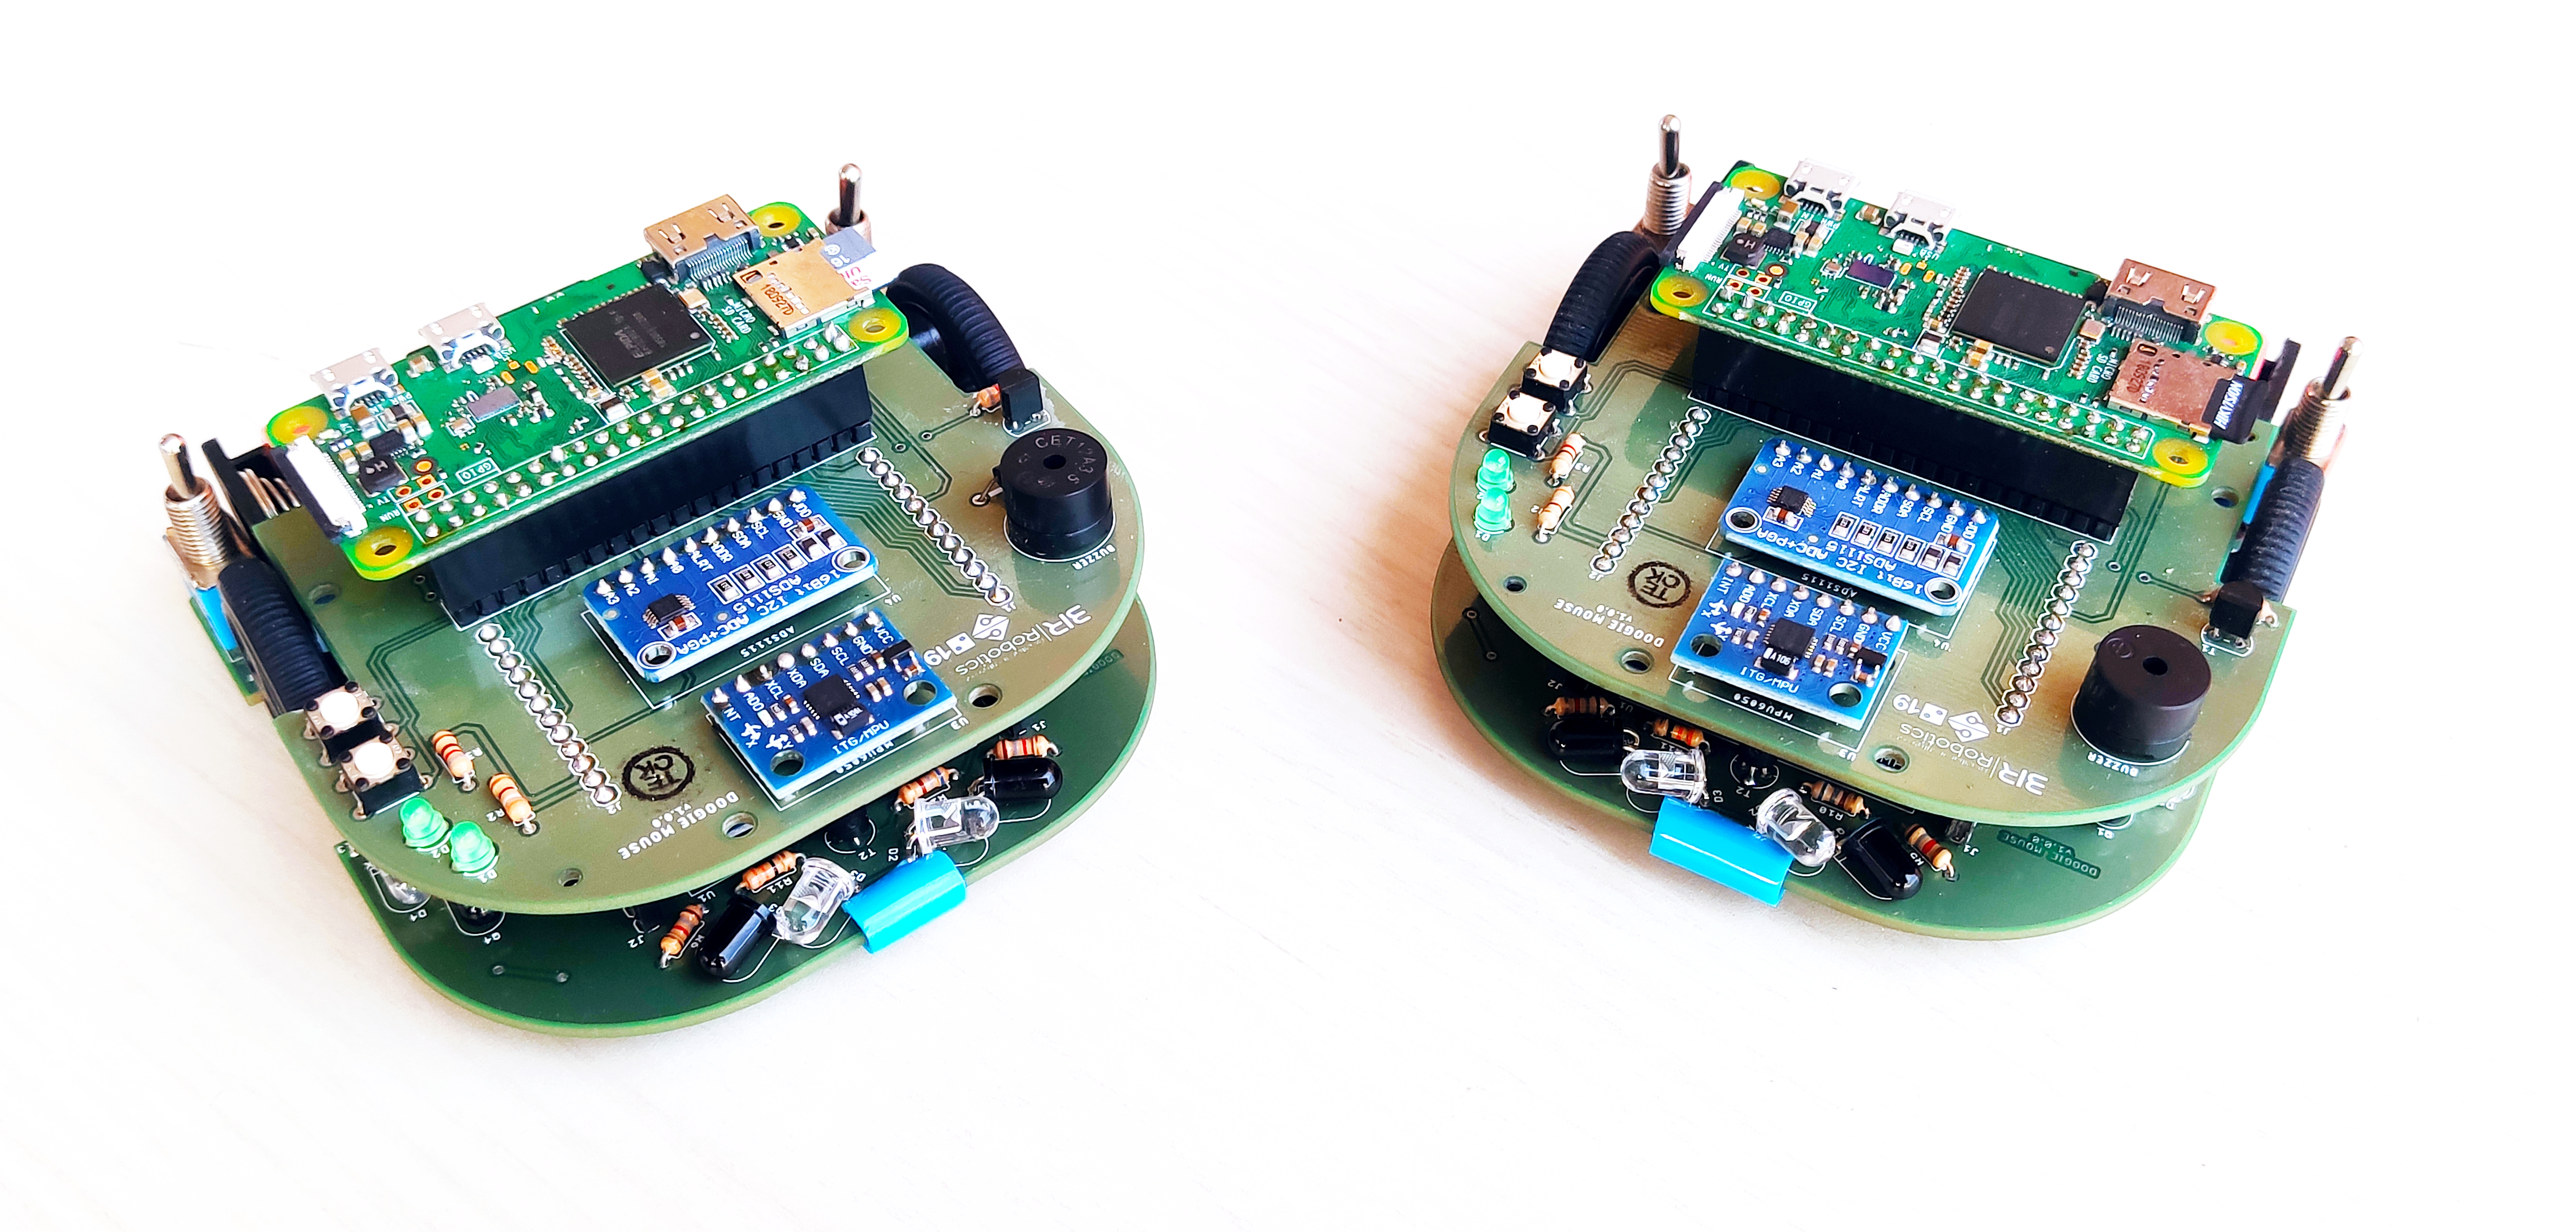
\includegraphics[width=1\textwidth]
	{Figures/doogie_mouse_prototipos}
	\label{fig:prototipos}
	\source{Própria Autoria}
\end{figure}

Visando auxiliar os usuários, o protótipo dispõe de dois guias: um guia de montagem das placas e um guia de configuração de software. O guia de montagem das placas está disponível no site GitHub para acesso por qualquer usuário. Esse guia foi criado para proporcionar ao usuário uma experiência didática com relação à parte de hardware do Doogie e apresenta uma sequência de passos para fixação dos componentes eletrônicos, assim como algumas dicas, que tem por objetivo garantir mais facilidade no decorrer do processo de montagem. Nesse documento também são listados os requisitos físicos necessários para montagem do robô, bem como, ferramentas utilizadas, componentes eletrônicos e os equipamentos de proteção individual (EPI’s), aconselháveis utilização durante todo o procedimento para evitar qualquer tipo de acidente. Com o intuito de eliminar possíveis dúvidas durante as etapas de montagem, o documento supracitado dispõe de imagens que ilustram detalhadamente todo passo a passo de fixação de cada componente. Uma parte desse guia, que possui mais de 34 passos de montagem,  pode ser visualizado na Figura \ref{fig:guia_hardware_setup}. O guia completo pode ser visualizado no Apêndice \ref{apend:doogie_hardware_setup}.

\begin{figure}[H]
	\centering
	\caption{Recorte do guia de instruções de montagem do Doogie Mouse}
	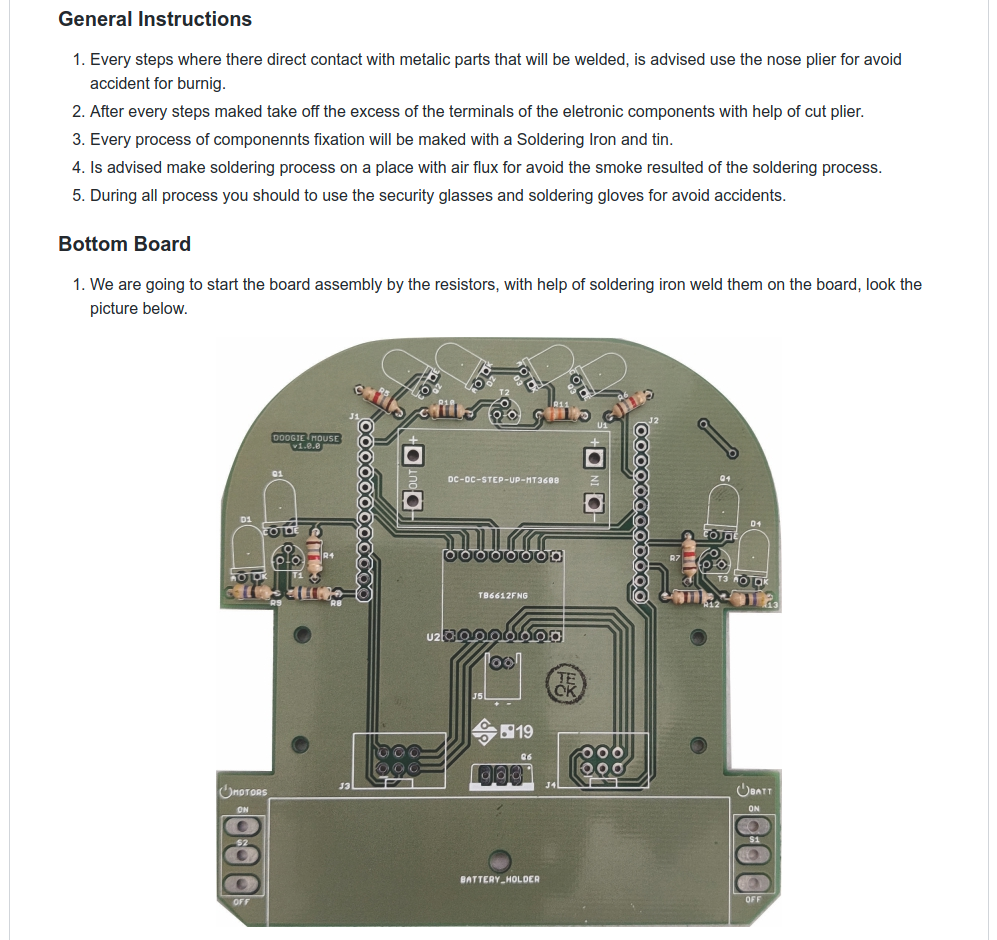
\includegraphics[width=0.9\textwidth]
	{Figures/guia_hardware_setup}
	\label{fig:guia_hardware_setup}
	\source{Própria Autoria}
\end{figure}

De maneira análoga ao guia de montagem das placas, o guia de configuração de software também está disponível no GitHub, conforme ilustrado pela Figura \ref{fig:guia_software_setup}. O manual de configuração de software informa sobre os requisitos físicos necessário para iniciar as configurações e apresenta uma lista com as instruções sobre instalação e resolução de dependência de todos os softwares necessários para o funcionamento do Doogie, que varia desde a preparação da unidade de armazenamento em que é instalado o sistema operacional até um código teste dentro do ambiente do ROS. Esse manual também dispõe de uma galeria de imagens ilustrando as telas de acordo com cada procedimento, garantindo ao usuário um ótimo entendimento das etapas. Este manual pode ser visualizado na íntegra no Apêndice \ref{apend:doogie_software_setup}.

\begin{figure}[H]
	\centering
	\caption{Recorte do guia de instruções de configuração de software do Doogie Mouse}
	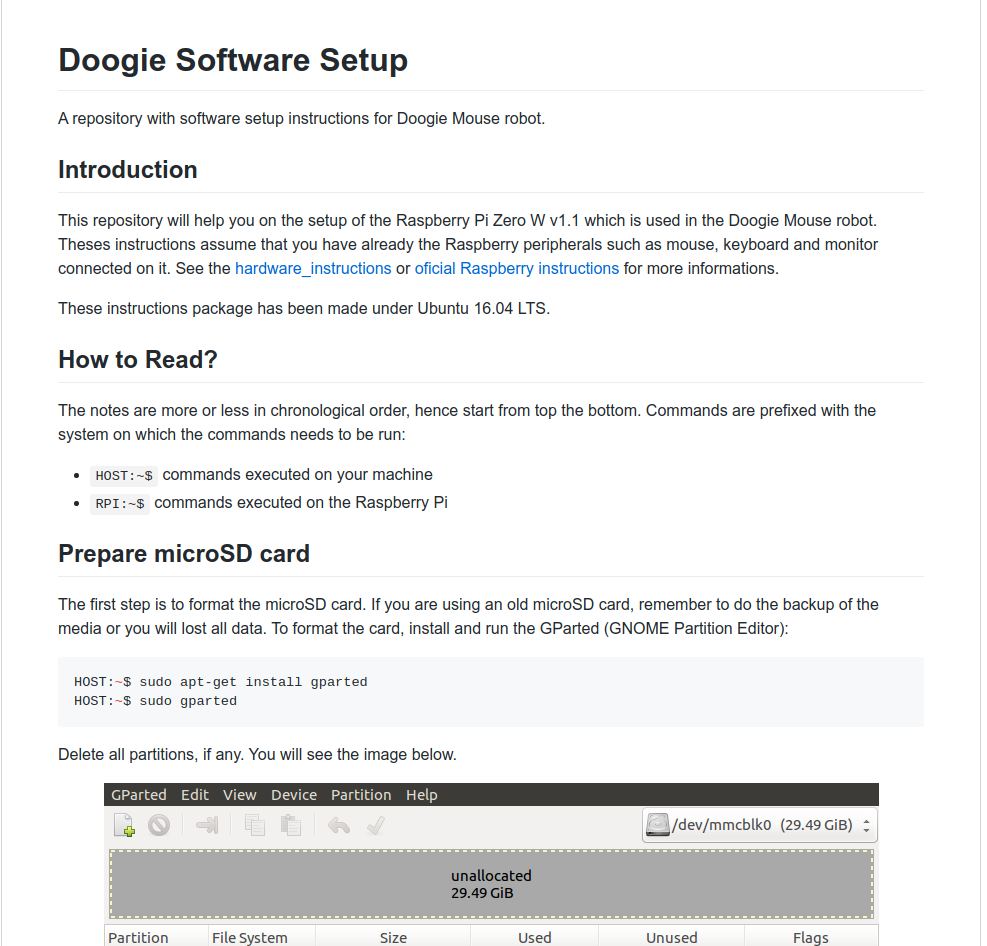
\includegraphics[width=1\textwidth]
	{Figures/guia_software_setup}
	\label{fig:guia_software_setup}
	\source{Própria Autoria}
\end{figure}

\section{Ambiente de simulação}
\label{sec:resultado_ambiente_de_simulacao}
\subsection{Comparativo de Malhas}
\label{ssec:comparativo_de_malhas}
No comparativo de malhas, analisou-se como os formatos \gls{collada} (.dae) e \gls{stl}(.stl) interferem na simulação, bem como o uso de tipos primitivos para a representação da malha de colisão. Na Tabela \ref{tab:ComparativoMalhas}, comparam-se os modelos simplificados, gerado na seção \ref{sec:Simulacao}, usando malhas em \gls*{collada} (Doogie\_lite\_dae) e \gls*{stl} (Doogie\_lite\_stl), e o modelo 3D sem simplificações (Doogie\_real\_dae) gerado na seção \ref{sec:modelo_mecanico} usando sua malha em \gls*{collada}.

\begin{table}[H]
	\centering
	\caption{Comparativo entre malhas carregadas no Gazebo}
	\begin{tabular}{|l|l|l|l|l|}
		\hline
		& \multicolumn{1}{c|}{\textbf{\begin{tabular}[c]{@{}c@{}}Visual\\ (Faces)\end{tabular}}} & \multicolumn{1}{c|}{\textbf{\begin{tabular}[c]{@{}c@{}}Colisão\\ (Faces)\end{tabular}}} & \multicolumn{1}{c|}{\textbf{FPS}} & \multicolumn{1}{c|}{\textbf{\begin{tabular}[c]{@{}c@{}}Real Time \\ Factor\end{tabular}}} \\ \hline
		\textbf{Doogie\_lite\_dae} & 70.410                                                                                 & 70.410                                                                                  & $\sim$1,5                         & 0,35                                                                                      \\ \hline
		\textbf{Doogie\_real\_dae} & 1.091.337                                                                              & 1.091.337                                                                               & $\sim$0,6                         & 0,03                                                                                      \\ \hline
		\textbf{Doogie\_lite\_stl} & 70.398                                                                                 & 70.398                                                                                  & $\sim$4.2                         & 0,33                                                                                      \\ \hline
	\end{tabular}
	\label{tab:ComparativoMalhas}
	\source{Própria Autoria}
\end{table}

O formato \*gls{collada} possui perfomance na simulação ligeiramente inferior ao \gls*{stl}, principalmente em relação ao \gls*{fps} no qual foi 36\% inferior ao desempenho da outra malha. Também fica visível a necessidade da simplificação do modelo do robô, sendo inviável a simulação do Doogie\_real\_dae que teve seu \gls*{fps} inferior a um e o \gls*{rtf} próximo a zero, denotando uma simulação lenta e de pouca acurácia. 


\begin{table}[H]
	\centering
	\caption{Comparativo com simplificação da malha de colisão}
	\begin{tabular}{|l|l|l|l|l|}
		\hline
		& \multicolumn{1}{c|}{\textbf{\begin{tabular}[c]{@{}c@{}}Visual\\ (Faces)\end{tabular}}} & \multicolumn{1}{c|}{\textbf{\begin{tabular}[c]{@{}c@{}}Colisão\\ (Faces)\end{tabular}}} & \multicolumn{1}{c|}{\textbf{FPS}} & \multicolumn{1}{c|}{\textbf{\begin{tabular}[c]{@{}c@{}}Real Time \\ Factor\end{tabular}}} \\ \hline
		\textbf{Doogie\_lite\_dae} & 70.410                                                                                 & 6                                                                                       & $\sim$8,0                         & 0,52                                                                                      \\ \hline
		\textbf{Doogie\_real\_dae} & 1.091.337                                                                              & 6                                                                                       & $\sim$3,5                         & 0,52                                                                                      \\ \hline
	\end{tabular}
	\label{tab:ComparativoMalhaSimplificada}
	\source{Própria Autoria}
\end{table}

Ao comparar o desempenho como uso do modelo simplificado e o modelo real, usando tipos primitivos para a representação da malha de colisão pode-se perceber que o gargalo da simulação se encontra no número das faces de colisão usadas para a representação dinâmica do robô. A taxa de \gls*{fps} aumentou em seis vezes em relação a análise anterior, atingindo um \gls*{rtf} igual ao do modelo simplificado, conforme visto na Tabela \ref{tab:ComparativoMalhaSimplificada}. Sendo assim a configuração Doogie\_lite\_dae com a simplificação da malha de colisão a mais otimizada para uso na simulação sem perda de cor e textura do modelo do robô.


\subsection{Modelos da Simulação}
\label{sec:modelos_sim}
\begin{figure}[H]
	\centering
	\caption{Doogie Mouse no Gazebo}
	\subfigure[Juntas do robô]{\label{fig:doogie_gazebo_joints}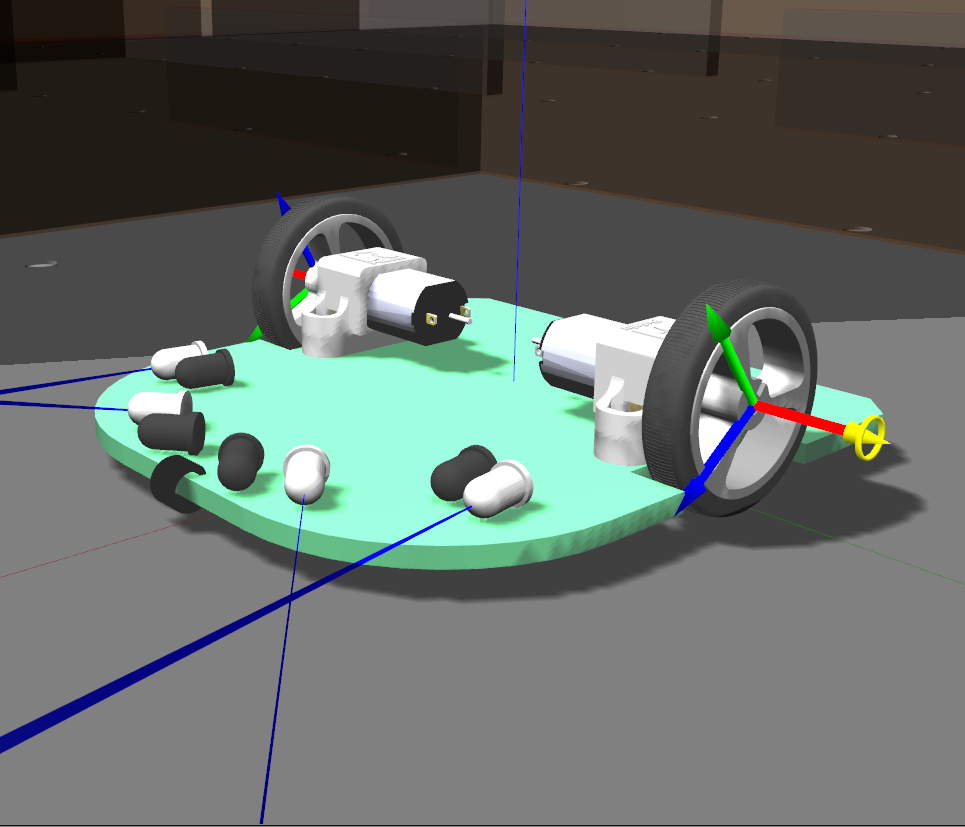
\includegraphics[scale=0.198]{doogie_gazebo_joints}}
	\subfigure[Visualização das transformadas e centro de gravidade]{\label{fig:doogie_gazebo_tfs}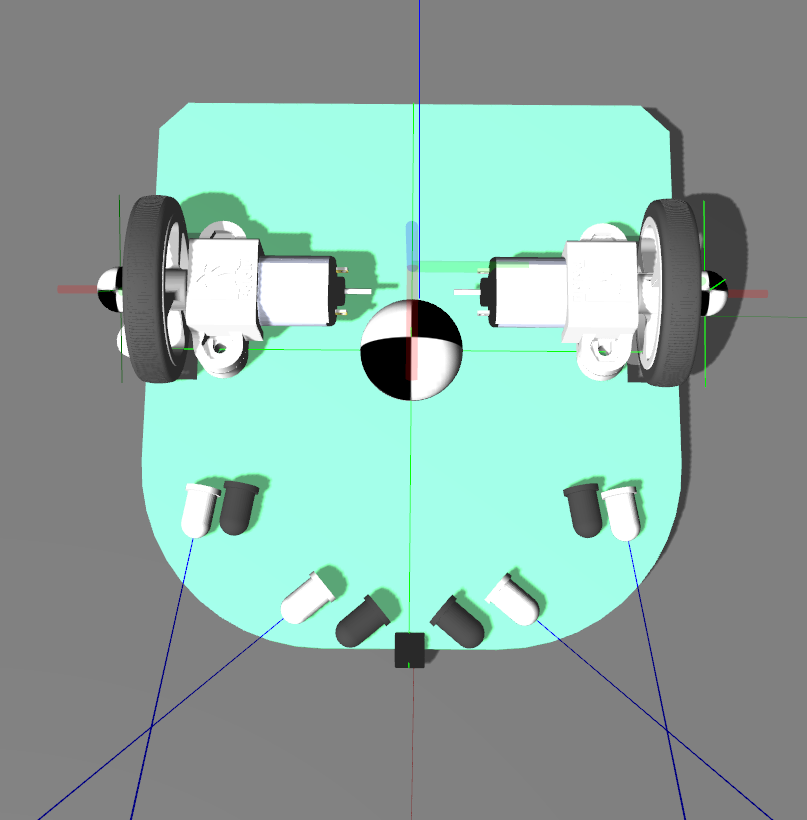
\includegraphics[scale=0.2]{doogie_gazebo_tfs}}
	\subfigure[Modelo renderizado no Gazebo]{\label{fig:doogie_gazebo}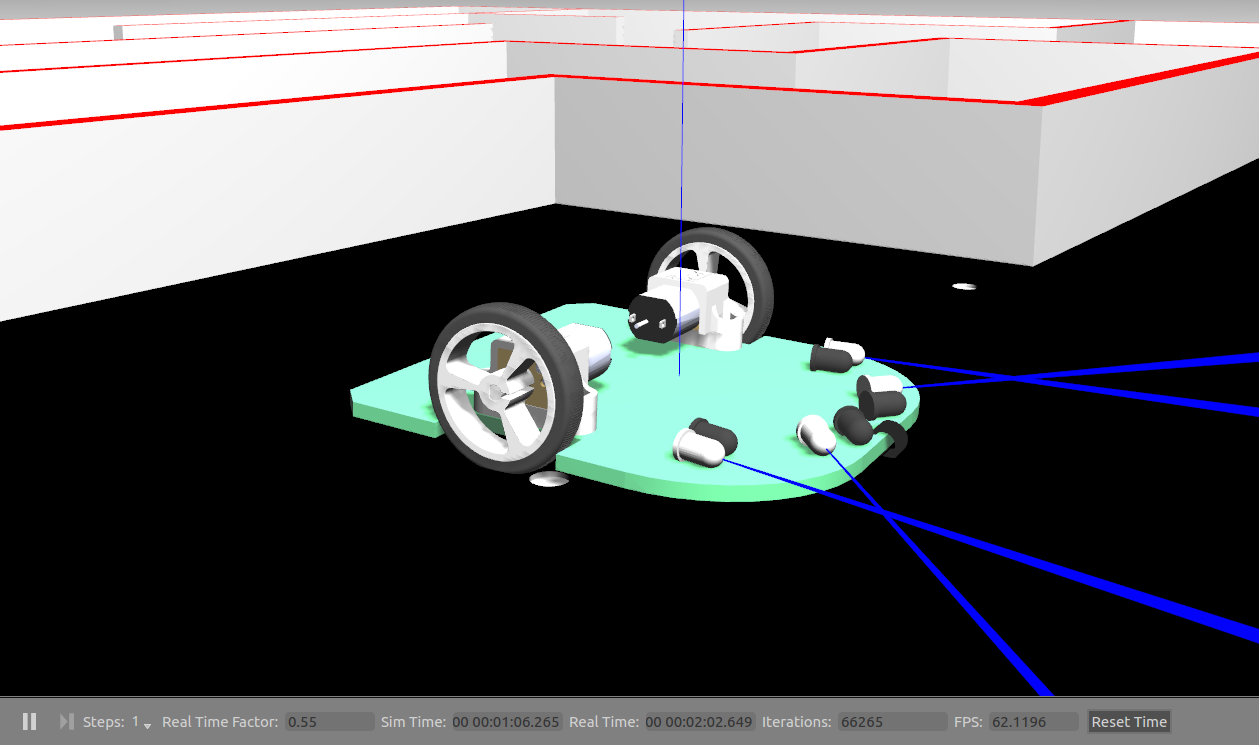
\includegraphics[scale=0.38]{doogie_gazebo}}
	\label{fig:doogie_gazebo_imgs}
\end{figure}
Os modelos exportados para o Gazebo, seguindo a metodologia descrita na seção \ref{sec:Simulacao}, simplificando o modelo 3D gerado pelo SolidWorks, e usando a configuração otimizada obtida no comparativo de malhas da subseção \ref{ssec:comparativo_de_malhas}, do robô e do labirinto foram elaborados de forma a não comprometer a simulação em sua acurácia de ser realizada próxima do tempo real, \gls*{rtf}, ou na sua taxa de atualização de quadros \gls*{fps}. Assim, atingiu-se a simulação simultânea de ambos os modelos, sem comprometimento desses indicadores e em máquinas mais recentes a simulação pode chegar a se manter dentro de 60 \gls*{fps}, a taxa mais comum de de atualização usada nos monitores comerciais.

Dessa forma, provê-se um ambiente de simulação que facilite o acesso dos usuários ao Doogie Mouse, mesmo que para esses não seja possível adquirir a plataforma física, tornando-o mais acessível em sua proposta de ensino.



\label{sec:modelos_sim}
\begin{figure}[H]
	\centering
	\caption{Labirinto na Simulação}
	\subfigure[Labirinto renderizado no Gazebo]{\label{fig:maze_gazebo}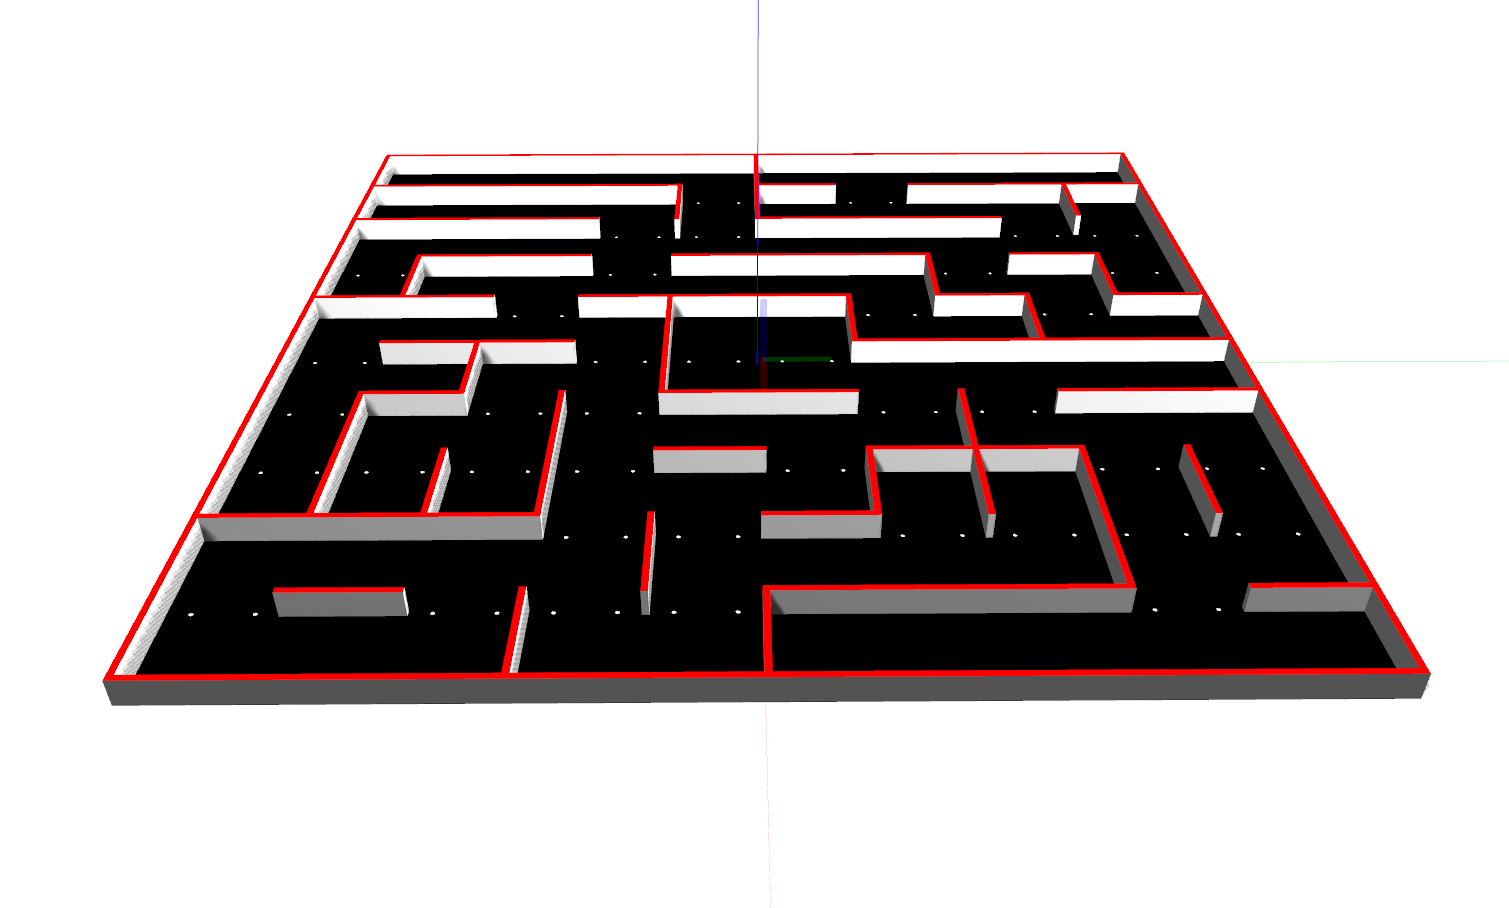
\includegraphics[scale=0.198]{maze_gazebo}}
	\subfigure[Malha de colisão das paredes]{\label{fig:minus_gazebo_colisions}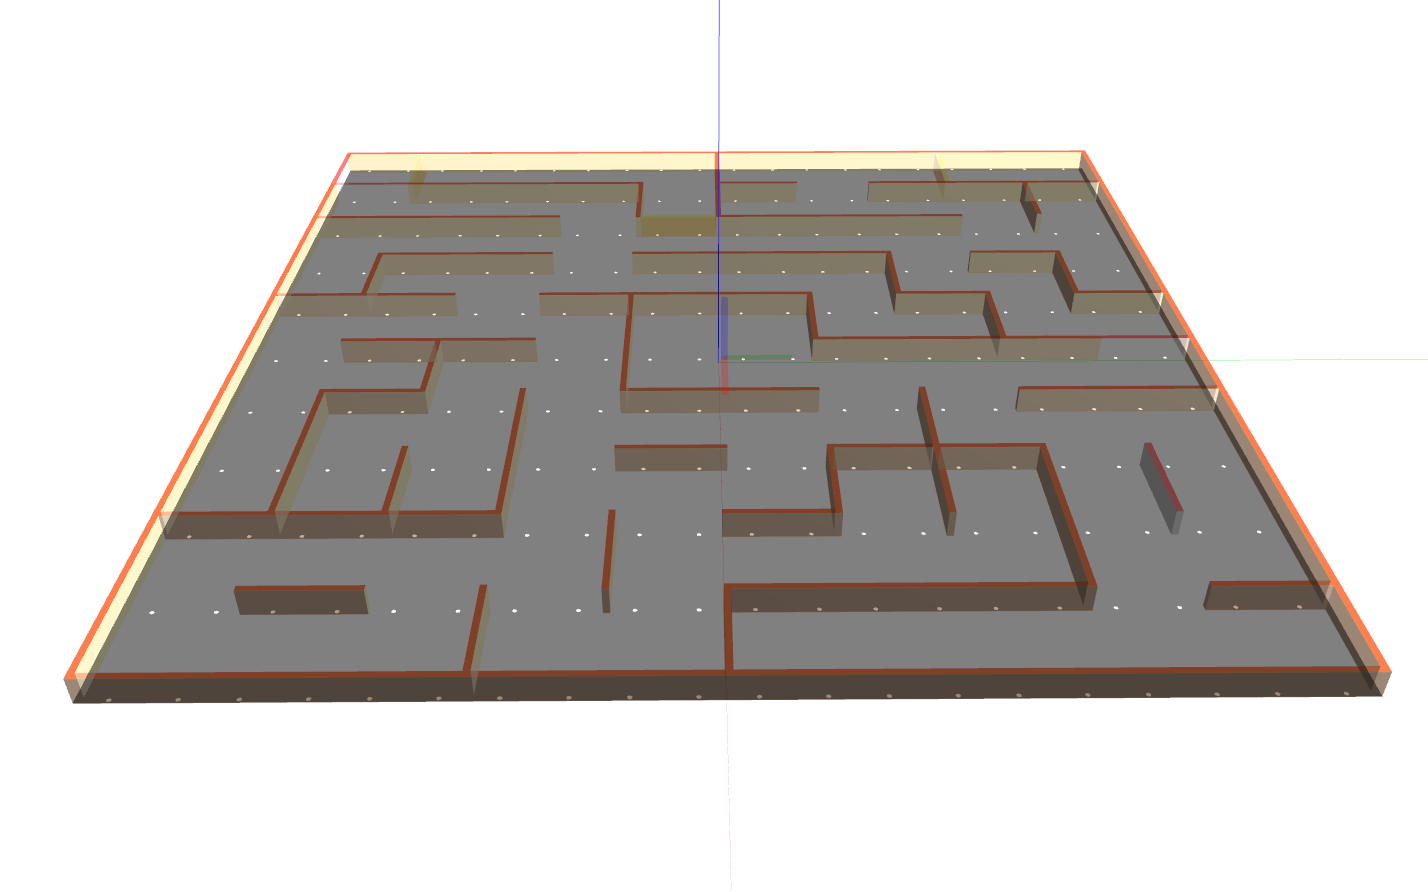
\includegraphics[scale=0.25]{minus_gazebo_colisions}}
	\label{fig:minus_gazebo_imgs}
\end{figure}

%--------- NEW SECTION ----------------------
\section{Estrutura de Software}
\label{sec:resultado_estrutura_de_software}
Para contemplar o objetivo do projeto, que é ser uma plataforma para aprendizagem de robótica móvel e inteligência artificial, optou-se pelo uso do \textit{framework} \gls*{ros} devido a sua capacidade de abstração de hardware e de reuso de software como já mencionado em \ref{sec:robotic_frameworks}. Diante disso, foi criada uma estrutura de software modular que pode ser visualizada na Figura \ref{fig:doogie_packages}. Essa estrutura é formada por \textit{stacks}, que são conjunto de pacotes agrupados em um mesmo local. Abaixo está descrito qual o objetivo de cada pacote dentro dessas \textit{stacks}.

\textbf{doogie\_base}:
\begin{itemize}
	\item \textbf{doogie\_algorithms}: Contém os algoritmos de inteligência que são utilizados pelo robô na resolução do labirinto;
	\item \textbf{doogie\_control}: Possui arquivos de configuração e de inicialização dos processos de controle do robô;
	\item \textbf{doogie\_description}: Abarca arquivos com a descrição do modelo do robô;
	\item \textbf{doogie\_msgs}: Compreende as estrutura de dados (.msg e .action) criadas exclusivamente para o Doogie Mouse;
	\item \textbf{doogie\_navigation}: Abrange os processos utilizados para a percepção, localização e navegação do robô dentro do labirinto. Fornece também \glspl*{api} para permitir que usuários implementem sua própria estratégia de resolução de labirinto.   
\end{itemize}
	
\textbf{doogie\_simulator}:
\begin{itemize}
	\item \textbf{doogie\_gazebo}: Integra todos os arquivos de configuração necessários para executar o ambiente de simulação.
\end{itemize}
	
\textbf{doogie\_robot}
\begin{itemize}
	\item \textbf{doogie\_bringup}: Agrupa arquivos de configuração e inicialização de todos os subsistemas do robô. Contém também os executáveis responsáveis pela atuação da plataforma móvel.  
	\item \textbf{doogie\_drivers}: Compreende executáveis e bibliotecas dos componentes de hardware do robô (motor, Encoder, \gls*{imu} e sensores infravermelho).
\end{itemize}
	
\textbf{doogie\_desktop}
\begin{itemize}
	\item \textbf{doogie\_rviz}: Engloba arquivos de configuração e inicialização para visualização de dados do robô no visualizador RViz;
	\item \textbf{doogie\_welcome}: Contém executáveis para verificação do funcionamento do \textit{framework} ROS na etapa de instalação.
\end{itemize}

\begin{figure}[H]
	\centering
	\caption{Organização dos pacotes do Doogie Mouse.}
	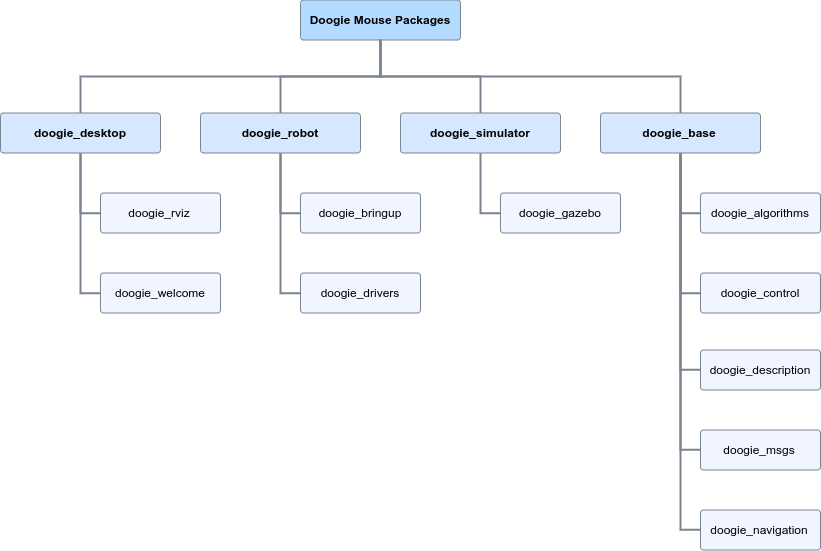
\includegraphics[width=1\textwidth]
	{Figures/doogie_packages}
	\label{fig:doogie_packages}
	\source{Própria Autoria}
\end{figure}

Dentre as \textit{stacks} e pacotes listados na Figura \ref{fig:doogie_packages} apenas a \textit{stack} doogie\_desktop e o pacote doogie\_rviz não foram criados. Os demais estão disponíveis para utilização no repositório remoto GitHub.

Embora todos esses pacotes tenham sido criados, nem todos eles são empregados no funcionamento da plataforma móvel. Como alguns pacotes são utilizados apenas para simulação do robô, não há a necessidade da sua utilização dentro da plataforma. Dessa forma, os pacotes foram organizados de acordo com o propósito final: utilização no ambiente de simulação, no robô físico ou em ambos. A Figura \ref{fig:diagrama_dos_pacotes} demonstra como esses pacotes se relacionam entre si. A \textit{stack} doogie\_base é comum tanto ao ambiente de simulação quanto ao robô físico, porém, não tem utilidade se não utilizada dentro desses dois contextos. A \textit{stack} doogie\_robot possui todos os pacotes essenciais para o funcionamento do robô físico, entretanto, possui dependência direta com a \textit{stack} doogie\_base. Em oposição está a \textit{stack} doogie\_simulator válida apenas para uso do ambiente de simulação, mas igualmente a doogie\_robot, depende da doogie\_base para funcionar. Englobando todas as \textit{stacks} mencionadas bem como a reunião de toda a documentação do robô está a \textit{stack} doogie\_desktop. A relação de dependência entre esses pacotes é feita através de arquivos de configuração que são utilizados no processo de compilação dos pacotes através de ferramentas específicas do \textit{framework} ROS. Caso uma dependência não seja satisfeita, por exemplo uma \textit{stack} não instalada, um erro ocorrerá.   

\begin{figure}[H]
	\centering
	\caption{Relação de dependência das \textit{stacks} do Doogie Mouse.}
	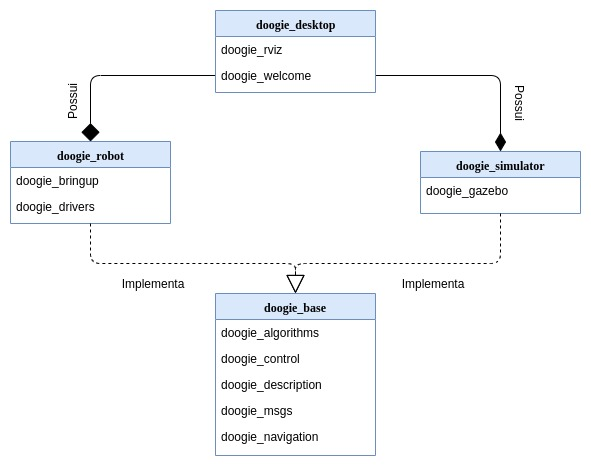
\includegraphics[width=1\textwidth]
	{Figures/diagrama_dos_pacotes}
	\label{fig:diagrama_dos_pacotes}
	\source{Própria Autoria}
\end{figure}

Continuando com a proposta de modularidade de sistemas para proporcionar um grau de flexibilidade no uso de diferentes estratégias de resolução do labirinto, foi pensado, embora não testado, um modelo de comunicação entre os processos dentro do ambiente \gls*{ros}, conforme ilustrado pela Figura \ref{fig:doogie_ros_graph}.

\begin{figure}[H]
	\centering
	\caption{Diagrama de comunicação entre processos.}
	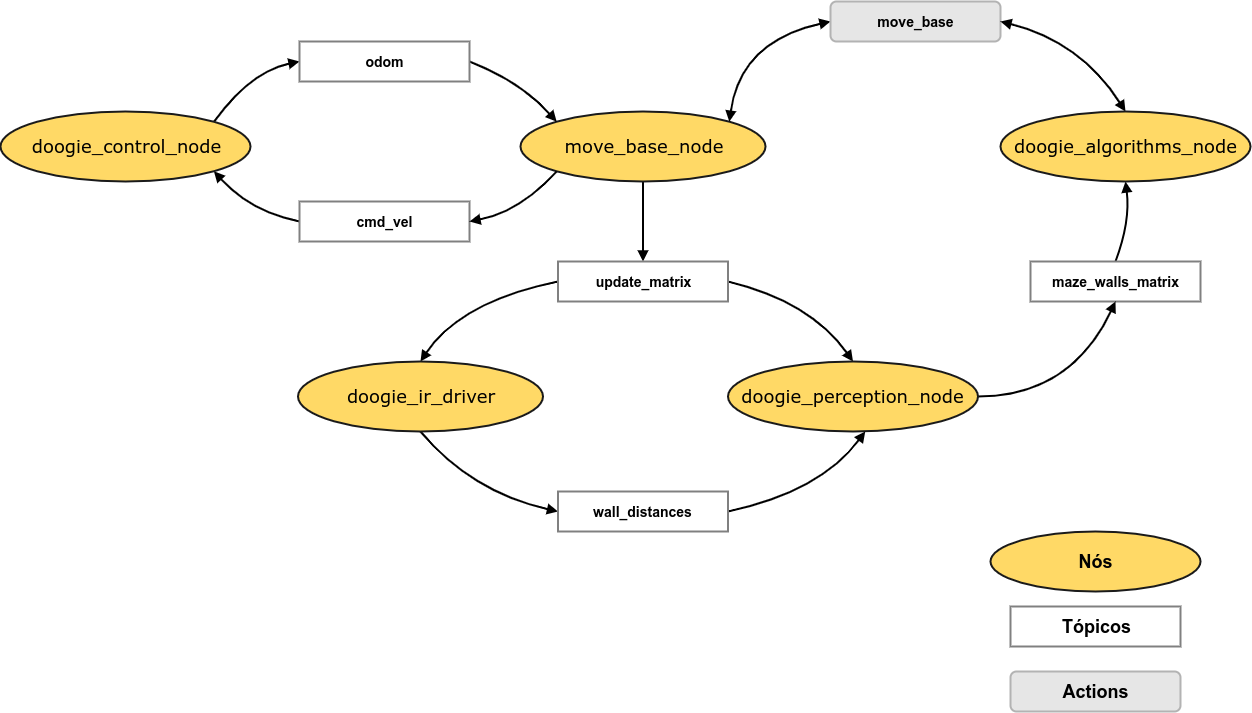
\includegraphics[width=1\textwidth]
	{Figures/doogie_ros_graph}
	\label{fig:doogie_ros_graph}
	\source{Própria Autoria}
\end{figure}

Partindo da premissa que a posição e orientação inicial da base móvel dentro do labirinto é conhecida, a movimentação do robô começa com o doogie\_algorithms\_node enviando um comando de movimentação para o move\_base\_node. Após interpretado qual movimento a plataforma deve executar, o processo move\_base\_node enviará valores de velocidade linear e angular através do tópico cmd\_vel para o processo responsável pelo controle de movimentação do robô. Com o \textit{feedback} de Odometria, o move\_base\_node infere se o robô chegou ao destino desejado. Enquanto o robô está se movimentando, uma informação de progresso é enviada para o doogie\_algorithms\_node de modo que ações possam ser tomadas enquanto o robô se locomove, como emitir uma alerta sonoro quando 90\% do trajeto for concluído																																																																																																																																																																																																																																																																																					.Quando o robô chega ao seu destino final (uma determinada célula do labirinto), uma informação de posição e orientação do robô é fornecida através do tópico update\_matrix. Essa informação é armazenada pelo processo de percepção e dispara também uma requisição para que os dados dos sensores infravermelhos sejam fornecidos. Após a requisição de dados, o \textit{driver} dos sensores infravermelho irá providenciar no tópico wall\_distances as informações de distância das paredes do labirinto. Com os valores de distância, posição e orientação do robô, o processo doogie\_perception\_node sintetiza uma matriz de obstáculos fornecendo em relação a um referencial global quais paredes existem para cada célula do labirinto visitada. Essa matriz é então fornecida para o processo que contém a estratégia de resolução do labirinto escolher a próxima ação de movimentação do robô. Essas etapas se repetem até que o robô encontre o centro do labirinto.

Com essa proposta de organização de comunicação entre processos e de posse das \glspl*{api} fornecidas para envio de comandos de movimentação do robô e manuseio da matriz de obstáculos, o usuário pode implementar sua própria estratégia de resolução de labirinto. O fator limitante de qual abordagem dentro da IA utilizar será apenas o poder de processamento da Raspberry Pi.
    %\chapter{Título do capítulo}\label{chapter:outro}

As organizações atuam em um ambiente global altamente competitivo, dinâmico, complexo e instável. Tais características denotam cenários de imprevisibilidade, onde todas as suas operações e atividades precisam ser vistas e revistas continuamente. Neste contexto do mundo dos negócios, é de fundamental importância que as organizações busquem estratégias eficazes para suas operações - planejamento, marketing, finanças, produção, qualidade e a logística - por serem cada vez mais importantes e por estarem relacionadas diretamente com as atividades fim dos variados sistemas produtivos.

Busca-se, portanto, reduzir custos em toda cadeia de valor e prover a satisfação dos clientes. Por esta ótica é possível entender o porquê da logística está em evidência na conjuntura atual de mercado. O fato desta ser amparada nos pilares: transportes, gestão de estoques, processamento de pedidos, atividades de apoio e ter como objetivo prover o cliente com os níveis de satisfação desejados pelos mesmos, faz com que a logística assuma um papel fundamental para as organizações: ser um componente capaz de gerar uma vantagem competitiva fundamental, ou seja, providenciar bens e serviços de maneira correta, em tempos e lugares exatos, na condição desejada e em menor custo possível.

Entretanto, quando se fala em melhoria da eficiência operacional na distribuição física, não é suficiente considerar apenas o meio de transporte mais utilizado no Brasil - o rodoviário; é preciso, analisar toda matriz de transporte disponível, para alcançar um serviço capaz de atender satisfatoriamente o canal de vendas. Essa visão considera cada etapa do processo de transporte, procurando sempre identificar as possíveis alternativas, muitas vezes descartadas ou mal exploradas.

Conforme Lambert, Stock e Vantine (1998), estima-se que no Brasil os gastos com atividades logísticas correspondam a 17\% do Produto Interno Bruto (PIB) e, na média, o transporte envolve 60\% dos custos logísticos das empresas. Estes dados justificam a necessidade de um sistema de transporte possuir mecanismos capazes de analisar quais opções de modais apresentam-se mais adequadas ao seu contexto de negócio. Ressalta-se ainda, que a seleção de modais afeta diretamente o preço dos produtos, as condições de entrega e a pontualidade, elementos estes considerados estratégicos para que o sistema alcance seu objetivo.

Segundo os mesmo autores, os cinco principais modais básicos são: rodoviário, ferroviário, aquaviário, dutoviário e aéreo, e sua importância relativa deve ser medida em termos de quilometragem do sistema, volume de tráfego, receita e natureza de composição. Justamente por tais questões que o modal aquaviário se configura como uma alternativa importante para a matriz de transportes brasileira, principalmente quando se fala em cabotagem, devido as características geográficas do Brasil.

Qualquer pesquisa efetuada no Brasil sobre modal aquaviário depara-se imediatamente com a seguinte questão fundamental: por que esse modal logístico é menos usado do que a lógica indicaria? O mesmo é verdade para o modal ferroviário. Por que são tão minguados face ao modal rodoviário? Qual a causa desse "transtorno dos modais", essa terrível modalidade de doença logística que aflige o Brasil e constitui uma de suas mais graves patologias?

Muitos estudos têm analisado essa síndrome de hipertrofia rodoviária e anemias ferroviária e aquaviária. Segundo a COPPEAD-UFRJ, o modal rodoviário responde por cerca de 60% de tudo que é transportado no país, enquanto em países de dimensões territoriais equivalentes ao Brasil, como os EUA e a Rússia, esses percentuais são, respectivamente, 35% e 19%.

Independentemente de comparações entre países, salta aos olhos imediatamente o absurdo de se transportar por caminhão cargas de São Paulo a Fortaleza ou Belém, em trajetos de mais de 3.000 km, quando existe a possibilidade de se usar a cabotagem, mais econômica e menos poluidora.

A considerável literatura técnica que versa sobre cabotagem refere-se quase exclusivamente à carga geral conteinerizada, porque é nessa área que reside o maior potencial de alteração de modal. Em matéria de granéis líquidos e sólidos, a maior parte do que pode ser transportado por cabotagem já o está sendo. Ademais, nesse caso, o transporte dutoviário é geralmente mais indicado.

As lamentações sobre a pouca utilização do modal de cabotagem devem ser entendidas como referentes sobretudo à submodalidade de carga geral. Mas há também absurdas quantidades de caminhões transportando granéis sólidos e líquidos a grandes distâncias nas estradas nacionais. A cabotagem, por sua vez, é parte de uma categoria mais ampla, o modal aquaviário ou hidroviário, dividido em dois submodais: cabotagem e transporte fluvial, esse chamado também de navegação interior, que envolve rios, canais e lagoas.

Portanto, pode-se afirmar que o processo de globalização, o transporte intermodal e as revoluções tecnológicas dos últimos anos na indústria de transporte fluvial resultaram em uma busca maior pela otimização das operações de empresas diretamente envolvidas nesse modal e, principalmente, na expansão das chamadas redes marítimas. No entanto, a falta de dados precisos sobre as relações entre os portos, vem impedindo uma maior aplicação da teoria de redes marítimas, que muitas vezes são analisadas por meio de estudos de caso de empresas ou regiões específicas.

A pesquisa e análise do referencial teórico especializado, na área de redes marítimas, demonstram que a grande maioria dos estudos e produção científica investigam pouco a resolução de problemas específicos sobre essas redes, especialmente observando importantes fatores diretamente relacionados a elas como movimentação de cargas, que interferem de maneira coordenada e agregadora no comportamento individual de cada nó dessa rede, ou seja, os portos.

Assim sendo, as análises de redes marítimas se constituem como um dos maiores campos a serem explorados pela evolução do conceito de redes sociais. Neste sentido, este projeto objetiva analisar a estrutura espacial e dinâmica regional da movimentação de contêineres por cabotagem entre os principais portos na costa brasileira, contribuindo com o estado da arte da seguinte maneira: (1) construindo e analisando redes marítimas, com a utilização de softwares especializados para modelagem computacional dessas; (2) hierarquizando os portos brasileiros através da metodologia AHP e (3) identificando possíveis formações de "clusters" entre os operadores logísticos envolvidos nessas redes através das chamadas constelações competitivas. O resultado da junção dessas análises poderá potencializar positivamente a cabotagem brasileira na obtenção de importantes impactos relacionados à sua gestão.

    %
\chapter{Scenario Definitions and Network Analysis}\label{chpdata}

This chapter illustrates the use of our model to represent a real world population,
summarises the model's options and examines the properties of the underlying small world
network representation for a variety of scenarios. It highlights and contrasts the
model's strengths and weaknesses as compared with the original small world model
\cite{Watts1998} and traditionally used social network models.


\section{Scenarios}

The data used to define the population scenarios for analysis and validation of this
model comes from Brazil. A national study conducted in 2000, evaluated the sexual
behaviour of the Brazilian population and perception of HIV/AIDS \cite{msbrasil2000}. The
study consisted of a face to face interview of 3,600 males and females ageing between 16
and 65 years and living in urban areas of 169 micro regions of Brazil. The micro regions
were defined by the Brazilian 1996 census. The urban population in this age range was
77,018,813 people and the sample region represents a population of 59,872,819 people,
corresponding to 77.7\% of this population.

A similar study was conducted in 2003 by the Brazilian National STD/AIDS programme to
investigate the behaviour of the sexually active population in the past six months, 14
years of age and above \cite{msibope2003}. This second study focused only on sexual
behaviour and safe sex practice of the population; 1,298 face to face interviews were
conducted nationwide.

A further follow-up survey entitled the \emph{Knowledge, Attitudes and Practices of the
Brazilian Population aged between 15 and 54 years} \cite{Szwarcwald2004} expanding on the
first and second was completed in 2004. A total of 6,000 individuals were interviewed,
the sample was stratified according to geographic region (macro-region): 900 interviews
were conducted in the North, South and Centre-West regions, 1,100 in the Northeast region
and 2,200 in the Southeast. In each of the major regions, the sample was carried out in
multiple stages: States; census sectors; and households. The sectors within each of the
States were selected by systematic sampling, with probability proportional to size.

\newpage
The data from the second and the third studies is also available and was used to adjust
the parameters fitted to the first study due to observed sexual behavioural changes
during the four years gap. For clarity the data is not presented here but in Appendix
\ref{chpfitting}. The way that parameters were estimated and the model was fitted is also
described in detail in Appendix \ref{chpfitting}. The following two scenarios will be
used to verify and validate the model as a small world network, illustrate its use to
represent a real world population and the flexibility of the model implementation.

\subsection{Single Group}\label{scenariosingle}

Table \ref{singlegroup} defines a single group representation of the population; this
scenario will be used to illustrate the properties of the social network, the effects of
sexual behavioural change and social interactions on the dynamics of the sexual
transmission of HIV in a small world network.

\begin{longtable}[c]{|p{9cm}|c|}
\caption{Single group scenario definition}\label{singlegroup}\\ \hline
\bfseries Parameters and probability distributions & \bfseries Value (months) \\\hline\hline
\endfirsthead

\multicolumn{2}{c} {{\tablename} \thetable{} -- Continued} \\\hline
\bfseries Parameters and probability distributions & \bfseries Value (months) \\\hline\hline
\endhead
\multicolumn{2}{r}{\emph{Continued on next page}}
\endfoot
\endlastfoot

Population size (\emph{n})      & 3,324  \\\hline
Age distribution                & Weibull(181.47, 267.95, 1.46) \\\hline
Life expectancy                 & 840 (70 years) \\\hline
Proportion of females           & 0.55  \\\hline
Proportion of males             & 0.45  \\\hline
Proportion of homosexual males  & 0.05  \\\hline\hline
HIV prevalence                  & 0.007 \\\hline
HIV lead-time distribution                                    & Weibull(0.13, 47.78, 1.36) \\\hline
HIV testing rate                                              & 0.28 \\\hline\hline
Maximum number of concurrent partnerships                     & 5    \\\hline
Probability of concurrent partnership                         & 0.11 \\\hline
Probability of a casual partnership                           & 0.18 \\\hline
Probability of looking for a sexual partner at any time       & 0.82 \\\hline
Probability of searching own group first for a casual partner & 1    \\\hline\hline
Duration of stable partnerships                                                   & Weibull(141.36, 1.10) \\\hline
Time between stable partnerships                                                  & Gamma(20.20, 1.06) \\\hline
Rate of sexual intercourse for stable partnership per unit of time                & Gamma(4.83, 1.41) \\\hline
Probability of safe sex practice during sexual intercourse for stable partnership & 0.18 \\\hline\hline
Duration of casual  partnerships                                                  & InvNormal(-2.44, 14.49, 49.60) \\\hline
Rate of sexual intercourse for casual partnership per unit of time                & Gamma(5.02, 1.5) \\\hline
Probability of safe sex practice during sexual intercourse for casual partnership & 0.42 \\\hline
\end{longtable}

\subsection{Multiple Groups}\label{scenariomulti}

Table \ref{multigroup} defines a multi group representation of the Scenario
\ref{scenariosingle} population. It is important to notice the overlapping of the group
definition for \emph{under 25} and \emph{married} groups. In this case, being married has
higher priority over age, therefore less than 25 years of age and married individuals are
classified as part of the married sub group. This scenario will be used to evaluate the
effects of inter core group interactions on the dynamics of the sexual transmission of
HIV in a small world network. For simplicity the initial HIV prevalence will be kept
unchanged.

\begin{landscape}
\begin{longtable}[c]{|p{8.1cm}|c|c|c|}
\caption{Multi group scenario definition}\\ \hline
\bfseries \multirow{2}{8.1cm}{Parameters and probability distributions} & \multicolumn{3}{|c|}{\bfseries Groups Definition (months)} \\
\cline{2-4} & \bfseries Married & \bfseries Under 25 & \bfseries Others \\\hline\hline
\endfirsthead

\multicolumn{4}{c} {{\tablename} \thetable{} -- Continued} \\\hline
\bfseries \multirow{2}{8.1cm}{Parameters and probability distributions} & \multicolumn{3}{|c|}{\bfseries Groups Definition (months)} \\
\cline{2-4} & \bfseries Married & \bfseries Under 25 & \bfseries Others \\\hline\hline
\endhead

\multicolumn{4}{r}{\emph{Continued on next page}}
\endfoot
\endlastfoot
\label{multigroup}
Population size (\emph{n})      & 1422 & 794 & 1108 \\\hline
Age distribution                & \small{Weibull(182.3, 336.28, 2.29)}& \small{LogNormal(143.95, 95.05, 36.99)} & \small{InvNormal(242.15, 246.94, 621.89)}\\\hline
Life expectancy (70 years)      & 840 & 840 & 840 \\\hline
Proportion of females           & 50\%   & 45.7\% & 62.4\% \\\hline
Proportion of males             & 50\%   & 54.3\% & 37.6\%\\\hline
Proportion of homosexual males  & 5\%    & 5\%    & 5\%  \\\hline\hline
HIV prevalence                  & 0.007   & 0.007   & 0.007 \\\hline
HIV lead-time distribution      & Weibull(64.26, 1.63) & Weibull(71.79, 1.61) & Weibull(64.26, 1.63) \\\hline
HIV testing rate                & 16.34\% & 11.71\% & 18.29\% \\\hline\hline
Maximum number of concurrent partnerships                     & 5 & 5 & 5 \\\hline
Probability of concurrent partnership                         & 0.06 & 0.21 & 0.14 \\\hline
Probability of a casual partnership                           & 0.06 & 0.40 & 0.27 \\\hline
Probability of looking for a sexual partner at any time       & 1 & 0.78 & 0.64 \\\hline
Probability of searching own group first for a casual partner & 0.4 & 0.8 & 0.7 \\\hline\hline
Duration of stable partnerships                                                   & Weibull(198.19, 1.55) & LogNormal(29.77, 37.2) & Weibull(89.74, 1.01) \\\hline
Time between stable partnerships                                                  & Gamma(20.16, 1.07) & Weibull(14.89, 1.10) & Gamma(24.38, 1.03) \\\hline
Rate of sexual intercourse for stable partnership per unit of time                & Gamma(4.71, 1.51)  & Gamma(6.5, 1.06)     & Gamma(5.09, 1.34) \\\hline
Probability of safe sex practice during sexual intercourse for stable partnership & 0.11 & 0.47 & 0.21 \\\hline\hline
Duration of casual  partnerships                                                  & Gamma(8.84, 1.14) & Gamma(5.25, 1.03) & LogNormal(9.16, 14.61) \\\hline
Rate of sexual intercourse for casual partnership per unit of time                & Gamma(5.01, 1.58) & Gamma(7.1, 1.1) & Gamma(5.31, 1.39)  \\\hline
Probability of safe sex practice during sexual intercourse for casual partnership & 0.12 & 0.55 & 0.42 \\\hline
\end{longtable}

\begin{longtable}[c]{|c|c|c|c|}
\caption{Multi group default mixing matrix}\\ \hline
\label{multimixmat}
$\Rightarrow \oslash \Rightarrow $ & Married & Under 25 & Others \\\hline
& & & \\
Married  & x       & 0.5      & 0.5    \\
& & & \\\hline
& & & \\
Under 25 & 0.5     & x        & 0.5    \\
& & & \\\hline
& & & \\
Others   & 0.5     & 0.5      & x      \\
& & & \\\hline
\end{longtable}

\end{landscape}

The population mixing matrix defined in Table \ref{multimixmat} is given as default and
assumes that the flow of people between any two groups is the same on both directions.
However this is not the case for most real world situations and one should tune these
parameters in order to give a more realistic representation of the direction of external
interactions between different core groups' populations.

\subsection{HIV Infection}

The variables required by the model to represent the transmissibility and natural history
of the STD infection have been specified in section \ref{stddefsection}. Table
\ref{hivdefinition} defines the characteristics of the HIV transmission and progress from
infection to AIDS death without HAART intervention.

\begin{longtable}[c]{|p{8cm}|c|c|}
\caption{Transmissibility and natural history of HIV infection}\\\hline
\label{hivdefinition}
\textbf{Probability of HIV Transmission}     & \textbf{Value} & \textbf{References}  \\\hline
Female to Male                               & 0.002 &  \cite{Donovan2000,Royce1997} \\\hline
Male to Female                               & 0.003 &  \cite{Donovan2000,Royce1997} \\\hline
Male to Male                                 & 0.010 &  \cite{Donovan2000,Royce1997} \\\hline
\multicolumn{3}{|l|}{\textbf{Infection Characteristics}}\\\hline
Lifelong infection?                          & Yes   &  \\\hline
Duration of infection                        & N/A   &  \\\hline
Allow reinfection?                           & No    &  \\\hline
Mortality rate                               & 98\%  & \cite{UNAIDSRG2002} \\\hline
\multicolumn{3}{|l|}{\textbf{Natural History of HIV infection}}\\\hline
Progression from HIV infection to AIDS death & Weibull (126.12, 2.38) & \cite{UNAIDSRG2002} \\\hline
\end{longtable}


\subsection{Global Settings}\label{globalsettings}

The model's global configuration guides how the simulation behaves during run-time as
well as defines the constraints for calculation of the network global efficiency, length
of simulation warm-up, distribution of the initially infected individuals within the
population and the network structure. Table \ref{hivacsimconfig} defines the default global settings that
will be used throughout the model evaluation and validation. Changes to this global
configuration will be explicitly stated when they are required for the demonstration of a
specific property or condition.

\begin{longtable}[c]{|p{10cm}|c|c|}
\caption{HIVacSim global configuration and network structure definition}\\\hline
\label{hivacsimconfig}
\textbf{Simulation Properties}     & \textbf{Value} & \textbf{References}  \\\hline
Clock                                       & Month & \ref{hivacsim} \\\hline
Duration (12 years)                         & 144   & \ref{hivacsim} \\\hline
Replications (Runs)                         & 100   & \ref{hivacsim} \\\hline
\multicolumn{3}{|l|}{\textbf{Global Efficiency Calculation}}\\\hline
Switch algorithm at small world probability \emph{p} value & 0.13      & \ref{netinfo}\\\hline
Maximum network size for numerical calculation      & 500       & \ref{netinfo}\\\hline
Size of the geodesic sample for estimation          & 400       & \ref{netinfo}\\\hline
\multicolumn{3}{|l|}{\textbf{Warm-up \ref{warmup} and Initial Infection}}\\\hline
Duration (2 years)                                  & 24     & Table \ref{warmupconfig} \\\hline
Minimum number of concurrent partnerships           & 2      & Table \ref{warmupconfig} \\\hline
Probability of concurrent partnership               & 0.5    & Table \ref{warmupconfig} \\\hline
Distribution of the initial infection               & Clustered & \ref{initinfdist}\\\hline
\multicolumn{3}{|l|}{\textbf{Network Structure}}\\\hline
Maximum size of the acquaintances list              & 50     & \ref{listsize}\\\hline
$\beta$ (maximum number of trials)                  & 1      & \ref{searchrel}\\\hline
Degrees of separation                               & 3      & \ref{searchrel}\\\hline
Expected number of people in one's neighbourhood    & 50     & \ref{structure}\\\hline
Radius of the real world (earth)                    & 6378   & \ref{structure}\\\hline
Network topology                                    & Sphere & \ref{structure}\\\hline
\end{longtable}

The network structure settings are defined at group level and as such they may assume
different values according with the size of each group's population. The values provided
in Table \ref{hivacsimconfig} for size of the acquaintances list and neighbourhood are
used for solving Equations \ref{egnofriends} and \ref{solvedistance} respectively within
each group definition. The maximum number of trials is also dependent on the population
size and therefore will have a similar effect on the searching for relationships
(\ref{searchrel}, b).

\section{Small World Network Properties}\label{swnproperties}

The characteristics and measurements of small world networks are described in Section
\ref{swnetworks}. This section evaluates the strengths to which the HIVacSim model
conforms to the general theory of small world networks. Scenario \ref{scenariosingle}
will be used for verification and validation of the small world model in this and the
next chapter unless specified otherwise. 15 replications of each experiment are used
throughout this exercise to produce the plots, error bars and to define confidence
limits.

The original small world model of Watts and Strogatz \cite{Watts1998} can be quantified
by two simple statistics: the clustering coefficient \emph{C} for measuring local density
and the mean geodesic length \emph{L} for measuring the global separation. A small world
network is defined as a broad region between regularity and randomness in which the
network is highly clustered and has a short path length. As discussed in Sections
\ref{smgraphs} and \ref{geodesic}, the original formulation of the mean geodesic length
by Watts and Strogatz \cite{Watts1998} is valid only for fully connected networks. This
is not always the case in the real world where not everyone has friends or is involved in
a sexual partnership all the time.

Figure \ref{connected} shows the frequency of fully connected network occurrences found
experimentally in this model as a function of the network randomness parameter \emph{p}
(\emph{x axis has multiple scales}). This clearly illustrates the limitation of the
original small world model formulation and supports the adoption of a more consistent and
meaningful notation (\ref{netefficiency}) to quantify the characteristics of a small
world network.
\begin{figure}[h]
\includegraphics[width=\textwidth]{connected}
\caption{Frequency of fully connected sexual network occurrences} \label{connected}
\end{figure}

Figure \ref{originalswn} gives the small world network characteristics \emph{L} and
\emph{C} evaluated according to the original formulation of Watts and Strogatz
\cite{Watts1998}. Note that the \emph{L} values have been calculated only for the
occurrences of a fully connected network. Nevertheless the small world effect is clearly
visible. At just a small amount of randomness $(p \sim 0.1)$, \emph{L} has almost reached
its minimum value, yet \emph{C} is about half of its maximum value.
\begin{figure}[ht]
\begin{center}
\includegraphics{originalswn}
\caption{Characteristics of a small world network} \label{originalswn}
\end{center}
\end{figure}

Another global measure depending upon full network connectivity is the diameter, defined
as the length of the longest geodesic (\ref{geodesic}). This measure has a close relation
with the mean geodesic length and therefore can be evaluated only for fully connected
networks. Figure \ref{diameter} shows the small world effect on network diameter.
\begin{figure}[!h]
\includegraphics{diameter}
\caption{Small world effect on network diameter} \label{diameter}
\end{figure}

\subsection{Network Efficiency}\label{netefficiency}

The concept of efficiency on small world networks has been introduced by Latora and
Marchiori \cite{Latora2001} for measuring the global and local efficiency of a network
(\ref{smnefficiency}); these measures are denoted by $E_g$ and $E_l$ respectively. From
this perspective a small world network can be rephrased as a network with high global and
high local efficiency, therefore exchanging information very efficiently both on a global
and on a local scale. Figure \ref{efficiency} shows the HIVacSim model's efficiency.
These values compare well with those provided by Latora and Marchiori \cite{Latora2001},
and therefore we concluded that the HIVacSim network model indeed represents a small
world network.
\begin{figure}[h]
\includegraphics[width=\textwidth]{efficiency}
\caption{HIVacSim model's global and local efficiency} \label{efficiency}
\end{figure}

The short paths represented by the global efficiency, provide high-speed communication
channels between distant parts of the network, thereby facilitating any dynamical process
that requires global coordination, transmission of information or propagation of
infectious disease. The local efficiency provides short distance communication, enabling
high-speed propagation of information or disease through local clusters within the
population.

The network efficiency has a good agreement with the original small world model
formulation due to Watts and Strogatz \cite{Watts1998} by reporting a normalised
$1/E_g(p)$ and $E_l(p)$ as shown in Figure \ref{efficiencyswn}.
\begin{figure}[h]
\begin{center}
\includegraphics{efficiencyswn}
\caption{Network efficiency as the original small world characteristics}
\label{efficiencyswn}
\end{center}
\end{figure}

Figure \ref{efficiencyswn} compares well with Figure \ref{originalswn}, produced using
the original formulation of the small world characteristics. The small discrepancies
between global efficiency and \emph{L} can be attributed to the fact that the values for
\emph{L} in Figure \ref{originalswn} have been calculated using only a fraction of the
data produced by the experiment due to its network connectivity requirement, which is not
the case for global efficiency.


\subsection{Clustering Coefficient}\label{swnclustering}

The small world clustering coefficient \emph{C} defined in Section \ref{clusteringcoef},
measures the overlapping of acquaintances within the population. This measure can be
calculated numerically for the fully connected regular (\ref{latticegraphs}), the random
(\ref{randomgraph}) and the original small world network models (\ref{clusteringcoef}).
However for disconnected networks there is no deterministic formulation and therefore
this quantity has been evaluated through Monte Carlo simulation. Figure \ref{clustering}
compares the clustering coefficient of our small world model with results obtained by
deterministic evaluation of equivalent regular and random networks.
\begin{figure}[ht]
\includegraphics[width=\textwidth]{clustering}
\caption{Small world clustering coefficient} \label{clustering}
\end{figure}

As shown in Figure \ref{connected}, regular networks are less likely to be fully
connected due to the lack of concurrency and absence of long distance connectivity among
individuals within the population. This behaviour has a direct impact on the clustering
coefficient of the small world network as shown in Figure \ref{efficiencyswn}. However
real world networks, and in particular sexual networks, rarely fall in this category as
being regular and fully connected at the same time. Therefore we conclude that the
clustering coefficient of our small world network model approaches both extremities of
the theoretical spectrum for regularity and randomness with good accuracy and precision,
so it is consistent with the general definition of the small world network theory.


\subsection{Degree Distribution}

The study of degrees has received enormous attention in social networks and as a
consequence, it is one of the most popular terms in the sociology literature. It refers
to the number of social connections that one possesses, the number of partners at a point
in time and so on. From a small world perspective, the degree distribution quantifies the
size of the lists of acquaintances, the popularity of individuals within the network.
Figure \ref{degreeavg} shows the small world effects on the average degree of the
individuals within our model, a non-linear relation between randomness and average degree
can be observed.
\begin{figure}[h]
\includegraphics{degreeavg}
\caption{Small world effect on the average degree distribution} \label{degreeavg}
\end{figure}

Application of degrees is as common in graph theory as it is in social networks. It forms
the basis of the network \emph{centrality}, a measure of the varying importance of the
individuals in a network according to some predefined criterion, a coefficient of the
popularity of an actor, also known as degree centrality (\ref{netcentrality}). Degrees
were also the basis of the reverse small world experiment \cite{Killworth1978}.

The degree distributions of the original small world models have been defined through a
set of equations in Section \ref{swndegreedist}. However, they do not match most real
world networks very well since this was not a goal of the original model in the first
place. We provide empirical results showing the small world effect on degree distribution
of individuals within our model.

Figures \ref{degreepdf} and \ref{degreecdf} give the degree probability density function
(PDF) and cumulative distribution function (CDF) respectively. They clearly show the
small world effect on the degrees distribution of the population as a function of the
small world randomness parameter \emph{p}. As the randomness value of \emph{p} increases,
the location and shape of the degree distributions also change following a non-linear
scale as can be observed by looking at the degree CDF.

\begin{figure}[ht]
\includegraphics{degreepdf}
\caption{Empirical degree probability density function (PDF)} \label{degreepdf}
\end{figure}

\begin{figure}[ht]
\includegraphics{degreecdf}
\caption{Empirical degree cumulative distribution function (CDF)} \label{degreecdf}
\end{figure}
\clearpage

\section{Topology of a Small World Network}\label{topology}

Traditional analysis of social networks as it appears in well known works such as
Wasserman and Faust \cite{Wasserman1994}, has focused almost solely on static structure
(\ref{dynamicsw}). It fails to understand how individuals interact within a dynamic
social structure, how the network structure itself is transformed by the actions of the
actors and how the network efficiency will change through time \cite{Watts1999}. In a
sexual social network, actors have different preferences and desires; however their
actions and behaviour must be accepted or shared by their neighbours and partners in
order for them to be socially accepted. Acceptance therefore is a key strategy and actors
will change their behaviour, transform their clusters and dynamically reorganise the
global network in order to achieve their goals.

The network topology defines the shape and layout of a population. The way in which
different individuals in a social network are connected to each other and how they
communicate, propagate information or contagious disease through the network boundaries
are partly influenced by the network's topology. As described in Section \ref{structure},
HIVacSim model provides three topologies:

\parskip=0pt
\begin{itemize}
    \item \emph{Free} -- a network where no geographical considerations are made, people are
    close to each other by social distances. This is typical of traditional social
    networks and epidemiological models with no geographical considerations;
    \item \emph{Circle} -- the original small world networks topological model of Watts and
    Strogatz \cite{Watts1998}, where the population lives in a lattice ring with
    periodic boundary conditions;
    \item \emph{Sphere} -- a topological network introduced by this model as an alternative
    and more realistic representation of the real world where people live on the surface
    of a sphere.
\end{itemize}
\parskip=\baselineskip

In order to quantify the effects of topology on small world network models, we consider
the network efficiency as the baseline for analysis. The experiment consists of running
the HIVacSim model using Scenario \ref{scenariosingle} for each topology, gradually
increasing the network randomness parameter \emph{p} from regularity to randomness, and
evaluating the network efficiency (HIV Prevalence) for each experiment at the end of 144
months (12 years).

An important point about this experiment is the initial distribution of the infected
population, or the origins of the information to be transmitted through the network
connections. As defined in Section \ref{initinfdist}, this model provides two options for
distributing the initial infected individuals or the sources of information within a
network: \emph{uniform} or \emph{clustered}. These initial distributions define the two
scenarios for the topological analysis of our small world network model.

\subsection{Uniform Initial Distribution}

The initially infected individuals or sources of knowledge are uniformly distributed
within the population. This mimics the traditional social networks and epidemiological
models with no geographical considerations. In this regime, the probability of meeting an
infected individual geographically close to someone is the same as anywhere else in the
network. Therefore topology should have no influence on network efficiency because the
information or disease is already widely spread within the population as illustrated in
Figure \ref{uniforminf}. In such a case, one is likely to get infected or acquire the
knowledge from anywhere in the network with the same probability, independent of network
topology or one's geographical location. Figure \ref{topologyuniform} shows the effect of
topology on network efficiency for this experiment.
\begin{figure}[h]
\includegraphics[width=\textwidth]{topologyuniform}
\caption{Network efficiency by topology with uniform distribution}
\label{topologyuniform}
\end{figure}

The differences on network efficiency between topologies are negligible and the errors
bars clearly confirm that no conclusive difference exists. The topology has no effect on
network efficiency when the initially infected individuals or information holders are
uniformly distributed within the network. In such a case, a \emph{topology free network}
should be used as it represents the traditional structure of epidemiological models and
provides an efficient computation time compared with the other two topologies
(\ref{computetime}). Figure \ref{topologyudifference} shows that there is no clear
pattern of topological differences on network efficiency for this scenario. For clarity a
smoothed line has been included to highlight the irregularity of the differences between
topologies.
\begin{figure}[h]
\includegraphics[width=\textwidth]{topologyudifference}
\caption{Topological differences on network efficiency with uniform distribution}
\label{topologyudifference}
\end{figure}

This experiment illustrates the limitations of social networks and epidemiological models
that ignore the dynamics of information and infectious diseases spread through geography.
Life experience suggests that this knowledge is not easy to find, we need to compete and
move to have access to good universities, subscribe to scientific journals, pay for
datasets and so on. Information holders are not uniformly distributed. The spread of
infectious diseases on the other hand can vary enormously by geography. Take for example
the recent SARS epidemic in the Far East where geographical boundaries were effectively
used by health authorities and governments in order to isolate and control the spread of
the virus.

\newpage
In the case of infectious agents with a long incubation period such as HIV, it is
difficult to identify the source of infection and therefore geographical boundaries are
not efficient. Although HIV has been known for more than 20 years, its prevalence
worldwide still varies enormously by continent, country, city, community, etc.  This is
clear evidence that geography must be taken into account when trying to model the
dynamics of social networks and the spread of infectious diseases.


\subsection{Clustered Initial Distribution}

The initially infected individuals or sources of information are distributed by
geographical clusters within the population as shown in Figure \ref{nonuniforminf}. In
this case, the probability of meeting an infected individual geographically close to
someone will depend upon one's social and geographical location within the network.
Information or infectious diseases are dynamically transmitted within the network
geographically through social interactions. Figure \ref{topologynuniform} shows the
effects of topology on network efficiency for a clustered initial distribution.
\begin{figure}[h]
\includegraphics[width=\textwidth]{topologynuniform}
\caption{Network efficiency by topology with clustered distribution}
\label{topologynuniform}
\end{figure}

This result shows that within a dynamic clustered initial configuration, topology matters
and has a distinct effect on network efficiency. It is important to notice that for $p
>\sim 0.8$ the topological effects become inconclusive. This is caused by the amount of
randomness added to the network interactions as it approaches its maximum value at $p =
1.0$. At this point we have a random network and the three topologies effectively
converge to the same network efficiency as expected.

Topology has a clear effect on network efficiency and should not be overlooked. The
\emph{circle topology} clearly has the lowest network efficiency. \emph{Topology free}
has the highest network efficiency, however it completely ignores the geographical
distribution of individuals and consequently is not a realistic representation of the
real world. \emph{Spherical topology} provides an intuitive representation of the real
world and its network efficiency lies between regularity (circle) and randomness (free).
Figure \ref{topologynudifference} gives a different view of the convergence to a random
network and shows how the topology affects the patterns of network efficiency.
\begin{figure}[h]
\begin{center}
\includegraphics[width=\textwidth]{topologynudifference}
\caption{Topological differences on network efficiency with clustered distribution}
\label{topologynudifference}
\end{center}
\end{figure}

Table \ref{topologysummary} summarises the average difference between topologies on
network efficiency for a clustered initial distribution of infection or source of
information. It numerically quantifies the overall topological differences shown in
Figure \ref{topologynudifference} and enforces the importance of topology on
epidemiological and dynamic networks modelling.

\begin{longtable}[c]{|l|c|c|}
\caption{Summary of topological effects on network efficiency}\\\hline
\label{topologysummary}
\textbf{Topologies} & \textbf{Average difference} & \textbf{Standard deviation}  \\\hline
Free to Circle      & 16.66\%   &   0.84\% \\\hline
Free to Sphere      & 5.07\%    &   0.89\% \\\hline
Sphere to Circle    & 12.43\%   &   1.12\% \\\hline
\end{longtable}


\subsection{Computation Times}\label{computetime}

The average simulation run-time for each interaction of HIVacSim using Scenario
\ref{scenariosingle} is affected by both the network topology and the small world
randomness parameter \emph{p }. A laptop with an Intel Pentium Mobile processor 1.6GHz,
2Mb of cache and 512GB of memory was used to run the experiments presented in this
thesis. Figure \ref{runtime} shows a summary of the simulation run-times.
\begin{figure}[h]
\includegraphics[width=\textwidth]{runtime}
\caption{HIVacSim run-times by topology} \label{runtime}
\end{figure}

Topologies \emph{free} and \emph{circle} have identical computational efficiency for each
value of network randomness parameter \emph{p}. However a \emph{free} topology is
preferred over the \emph{circle} as it mimics the structure of traditional
epidemiological and social networks models with no geographical considerations. The
\emph{spherical} topology however gives a better representation of the real world and the
additional computational expense is very much worthwhile.

It is important to notice that the run-times presented in Figure \ref{runtime} are for
100 replications (\ref{globalsettings}) of Scenario \ref{scenariosingle}, in order to
provide statistical evidence for comparison of results. However in practice, less
replication would be needed for simulation experiments (e.g. 10) and therefore the
run-times should be around 1/10 of the quoted values.

    %\chapter{Epidemiological Verification}\label{chpvalidate}

\parskip=15pt
This chapter describes the use of HIVacSim model for representing, examining and solving
real world problems. The effects of living in a small world, sexual behaviour changes and
social interactions on the dynamics of HIV transmission are verified and validated
against existing models and related published data in the literature. The use of
preventive HIV vaccine intervention to control the HIV pandemic is evaluated
experimentally, though no HIV vaccine is available at the time of this writing.

In the previous chapter, we showed the importance of topology on networks and
epidemiological models (\ref{topology}). The \emph{spherical topology} provides a good
representation of the real world and will be used as the default network topology for the
rest of this thesis. The initial distribution of infection within a population must not
be overlooked when modelling the dynamics of disease propagation through networks. It not
only influences the network efficiency between topologies but also within the same
topology. Figures \ref{initdistprevalence} and \ref{initdistincidence} show the effect of
the initial distribution of infection on HIV transmission as the epidemic progresses over
time in a spherical topology (though the results are point values, we have for clarity
used a continuous graph).
\begin{figure}[h]
\includegraphics{initialdistprevalence}
\caption{Effects of the initial distribution of infection on HIV prevalence}
\label{initdistprevalence}
\end{figure}
\parskip=\baselineskip

\begin{figure}[ht]
\includegraphics{initialdistincidence}
\caption{Effects of initial distribution of infection on HIV incidence}
\label{initdistincidence}
\end{figure}

The effects of the initial distributions of infection as well as that of a small world
are evident. At a low level of randomness $(p < 0.4)$, which includes the relevant region
for HIVacSim (see Figure \ref{connected}), the gap between random and clustered initial
distributions of infection remains wide for longer than otherwise due to the clustering
property of the network. As the network randomness increases beyond this level, the
difference between initial distributions decreases faster as the global network
efficiency starts to converge to that of a random network. This result confirms the
importance of geography and shows the effects of the initial distribution of infection on
the propagation of an epidemic within a dynamic small world network.


\section{Small World Effects on Sexual Transmission of HIV}\label{sweffecthiv}

In order to quantify the effects of a small world network on the sexual transmission of
HIV, we use Scenario \ref{scenariosingle}, where we gradually increment the probability
of a casual partnership (small world randomness probability \emph{p}) from regularity $(p
= 0.0)$ to randomness $(p = 1.0)$ and evaluate the development of the HIV epidemic over
time for each experiment.  Figures \ref{swneffectprevoriginal} and
\ref{swneffectincidoriginal} summarise the results for this experiment by showing the
small world effect on the HIV prevalence and HIV incidence respectively as the epidemic
progresses over time in a dynamic network.

\begin{figure}[ht]
\includegraphics[width=\textwidth]{swneffectprevoriginal}
\caption{Small world effect on HIV prevalence} \label{swneffectprevoriginal}
\end{figure}
\begin{figure}[ht]
\includegraphics[width=\textwidth]{swneffectincidoriginal}
\caption{Small world effect on HIV incidence} \label{swneffectincidoriginal}
\end{figure}
\clearpage

The results show that the small world randomness parameter (probability of casual
partnership) directly affects the speed of the HIV transmission. However the rate of
change on the network randomness value does not have a linear effect on HIV transmission,
as can be observed. For example, an increase of 0.1 in the network randomness $(0.0
\rightarrow 0.1)$ results in a 33\% increase in HIV prevalence and a 42\% in HIV
incidence after 12 years compared with the regular network as the baseline.

The slow decrease in HIV prevalence over time in Figure \ref{swneffectprevoriginal} is
explained by the number of AIDS related deaths within the population. The growth rate of
the HIV epidemic increases very fast during its initial phase. In the absence of
treatment intervention to improve and extend the lives of those HIV infected individuals,
the AIDS symptoms will develop naturally and kill those infected. Figure
\ref{swneffectnodeath} confirms this argument by showing the HIV prevalence for the
scenario above but now assuming that HIV infection will not lead to AIDS and subsequent
death. In the model, the \emph{HIV mortality rate} is set to \emph{zero} (see Table
\ref{hivdefinition}).

\begin{figure}[ht]
\includegraphics[width=\textwidth]{swneffectnodeath}
\caption{Small world effect on HIV prevalence without AIDS deaths}
\label{swneffectnodeath}
\end{figure}

This result shows the importance of treatment for those infected with HIV and highlights
the world's need to understand the long term consequences of widely accessible HAART
treatment for the HIV epidemic as a whole. A balance between prevention and treatment is
crucial, the effectiveness of HAART might be less important than behavioural influences
on the progress of the HIV epidemic \cite{Dangerfield2001}.

In order to illustrate the consequences of treatment interventions in the HIV epidemics,
we experimentally evaluate the efficacy of a HAART programme with 100\% HIV positive
population coverage (infectivity is kept unchanged). Assuming that through HAART we could
double the life expectancy of those infected individuals, Figure \ref{swneffecthaart}
shows the effects of HAART on the HIV prevalence as the epidemic progresses over time
with different levels of randomness in the network.

\begin{figure}[h]
\includegraphics[width=\textwidth]{swneffecthaart}
\caption{Effects of HAART intervention on HIV prevalence} \label{swneffecthaart}
\end{figure}

This result clearly shows that widely accessible HAART treatment dramatically increases
the number of HIV positive individuals within the general population over time.
Governments and health authorities must be aware of the long term consequences of such
HAART programmes in order to improve the planning and management of resources to prevent
HIV infection in the first place and make the life of those infected more human and
comfortable.

The small world network efficiency peaks at about 90\% of randomness and not at 100\% as
one might expect (see Figures \ref{swneffectprevoriginal} to \ref{swneffecthaart}). This
rather curious occurrence is explained by the difference in sexual behaviour regarding
safe sex practices between stable (18\%) and casual (42\%) partnerships. Figures
\ref{swneffectprevcondom} and \ref{swneffectincidcondom} confirms this argument by
showing the HIV prevalence and incidence for the scenario above by now assuming the same
rate of safe sex practice (18\%) for both casual and stable partnerships.

\begin{figure}[ht]
\includegraphics[width=\textwidth]{swneffectprevcondom}
\caption{Same rate of safe sex practice effects on HIV prevalence}
\label{swneffectprevcondom}
\end{figure}
\begin{figure}[ht]
\includegraphics[width=\textwidth]{swneffectincidcondom}
\caption{Same rate of safe sex practice effects on HIV incidence}
\label{swneffectincidcondom}
\end{figure}
\clearpage

The small world network theory may explain in part why HIV has managed to spread itself
to every corner of the world, infecting and killing people from all ethnic and social
backgrounds, surviving like no other disease has ever done in the same proportion and
time scale. An infectious disease or information needs only a small amount of randomness
$(p \sim 0.2)$ in the network interactions in order for it to efficiently propagate on a
local and global scale.

By examining the small world effects on the HIV epidemic for the original population
definition shown in Figures \ref{swneffectprevoriginal} and \ref{swneffectincidoriginal},
one can observe that there is no major increase in network efficiency or epidemic growth
after 12 years for randomness parameter $p > 0.5$. At $p \approx 0.5$, the network has
already reached over 70\% of its maximum efficiency $(p \sim 0.9)$. These results were
corroborated by Kuperman and Abramson \cite{Kuperman2001} for a SIR model using the
original small world model.

Figure \ref{smallpertubation} shows that small perturbations in the system such as the
experimental changes in safe sex practices illustrated by Figures
\ref{swneffectprevcondom} and \ref{swneffectincidcondom}, can have an unpredictable
effect on the network efficiency and therefore on the course of the HIV epidemic. Error
bars used in plots throughout this chapter represent a 95\% confidence interval for the
mean.
\begin{figure}[h]
\includegraphics[width=\textwidth]{smallpertubation}
\caption{The effects of small perturbations on network efficiency}
\label{smallpertubation}
\end{figure}
\clearpage

This result highlights the importance of preventive intervention strategies such as sex
education and free condoms to fight the HIV pandemic. It also illustrates the network
sensitivity to small behaviour changes among individuals and shows how such changes are
dynamically propagated within the network.

The magnitude of the small world effect on the HIV epidemic can be quantified by both
prevalence and incidence as above. This experiment highlights the flexibility of the
HIVacSim model in representing different aspects of the infectious disease in question,
identifying and quantifying the causes leading to the transmission and evaluating the
consequences of small behavioural changes for the future development of the epidemic.


\section{HIVacSim as a Compartmental Model}\label{hivacsimsir}

The basic compartmental models of disease spread, also known as SIR models are still the
standard in epidemiology (\ref{sirmodels}). This traditional family of models are
represented within HIVacSim by the HIV infection state of each individual given as
\emph{Susceptible}, \emph{Infected} or \emph{Protected} (\ref{hivacsim}) respectively.
The \emph{protected} or \emph{removed} state can represent either natural or preventive
vaccine protection against HIV infection.

Deaths are quantified and classified as natural or caused by HIV/AIDS infection to
provide detailed information on the epidemic death rate. At any moment in time, one can
evaluate the number of individuals in each compartment within a group and quantify the
epidemic in the traditional way. The small world probability \emph{p} can be tuned to
represent the current spread of HIV as predicted by existing compartmental models. In
order to demonstrate this feature, we fitted HIVacSim experimentally to the Epidemiologic
Projection Package (EPP) \cite{UNAIDSRG2002,Ghys2004}. EPP is a four parameter
compartmental model developed by the UNAIDS Epidemiology Reference Group to estimate and
project adult HIV prevalence from surveillance data in countries with generalised
epidemics.

To conduct this experiment, the EPP model was set up using UNAIDS previously published
HIV prevalence estimates for Brazil (1997 = 0.63\% \cite{UNAIDS1998}, 1999 = 0.57\%
\cite{UNAIDS2000}, 2001 = 0.6\% \cite{UNAIDS2002} and 2003 = 0.7\% \cite{UNAIDS2004}) as
input data. In order to avoid a sudden drop in EPP's HIV prevalence estimate, the HIV
prevalence for Brazil in 2005 was estimated to be 0.8\%, assuming a linear pattern of the
epidemic from the past two years. EPP was then tuned to estimate HIV prevalence for
Brazil up to 2013, which produced the HIV/AIDS epidemic curve shown in Figure
\ref{eppbrazil}. \newpage

\begin{figure}[ht]
\includegraphics{eppbrazil}
\caption{EPP estimated of HIV prevalence for Brazil} \label{eppbrazil}
\end{figure}

The next step was to run HIVacSim using different values for probability of casual
partnerships or the small world randomness probability \emph{p} (0.0, 0.01, 0.02 . . .
0.1, 0.2 . . . 1.0) for scenario 6.1.1 population. The 95\% confidence interval (CI) of
the mean HIV prevalence was then calculated for each value of \emph{p} and this range
(�95\% CI) was compared with that of the EPP estimate. The closest matches ranged from
0.06 - 0.08, therefore the middle point (\emph{p} = 0.07) was chosen as the small world
randomness parameter \emph{p}, which best represents the HIV epidemic in Brazil in
accordance with EPP, as shown in Figure \ref{swnbrazil}. This value is smaller than that
found in the literature for Brazil (0.18), but remains inside the relevant region, as
defined in Figure \ref{connected}.
\begin{figure}[h]
\includegraphics[width=\textwidth]{swnbrazil}
\caption{HIVacSim estimate of the HIV epidemic in Brazil} \label{swnbrazil}
\end{figure}

Although this seems a very simplistic way to define the small world randomness parameter,
the UNAIDS plausibility bounds  \cite{Glassly2004}, used around the EPP estimate, are
very large (e.g. 2003 = 0.7 [0.3 - 1.1]) and therefore it is difficult to define a more
accurate value. The slight difference in heights of peaks at the beginning of the
epidemic curve in Figure \ref{swnbrazil} is attributed to the difference in starting
conditions for the two models. In particular there is a twenty years gap between the
starting of the epidemic within the two models. Nevertheless, this exercise illustrates
the flexibility of HIVacSim to estimate the HIV epidemics worldwide.

A fundamental limitation of the EPP model is that only HIV prevalence is given as output,
there is no identification of the different routes of infection which is fundamental to
the understanding of  the spread of an epidemic and the planning of better intervention
strategies. HIVacSim quantifies prevalence, incidence, sources of infection, types and
scope of partnerships and many other variables (see Table \ref{outputdata}). It also
quantifies the network characteristics (Table \ref{netproperties}) through which the
transmission occurs, providing a detailed local and global view of the epidemic's
development. Thus, it enables targeted intervention strategies to be planned, delivered
and evaluated at different levels within a local community or the overall population.


\section{Sexual Behaviour Changes and HIV}

Sexual transmission of HIV remains the main force behind the AIDS epidemic worldwide.
Sexual behaviour change towards safer sex practice is the single most effective method of
preventing HIV infection. The risk-taking behaviour among already infected individuals
and the daily life management of their disease must be closely monitored in order to keep
pace with the rapid evolution of the epidemic and societal responses to it.

In an epidemic where changes are occurring rapidly at the level of the virus, treatment
and populations at risk, models addressing social structure, geography and also measuring
the impact of dynamic sexual behaviour changes are urgently needed. These models provide
a valuable support to decision makers when defining the course of action for delivering
good intervention strategies to control the epidemics.

\parskip=13pt
From a modelling perspective, sexual behaviour changes must be measured not as an
individual phenomenon but through relationships, appreciating the fact that sexual risk
behaviour directly involves two people. The focus therefore should be directed towards
selective mixing, safe sex practices and the variations in partnership patterns such as
length, strength and overlapping. In the following sections we examine the effects of
condom use and concurrent partnerships on HIV transmission.
\parskip=\baselineskip

\subsection{Safe Sex Practices}

Consistent condom use was shown by Weller and Davis \cite{Davis1999,Weller2004} to
dramatically reduce the risk of sexual transmission of HIV infection. They estimated that
compared with no condom use, consistent condom use results in an overall 80\% reduction
in risk of HIV transmission, with best-case and worst-case scenarios ranging from 35\% to
94\%.

In order to illustrate the effectiveness of consistent condom use on the sexual
transmission of HIV, we experimentally consider the following three scenarios:
\parskip=0pt
\begin{itemize}
    \item \emph{No safe sex} -- there is no condom use;
    \item \emph{Original}    -- the rates of condom use for stable and casual partnerships
    are as found in the literature for Brazil as 18\% and 42\% respectively;
    \item \emph{Intervention} -- defines a public campaign promoting consistent condom
    use among stable partners as a family planning strategy, which results in increasing
    the rate of consistent condom usage among stable partners to that of casual partnerships (42\%).
\end{itemize}

Figures \ref{safesexcondom} shows the impact of consistent safe sex practices on reducing
the HIV epidemic (prevalence and incidence) within our model for the above scenarios.
\parskip=\baselineskip
\begin{figure}[!h]
\includegraphics[width=\textwidth]{safesexcondom}
\caption{Safe sex practice influence on HIV transmission} \label{safesexcondom}
\end{figure}

The observed use of condoms in Brazil is high for casual partnerships among young people;
however it is relatively low among married couples. This result clearly illustrates the
efficacy of consistent condom use in preventing HIV transmission. Additionally, the
result supports the promotion of public campaigns, targeting not only the most vulnerable
groups but the entire population, inducing sexual behaviour changes towards safer sex
practices.

\subsection{Concurrent Partnerships}\label{swnconcurrency}

The effects of simultaneous sexual partnerships on the spread of STDs have been the
subject of many studies in epidemiology and social networks (see \ref{concurrencynet}).
In particular Morris and Kretzschmar (\cite{morrism1997} \emph{Figures} 3-4 and
\cite{Kretzschmar2000} \emph{Figure} 3) have shown that concurrent partnerships
exponential like increases the number of infected individuals and the growth rate of
the HIV epidemics during its initial phase.

The concurrency property of HIVacSim is governed by two variables: the maximum number of
concurrent partnerships that one is allowed to have at any time (maximum concurrency) and
the probability of concurrent partnerships within the population (\ref{popdefinition}).
Figure \ref{concurrency3d} shows the effects of multiple sexual partners or extramarital
partnerships on the sexual transmission of HIV within the population for different levels
of these two variables of concurrency of the HIVacSim network model.
\begin{figure}[h]
\includegraphics[width=\textwidth]{concurrency3d}
\caption{Effects of concurrency on the HIV epidemic} \label{concurrency3d}
\end{figure}

In a monogamous population (maximum concurrency = 1), the network necessarily
disintegrates into $\frac{n}{2}$ isolated dyads, thus limiting any outbreak of an
epidemic. This suggested that in the absence of concurrent partnerships, the HIV/AIDS
epidemic would die off by itself rapidly, as can be observed in Figure
\ref{concurrency3d} (\emph{green region}). On the other hand, when concurrent
partnerships are allowed (maximum concurrency $> 1$ and probability of concurrent
partnership $> 0$), the network starts to exhibit a large connected component thereby
enabling the outbreak of an epidemic to reach an increasing fraction of the population,
as can be observed by the different colours regions in Figure \ref{concurrency3d}.

The exponential like growth of the HIV epidemic can be observed as a function of the
level of concurrency in the network. Figure \ref{concurrency3dbar} gives a different view
of Figure \ref{concurrency3d} in order to illustrate how each level of concurrency in the
population affects the HIV/AIDS pandemics.
\begin{figure}[h]
\includegraphics[width=\textwidth]{concurrency3dbar}
\caption{Exponential growth of the HIV epidemic as concurrency increases}
\label{concurrency3dbar}
\end{figure}

Figures \ref{concurrencyprob} and  \ref{concurrencymax} give yet another view of the
impact of concurrent partnerships on the sexual transmission of HIV by illustrating the
sensitivity, the relationship and the role played by the maximum number of concurrent
partners and the probability of concurrent partnership in the prevalence of HIV within
the population.
\begin{figure}[ht]
\includegraphics[width=\textwidth]{concurrencyprob}
\caption{Maximum number of concurrent partners effect on HIV prevalence}
\label{concurrencyprob}
\end{figure}
\begin{figure}[ht]
\includegraphics[width=\textwidth]{concurrencymax}
\caption{Probability of concurrent partnership effect on HIV prevalence}
\label{concurrencymax}
\end{figure}
\clearpage

The cultural and social traditions of a community play an important role in the spread of
HIV. In modern societies adultery may not be a norm but is usually tolerated. The
previous results highlight the importance of concurrent partnerships on the sexual
transmission of HIV and compares well with those reported by Morris and Kretzschmar
\cite{morrism1997,Kretzschmar2000}. These results strongly suggest that the HIV pandemic
would be short lived in a regular network or monogamous social structure.

In their experiments, Morris and Kretzschmar allowed a maximum of ten concurrent
partnerships to take place (\cite{Morris1995} Table 1), though this maximum has never
been reached in practice (\cite{Kretschmar1996} Table 2). In our experiment we allowed a
maximum of five overlapping partnerships, yet the effects of concurrency are clearly
corroborated.

Figure \ref{partnershipdist} concludes this analysis by showing the effects of
concurrency on the distribution of number of partnerships within the population. In this
experiment a maximum of five concurrent partnerships was allowed, the probability of
concurrent partnership (\emph{pcp}) was then tuned from serial monogamy $(pcp = 0.0)$ to
promiscuity $(pcp = 1.0)$. The level of concurrency, represented by \emph{pcp}, is shown
in the upper right corner of each plot ($pcp = 0.11$ is the value for the Brazilian data,
see Table \ref{singlegroup}). As the level of concurrency increases the distribution of
number of partnerships within the population also changes following a non-linear scale.
\begin{figure}[h]
\includegraphics{partnershipdist}
\caption{Concurrency effects on the distribution of partnerships} \label{partnershipdist}
\end{figure}

\section{Multi Group Interactions}

The assumption of homogeneous and random interactions between sexual partners is not well
suited for modelling the spread of STDs as was shown in Section \ref{Heterogeneity}. The
traditional approach to deal with different levels of sexual activity between partners
within a population is to divide the population into core groups or risk groups according
to the level of sexual activity and exposure to the disease. The models are typically
evaluated for two scenarios: isolation or assortative interaction (like with like), and
disassortative interaction (like with unlike).

In HIVacSim a population mixing matrix is used to define the level of interaction between
distinct core groups (\ref{mixingpat}). In order to evaluate the effects of heterogeneity
in sexual behaviour and transmission of HIV, we used the multi group Scenario
\ref{scenariomulti} and three different population mixing strategies:
\parskip=0pt
\begin{itemize}
    \item \emph{Isolation} --  each core group population interacts within its bounds,
    no external interaction is allowed. This scenario is meant solely for the evaluation of
    population heterogeneity, we appreciate the fact that married people will not have
    concurrent partnerships only among themselves. Table \ref{isolationmixmat} defines
    the assortative mixing matrix for this scenario;
    \begin{longtable}[c]{|c|c|c|c|}
    \caption{Isolation population mixing matrix}\\ \hline
    \label{isolationmixmat}
    $\Rightarrow \oslash \Rightarrow $ & Married & Under 25 & Others \\\hline
    Married  & x       & 0.0      & 0.0    \\\hline
    Under 25 & 0.0     & x        & 0.0    \\\hline
    Others   & 0.0     & 0.0      & x      \\\hline
    \end{longtable}

    \item \emph{Default} -- external interactions between core groups are disassortative
    and equally likely as defined in Table \ref{multimixmat}, replicated in
    Table \ref{defaultmixmat} for convenience;
    \begin{longtable}[c]{|c|c|c|c|}
    \caption{Default population mixing matrix}\\ \hline
    \label{defaultmixmat}
    $\Rightarrow \oslash \Rightarrow $ & Married & Under 25 & Others \\\hline
    Married  & x       & 0.5      & 0.5    \\\hline
    Under 25 & 0.5     & x        & 0.5    \\\hline
    Others   & 0.5     & 0.5      & x      \\\hline
    \end{longtable}

    \item \emph{Custom} --  the level and direction of the sexual activities between
    distinct core groups are customised in order to represent a non-uniform distribution
    of external interactions between individuals from different core groups.
    Table \ref{custommixmat} defines the population customised mixing matrix.
    \begin{longtable}[c]{|c|c|c|c|}
    \caption{Custom population mixing matrix}\\ \hline
    \label{custommixmat}
    $\Rightarrow \oslash \Rightarrow $ & Married & Under 25 & Others \\\hline
    Married  & x       & 0.4      & 0.6    \\\hline
    Under 25 & 0.2     & x        & 0.8    \\\hline
    Others   & 0.3     & 0.7      & x      \\\hline
    \end{longtable}
\end{itemize}
\parskip=\baselineskip

Figure \ref{multigovertime} shows the influence of heterogeneity and different levels of
sexual interactions on the HIV epidemic over time. The results are compared with a
homogeneous population and clearly illustrate the effects of heterogeneity and population
mixing on the development of the epidemic.
\begin{figure}[h]
\includegraphics[width=\textwidth]{multigovertime}
\caption{Heterogeneity effects on the HIV epidemics over time} \label{multigovertime}
\end{figure}

Figures \ref{multigmixprevalence} and \ref{multigmixincidence} compare the impact of
heterogeneity (core groups) and population mixing respectively on the HIV prevalence and
incidence after 12 years. The results clearly show that a homogeneous population
structure, represented as single group, increases the size of the overall HIV
epidemic.\clearpage

\begin{figure}[!ht]
\includegraphics[width=\textwidth]{multigmixprevalence}
\caption{Heterogeneity effects on HIV prevalence} \label{multigmixprevalence}
\end{figure}

\begin{figure}[!ht]
\includegraphics[width=\textwidth]{multigmixincidence}
\caption{Heterogeneity effects on HIV incidence} \label{multigmixincidence}
\end{figure}

This analysis concludes that the core group approach provides a better representation of
the population structure and the dynamics of social interactions. In the real world not
everyone has the same risk of acquiring and passing on HIV infection to new partners due
to the heterogeneity in the sexual behaviour and different individual immune responses to
the virus.\clearpage

\section{Preventive HIV Vaccine Intervention}\label{swnvaccine}

The development of a preventive HIV vaccine is the best hope of controlling the HIV
pandemic worldwide in the long-term. Unfortunately no effective HIV vaccine is available
or in sight at the time of this writing (\ref{vaccine}). The dynamics of HIV transmission
is a highly complex process and varies enormously. Not only is the HIV epidemic dynamic
in terms of treatment options, prevention strategies and disease progression, but also in
terms of sexual behaviour. In this section we evaluate the effects of a preventive HIV
vaccine on the HIV/AIDS epidemic.

In this experiment, we consider lifelong immunisation interventions using preventive HIV
vaccines with varying levels of  efficacy (25\%, 50\% and 75\%) and population coverage
(No vaccination, 25\%, 50\%, 75\% and 100\%). Vaccination covers only HIV negative
individuals and takes place at the beginning of the simulation (time = 1). As the
prevalence of HIV transmission diminishes in the population due to immunisation, each
individual's risk of contracting HIV also lessens regardless of whether they are directly
protected. Figures \ref{vaccineprevefficacy} and \ref{vaccineincdefficacy} show the
effects of the different preventive HIV vaccination strategies in the HIV prevalence and
incidence respectively according to vaccine efficacy and intervention coverage.

\begin{figure}[h]
\includegraphics[width=\textwidth]{vaccineprevefficacy}
\caption{Preventive vaccine effects on HIV prevalence} \label{vaccineprevefficacy}
\end{figure}
\clearpage

\begin{figure}[ht]
\includegraphics[width=\textwidth]{vaccineincdefficacy}
\caption{Preventive vaccine effects on HIV incidence} \label{vaccineincdefficacy}
\end{figure}

This result compares well with that reported by Gray at al \cite{Gray2003} (\emph{50\%
efficacy vaccine with 75\% coverage could reduce the HIV prevalence by 80\% over 20 years
-- see Figure 3 and Table 3 of this reference}). It shows that even a low efficacy
vaccine (e.g. 25\%) can reduce HIV transmission if coverage is high (e.g. 100\%). However
the epidemics would not be under control as the HIV incidence remains relatively high. On
the other hand, with higher vaccine efficacy the HIV pandemic could be markedly reduced.
Even a moderately protective HIV vaccine of 50\% efficacy with broad population coverage
of 75\% could reduce the HIV prevalence and incidence by as much as 44\% and 51\%
respectively over 12 years; while a vaccine with 75\% efficacy could achieve 58\% and
68\% reduction respectively within the same time scale for a similar coverage.

Although a preventive HIV vaccine could potentially halve the HIV epidemics in the short
term, any effective HIV vaccine intervention must go alongside education and a wide range
of effective prevention programmes. If the availability of a HIV vaccine results in a
generalised disinhibition in the whole population towards risky sexual behaviour, then the
benefits of low efficacy preventive HIV vaccine could be overshadowed. It is important to
point out in such programmes that vaccine efficacy is not 100\% and those who receive the
vaccine must understand that although their risk of contracting HIV infection has
lessened, it has not vanished.

    %\chapter{Concluding Remarks}\label{chpconclusion}

The world has known about AIDS for more than twenty years. During this time the disease
has spread to every corner of the world and in the worst affected countries it has set
back human progress by decades. Turning back the HIV/AIDS epidemic is a task beyond
individual effort, no matter how outstanding or heroic. It requires governments, nations,
regions and communities to come together in concerted and co-ordinated action.

Consistent and courageous policies can halt the spread of the disease and let those
infected with HIV live a normal and dignified life by using four essential elements:
prevention, treatment, human rights and resources. Such policies have proved to be very
effective in controlling the transmission rate as well as extending the life of those
infected. For example, Brazil has more than halved its predicted AIDS epidemic by
ensuring free treatment. The support given by governments is fundamental to making the
population feel encouraged to accept voluntary and confidential testing (VCT), thus
improving the notification of HIV infection in earlier stages that otherwise would be
hidden and passed on to other people.

In the first years of the HIV epidemic, there was a great urge to look for historical
models as a means of dealing with the AIDS pandemic by finding its similarities with
other well known STDs. However HIV requires sophisticated approaches, capable not only of
recognising how HIV is like past epidemics, but precisely identifying the ways in which
it is different. Scientists have been working around the clock for more than two decades
to develop an effective cure for HIV, but despite the success of expensive HAART
interventions in slowing down the progress of the disease, no cure is in sight. The best
hope for controlling the HIV/AIDS pandemic lies in the development of an effective HIV
vaccine.

Traditional epidemiological models largely disregard the complex patterns and structures
of intimate contacts, yet they are the standard for quantifying the spread of HIV
worldwide. These models deal with well-mixed populations, where sub-groups interact in
proportion to their sizes ignoring the population structure altogether, or treat the
population as spatially distributed in a medium as elements in a lattice. However, real
populations rarely fall into either of these categories, being neither well mixed nor
lattice. In a sexual network, individuals are strongly heterogeneous in their sexual
preferences and the length of partnerships is extremely variable as are the frequency of
their sexual activities.

Social networks analysis embodies the social structure by addressing issues of
centrality, which individuals are best connected to others, who is more influential and
connectivity. The identity and precise nature of the individuals is down played, or even
suppressed, in the hope of uncovering deeper laws. Furthermore, traditional network
analysts still have problems with dynamics and networks are treated as the frozen
embodiment of social forces. All one needs to do is collect network data, measure the
right properties and all will be revealed. Unfortunately as life experience tells,
personal and social lives are always under construction, continuously changing
dynamically. This static structure analysis can be thought of as snapshots taken during
this ongoing process of evolution.

In a dynamic view of networks, existing structures can only be properly understood in
terms of the nature of the processes that led to them. In response to small
perturbations, both the network structure and the pattern of activity on the network will
change. Furthermore, each kind of decision helps set the context in which subsequent
decisions must be made. The HIVacSim model defines a network of spontaneous order, where
neighbours are defined by geography and social rules. Its connectivity gives rise to rich
forms of self-organisation, people live in a small world and diseases or information are
always dynamically transmitted over the network.

\section{Small World Networks}

The original small world models \cite{Watts1998,Newman1999} have proved to be unsuitable
for modelling social networks and the spread of infectious diseases for three main
reasons. Firstly, the network vertices are equally considered for rewiring or shortcuts,
which is unlike the real world as the level of interaction that an individual possesses
will not be the same as other individuals. Secondly, they do not characterise the
ties/link properties of edges, essential to capture the social behaviour of an individual
within the network. And finally, connections are equally weighted or the network is
strongly connected.

Sexual networks are rarely fully connected (\ref{swnproperties}). Because of it the
original formulation characterising the small world network global connectivity due to
Watts and Strogatz \cite{Watts1998} cannot be used as it requires a fully connected
network. Therefore, a small world network is better characterised by the network
efficiency introduced by Latora and Marchiori \cite{Latora2001} for measuring the global
and local efficiency of a network (\ref{netefficiency}). From this perspective a small
world network is a network with high global and high local efficiency, propagating
diseases or information very efficiently both on a global and on a local scale.

In order to accommodate differential selectivity and sexual behaviour, network properties
such as performance and concurrency, which are fundamental for the modelling of human
sexual network and the spread of HIV must be included. We have modified the original
small world model so that the connectedness restriction is relaxed, conditions that two
vertices must hold in order to be connected are added, and properties for each vertex and
edge are added in order to capture sexual behaviour changes.

HIVacSim model represents a small world network and is consistent with the general
definition of the small world theory (\ref{netefficiency}, \ref{swnclustering}). The
short paths represent the \emph{global efficiency} and provide high-speed communication
channels between distant parts of the network. This characteristic facilitates any
dynamical processes that require global coordination, transmission of information or
propagation of infectious disease. The \emph{local efficiency} provides short distance
communication, enabling high-speed propagation of information or disease through local
clusters within the population.

The degree distribution quantifies the size of the lists of acquaintances, hence the
popularity of individuals within a population. The small world randomness parameter
\emph{p} has a remarkable effect on the degree distribution of individuals. As the
randomness value \emph{p} increases, the location, shape and scale of the degree
distribution also change following a non-linear scale.

The effects of topology on network efficiency must not be overlooked. Traditional social
networks and epidemiological models ignore the dynamics of information and infectious
diseases spread through geography; initially infected individuals or information holders
are uniformly distributed within the population. In such a case, one is likely to get
infected or acquire the knowledge from anywhere in the network with the same probability,
independent of topology or one's geographical location. However, life experience suggests
that knowledge is not easy to find and information holders are not uniformly distributed.
The spread of infectious diseases on the other hand can vary enormously by geography
(e.g. HIV prevalence).

In a dynamic geographically clustered distribution of initially infected individuals or
sources of information, topology matters and has a distinct effect on network efficiency.
The probability of meeting an infected individual close to someone will depend upon one's
social and geographical location within the network. Information or infectious diseases
are dynamically transmitted geographically through social interactions.


The original \emph{circle topology} of the small world network has the lowest network
efficiency. \emph{Topology free} networks typical of traditional social networks and
epidemiological models with no geographical considerations, have the highest network
efficiency, however they completely ignore the geographical distribution of individuals
and consequently are not a realistic representation of the real world. \emph{Spherical
topology} is a intuitive representation of the real world and its network efficiency lies
between regularity (circle) and randomness (free). The initial distribution of infection
or sources of information also has a significant effect on network efficiency within the
same topology.

HIVacSim allows both geographical and social distances to be taken into account as part
of the dynamics of social interactions. Actors are uniquely represented by their personal
and social characteristics within the system. They can choose their partners and have
different sexual behaviour when in a partnership. The making and breaking of network ties
take place over time, vertices can be added or removed at any point in time and the
strength of the interactions are governed by social, cultural and structural rules. Thus,
there is dynamics on the network and the dynamics of social networks and spread of
diseases or information can be better understood.


\section{Epidemiology in a Small World}

The small world network theory may explain in part why HIV has managed to spread itself
to every corner of the world, infecting and killing people from all ethnic and social
backgrounds, surviving like no other disease has ever done in the same proportion and
time scale. An infectious disease or information needs only a small amount of randomness
$(p \sim 0.2)$ on network interactions in order for it to spread efficiently on a local
and global scale.

The randomness parameter of the small world (probability of casual partnership) has a
direct and non-linear effect on HIV transmission (\ref{sweffecthiv}). The network
efficiency peaks at about 90\% of randomness and not at 100\% as one might expect. This
effect is caused by the differences in sexual behaviour regarding safe sex practices
between stable and casual partnerships. The expected small world effect on the growth of
the HIV epidemic can be achieved by assuming a homogenous sexual behaviour towards safe
sex practices for both stable and casual partnerships.

Compartmental models such as UNAIDS' EPP, used to estimate the HIV epidemic worldwide,
can be easily represented and evaluated within HIVacSim (\ref{hivacsimsir}). However
unlike this traditional family of epidemiological models, HIVacSim identifies the
different routes of infection (Table \ref{outputdata}), which is fundamental for
understanding the spread of an epidemic and planning better intervention strategies. It
also quantifies the characteristics of the network (Table \ref{netproperties}) through
which the transmission occurs, providing a detailed local and global view of the
epidemic's development. This enables targeted intervention strategies to be planned
globally and delivered at different levels within the population such as a local
community or specific risk group.

The course of the HIV/AIDS epidemic is changing rapidly at the level of the virus,
treatment availability and within populations at risk. Nevertheless, sexual transmission
of HIV remains the main force behind the epidemic. HIVacSim measures the impact of
selective mixing, variations in partnership characteristics such as length and
overlapping, and sexual behaviour changes towards safer sex practices, the single most
effective method of preventing HIV infection.

The cultural and social traditions of a community play an important role in the spread of
HIV. In modern societies adultery may not be a norm but is usually tolerated. The results
presented in Section \ref{swnconcurrency}, highlight the importance of concurrent
partnerships, with exponential like increase in the number of infected individuals and
the growth rate of the HIV epidemic during its initial phase. This result corroborates
that presented by Morris and Kretzschmar \cite{morrism1997,Kretzschmar2000} and suggests
that the HIV pandemic would be short lived in a monogamous society. This supports the
small world networks theory, which states that only a small fraction of random
connections in the network is needed in order for it to increase its efficiency and allow
fast propagation of infectious diseases or information within its bounds.

The homogeneous representation of sexual partners is not well suited for modelling the
spread of STDs. It provides little information about population structure and
increases the overall epidemic. The core group approach, which divides the population
into risk groups according to their level of sexual activity and exposure to the disease,
gives a better understanding of the population. Not everyone has the same risk of
acquiring and passing on HIV infection to new partners due to the heterogeneity in the
sexual behaviour and different individual immune responses to the virus.

Despite the effectiveness of HAART in delaying the development of AIDS among HIV infected
individuals, the development of a preventive HIV vaccine is the best hope of controlling
the HIV pandemic in the long-term. However an eventual vaccine will not be a magic
bullet, it is likely that the first preventive HIV vaccine will be only partially
effective due to genetically distinct subtypes of the HIV virus. Nevertheless the search
continues and even a low 25\% efficacy vaccine can reduce the HIV transmission if
coverage is high, while a vaccine with 75\% efficacy could markedly reduced HIV pandemic
with relatively low coverage (\ref{swnvaccine}).

\newpage
In any case, vaccine intervention must go alongside education and a wide range of
effective prevention programmes. Those who receive the vaccine must understand that their
risk of contracting HIV infection has lessened but has not vanished.

The spread of sexually transmitted diseases and, in particular, HIV results from a
complex network of dynamic social interactions and other factors related to culture,
sexual behaviour, demography, geography and disease characteristics, as well as the
availability, accessibility and delivery of public healthcare. This thesis gives an
overview of the historical development of STDs, highlights the challenges facing the
world to control the HIV/AIDS epidemic, examines traditional epidemiological models and
introduces HIVacSim, a new modelling framework based upon the small world theory. We
conclude with the following statements:
\begin{itemize}
    \item Sexual behaviour changes towards unsafe sex practices and concurrent partnerships
    dramatically increase the size of the sexually transmitted epidemic;

    \item The introduction of the dynamics of selectivity in interactions for the small
    world network models is as important as the network definition itself;

    \item Connectivity alone will not capture the dynamics, variability and uncertainty
    present in human social and sexual behaviour;

    \item Nodal and edge properties must be taken into account in order to quantify both
    the connections and the spread of disease or information through the network;

    \item Prevention has to be viewed in a global context, however actions must be taken
    locally, at different levels of the community. They should target the sources of long
    range links in the network, responsible for the global spread of the epidemics;

    \item A general behaviour model for the description of human sexual contacts, which
    incorporates actor heterogeneity and dependence, is essential for the future social
    network models of epidemiology. In this context, we developed HIVacSim as our
    contribution to this new era of dynamic networks and epidemiological models.
\end{itemize}

\newpage
\section{Further Work}

The development of the HIVacSim model was successful on meeting the aims of the proposed
research given the available time. The project is a starting point for a long-term
development, which will require further improvements of the model in order to incorporate
the outcome of new research on the dynamics of social interactions, HIV transmission,
treatment and preventive HIV vaccine. Although significant progress has been undoubtedly
achieved, it is vital to continue the research on the dynamics of sexual networks,
improve the knowledge about the rampant HIV pandemic facing the world and add these new
techniques to the HIVacSim model. The following is a list of desired features that should
be carried forward in further development of HIVacSim model:
\parskip=0pt
\begin{itemize}
    \item \emph{Migration} - provides an important factor to the spread of HIV worldwide.
    It includes people travelling for professional reasons (truck drivers, traders,
    military, airline personnel, etc) as well as those running away from their home
    countries, fleeing persecution because of their beliefs, political activism, or wars.
    However, being a migrant, in and of itself, is not a risk factor for HIV. It is the
    situations encountered and the activities undertaken during the migration process that
    are the risk factors. HIVacSim provides external contacts between core group
    populations, but does not allow physical migration of individuals to take place
    between core groups. This is a potential feature to be added to the model, but let
    us not forget that migration is a complex subject in its own right;

    \item \emph{Treatment} - in the absence of an effective HIV vaccine, the availability
    of free HAART treatment has become high in the agenda of governments around the world.
    At present, HIVacSim only accounts for vaccine interventions. Adding support
    for HAART would enable the model to evaluate both preventive and treatment interventions;

    \item \emph{Infectiousness} - the rate of HIV transmission varies by types of exposure
    as well as other facts such as viral load and CD4 cell count \cite{Lifson1989,Lyles2000}. The definition of
    infectious disease within HIVacSim only accounts for types of exposure, therefore more
    flexibility settings should be added in order to represent the effects of treatment
    interventions and accommodate changes to the natural history of the HIV infection;

    \item \emph{HIV subtypes} - it is not clear at the time of this writing if the
    different HIV strains could be dealt with a single vaccine, or if subtype-specific
    vaccines will be needed. The fact however, is that most the vaccines currently under
    development are targeting strains commonly found in North America and Europe. In this
    light, HIV subtypes should be incorporated into HIVacSim;

    \item \emph{Software} - although the current implementation of HIVacSim is very
    flexible from a developer's point of view, it does not provide a friendly GUI to enable
    non computer literate people to use it without expert assistance. The design and
    implementation of a GUI for HIVacSim in order to improve its usability has high
    priority for future development. From a developer's perspective, HIVacSim should be
    made thread safe in order to enable distributed and parallel execution of different
    scenarios, thereby taking advantage of multi-processor computers.
\end{itemize}
\parskip=\baselineskip

There is a great need worldwide to promote the evolved framework and developed model
described within this thesis to a wider healthcare audience. The structure and
flexibility of this model should contribute towards a better understanding of the effects
of social network interactions, sexual behaviour changes and concurrency on the dynamics
of HIV transmission. This would help improve the planning and management of resources to
prevent HIV infection in the first place and make life for those HIV infected individuals
more human and comfortable.

    \chapter{Conclusão}
\label{chap:conc}

Chegou a hora de apresentar o apanhado geral sobre o trabalho de
pesquisa feito, no qual s\~ao sintetizadas uma s\'erie de
reflex\~oes sobre a metodologia usada, sobre os achados e
resultados obtidos, sobre a confirma\c{c}\~ao ou recha\c{c}o da
hip\'otese estabelecida e sobre outros aspectos da pesquisa que
s\~ao importantes para validar o trabalho. Recomenda-se n\~ao
citar outros autores, pois a conclus\~ao \'e do pesquisador.
Por\'em, caso necess\'ario, conv\'em cit\'a-lo(s) nesta parte e
n\~ao na se\c{c}\~ao seguinte chamada \textbf{Conclus\~oes}.


\section{Considerações finais}
\label{sec:consid}

Brevemente comentada no texto acima, nesta se\c{c}\~ao o
pesquisador (i.e. autor principal do trabalho cient\'ifico) deve
apresentar sua opini\~ao com respeito \`a pesquisa e suas
implica\c{c}\~oes. Descrever os impactos (i.e.
tecnol\'ogicos,sociais, econ\^omicos, culturais, ambientais,
políticos, etc.) que a pesquisa causa. N\~ao se recomenda citar
outros autores.

%--------- NEW SECTION ----------------------
\section{Trabalhos futuros}
\label{sec:trabfut}
asdfadsfsdfs


    % include more chapters ...

   %%----------------------------------------------------------------------------
    %% Include thesis appendices
    %%----------------------------------------------------------------------------

    \begin{thesisappendices}
        % Thesis Appendix -------------------------------------------------------
\includepdf[scale=0.75, pages=1,pagecommand={\chapter{Requisitos do cliente x Requisitos técnicos \label{apend:matriz_QFD}}}]{Appendices/PDFs/QFD.pdf}



        % Thesis Appendix -------------------------------------------------------

\chapter{Diagramas mecânicos}
\label{Append:diagmec}



        % Thesis Appendix -------------------------------------------------------

\chapter{Diagramas eletro-eletrônicos}
\label{Append:diagele}



        % Thesis Appendix -------------------------------------------------------

\chapter{Wireframes}
\label{Append:wireframes}



        % Thesis Appendix -------------------------------------------------------

\chapter{Logbook}
\label{Append:log}



    \end{thesisappendices}

    %%----------------------------------------------------------------------------
    %% Configurar as referencias bibliograficas
    %%----------------------------------------------------------------------------


    \addcontentsline{toc}{chapter}{Referências}
    %\bibliographystyle{abnt-alf}


    \bibliography{References/referencias}

    %%----------------------------------------------------------------------------
    %% Finishing
    %%----------------------------------------------------------------------------

    \include{Others/ultimafolha}
\end{document}
%%%-------------------------------------------------------------------------------
%%% Here we finished with your thesis formating. Good luck with the contents
%%%-------------------------------------------------------------------------------
